%%%%%%%%%%%%%%%%%%%%%%%%%%%%%%%%%%%%%%%%%
%
% PSI Chair Thesis Template
% Version 20200807
%
% based on MastersDoctoralThesis.cls
% Version 2.5 (27/8/17)
%
% which was obtained from:
% http://www.LaTeXTemplates.com
%
% Version 2.x major modifications by:
% Vel (vel@latextemplates.com)
%
% This template is based on a template by:
% Steve Gunn (http://users.ecs.soton.ac.uk/srg/softwaretools/document/templates/)
% Sunil Patel (http://www.sunilpatel.co.uk/thesis-template/)
%
% License of this guide and the template
% CC BY-SA 4.0 (http://creativecommons.org/licenses/by-sa/4.0/)
%
% Exception 1: Some excerpts, figures, and tables that have been taken
% from the literature (denoted with a citation in the caption) are not
% covered by the above license. Permission to re-use and distribute
% these excerpts, figures, and tables must be obtained from the
% respective holder of the copyrights.
%
% Exception 2: Chapter 1 and Appendix C are based on content from the
% MastersDoctoralThesis template mentioned above, which is licensed under
% CC BY-SA 3.0 (http://creativecommons.org/licenses/by-nc-sa/3.0/)
%
% License of the PSIThesis.cls class file:
% LPPL v1.3c (http://www.latex-project.org/lppl)
%
%%%%%%%%%%%%%%%%%%%%%%%%%%%%%%%%%%%%%%%%%

%----------------------------------------------------------------------------------------
%	PACKAGES AND OTHER DOCUMENT CONFIGURATIONS
%----------------------------------------------------------------------------------------

\PassOptionsToPackage{english,ngerman}{babel}
\documentclass[
11pt, % The default document font size is 11 (recommended), options: 10pt, 11pt, 12pt
%oneside, % Two-side layout is recommended; uncomment to switch to one-sided
english, % replace with ngerman for German; not fully supported so far -- requires changes elsewhere
singlespacing, % Single line spacing (recommended), alternatives: onehalfspacing or doublespacing
%draft, % Uncomment to enable draft mode (no pictures, no links, overfull hboxes indicated)
%nolistspacing, % If the document is onehalfspacing or doublespacing, uncomment this to set spacing in lists to single
%liststotoc, % Uncomment to add list of figures/tables/etc to table of contents (not recommended)
%toctotoc, % Uncomment to add the main table of contents to the table of contents (not recommended)
parskip, % add space between paragraphs (recommended)
nohyperref, % do not load the hyperref package (is loaded in setup.tex)
%headsepline, % print a horizontal line under the page header
consistentlayout, % layout of declaration, abstract and acknowledgements pages matches the default layout
%final, % Uncomment to hide all todo notes
]{PSIThesis} % The class file specifying the document structure

% version of the guide
\def\tversion{v20200807}

% long-term stable URL to the thesis guide
\def\doiurl{https://doi.org/10.20378/irb-48428}
\def\githuburl{https://github.com/UBA-PSI/psi-thesis-guide}

%----------------------------------------------------------------------------------------
%		UNIVERSITY OF BAMBERG COLORS
%----------------------------------------------------------------------------------------

% http://www.brandwares.com/RGBTintCalculator.php
% Base Color value obtained from UB Corporate Identity Manual 
\definecolor{ubblue}{HTML}{00457D}
\definecolor{ubblue80}{HTML}{336A97}
\definecolor{ubblue60}{HTML}{668FB1}
\definecolor{ubblue40}{HTML}{99B5CB}
\definecolor{ubblue20}{HTML}{CCDAE5}

\definecolor{ubyellow}{HTML}{FFD300}
\definecolor{ubyellow25}{HTML}{FFF4BF}

\definecolor{ubred}{HTML}{e6444F}

\definecolor{ubgreen}{HTML}{97BF0D}

\definecolor{gray75}{gray}{0.75}
\definecolor{gray50}{gray}{0.50}

%----------------------------------------------------------------------------------------
%		FONT SETUP
%----------------------------------------------------------------------------------------

\usepackage[T1]{fontenc} % Output font encoding for international characters
\usepackage[utf8]{luainputenc} % makes unicode characters like –, €, and ß work properly

\usepackage{fontspec} % allows us to use OTF/TTF fonts

% If you cannot use the cochineal font, uncomment the following lines to select
% the Crimson font. Note, however, that you'll have to take care of the math font
% on your own.
% 
%\setmainfont[
%	Path           = fonts/,
%    BoldFont       = {Crimson-Semibold.otf},
%    ItalicFont     = {Crimson-Italic.otf},
%    BoldItalicFont = {Crimson-BoldItalic.otf}
%]{Crimson-Roman.otf}

% Recommended: use Cochineal with old-style figures (math fonts: see further down)
\usepackage[p,osf]{cochineal}
 
% Exception: tables should use "lining figures" (all digits having same width)
\AtBeginEnvironment{tabular}{%
  \tlfstyle
}
\AtBeginEnvironment{tabularx}{%
  \tlfstyle
}

% monospace font, will be used in verbatim and listing environments
\setmonofont[
	Path           = fonts/,
    BoldFont       = {UbuntuMono-B.ttf},
    ItalicFont       = {UbuntuMono-RI.ttf},
    BoldItalicFont       = {UbuntuMono-BI.ttf},
    Scale = 0.92 % manually determined value; MatchLowercase does not work with Cochineal because it is not included loaded via fontspec
]{UbuntuMono-R.ttf}

% sans-serif font, will be used in the margins
\setsansfont[
	Path          	= fonts/,
	BoldFont		= Roboto-Bold.otf,
	ItalicFont		= Roboto-Italic.otf,
	BoldItalicFont	= Roboto-BoldItalic.otf,
	Scale = 0.83 % manually determined value; MatchLowercase does not work with Cochineal because it is not included loaded via fontspec
]{Roboto-Regular.otf}

\renewcommand{\familydefault}{\rmdefault}
\defaultfontfeatures{Ligatures=TeX}

% math fonts that go well with cochineal 
\usepackage[cochineal,vvarbb]{newtxmath}
\usepackage[cal=boondoxo]{mathalfa}


%----------------------------------------------------------------------------------------
%		HEADINGS SETUP (CHAPTERS, SECTIONS, …)
%----------------------------------------------------------------------------------------

% ====== replace Q with \Qswash in Chapters and Sections =========
\newcommand{\swashedletter}{\Qswash}
\catcode`Q=\active
\defQ{\swashedletter}
\catcode`Q=11
\usepackage{xstring}
\noexpandarg\exploregroups
\newcommand\ReplaceStrQ[1]{\StrSubstitute{#1}{Q}{\swashedletter}}
% ================================================================

\usepackage[explicit]{titlesec}
\newcommand{\hsp}{\hspace{20pt}}

\setcounter{secnumdepth}{3}

% chapters have a vertical line between number and title
\titleformat{\chapter}[hang]{\Huge\bfseries}{\color{ubblue60}\thechapter}{20pt}{\begin{tabular}[t]{@{\color{ubblue60}\vrule width 2pt\hsp}p{0.85\textwidth}}\raggedright\ReplaceStrQ{#1}\end{tabular}}

% sections
\titleformat{\section}[hang]{\bfseries\large}{{\color{ubblue80}\thechapter.\arabic{section}}}{1ex}{{\color{ubblue80}\ReplaceStrQ{#1}}}{}

% subsections
\titleformat{\subsection}[hang]{\bfseries\large}{{\color{ubblue80}\thechapter.\arabic{section}.\arabic{subsection}}}{1ex}{{\color{ubblue80}\ReplaceStrQ{#1}}}{}

% subsubsections
\titleformat{\subsubsection}[hang]{\bfseries}{{\color{ubblue80}\thechapter.\arabic{section}.\arabic{subsection}.\arabic{subsubsection}}}{1ex}{{\color{ubblue80}\ReplaceStrQ{#1}}}{}

% vertical spacing for headings ==============
\titlespacing*{\section}
{0pt}{7ex}{3ex}

\titlespacing*{\subsection}
{0pt}{4ex}{2ex}

\titlespacing*{\subsubsection}
{0pt}{4ex}{2ex}
% end of vertical spacing ====================

%----------------------------------------------------------------------------------------
%		TABLE OF CONTENTS SETUP
%----------------------------------------------------------------------------------------

% solution inspired from https://tex.stackexchange.com/questions/178510/how-can-i-reproduce-this-beautiful-table-of-contents
\usepackage{etoc}
\etocsetlevel{section}{2}
\etocsetlevel{subsection}{3}

\etocsettocdepth{section} % set to subsection for adding subsections to toc (not recommended)

\newlength{\tocleft}
\setlength{\tocleft}{2.5cm} % must be set to fit the innermargin defined in geometry (change only if you have changed the margins)

\newlength{\tocsep}
\setlength{\tocsep}{2em}

\usepackage{textcase}

\etocsetstyle{chapter}
   {}
   {}
   {\etocifnumbered
     {\makebox[0pt][r]
       % we use \etocthenumber instead of \etocnumber to avoid the href, which is part of \etocthenumber, messing with MakeTextLowercase
       {\textsc{\MakeTextLowercase\chaptername\ \MakeTextLowercase\etocthenumber}\hspace{\tocsep}}%
       \textbf{\etocname\kern1em\relax\etocpage}%
    }%
    {\textbf{\etocname\kern1em\relax\etocpage}}%
    \par\vspace{3ex}%
   }%
   {}

\etocsetstyle{section}
   {\vspace{-2ex}} % Muss von den 3ex aus Chapter abgezogen werden
   {}
   % see the comment regarding etocthenumber in the chapter style definition
   {\makebox[0pt][r]{\textsc{\MakeTextLowercase\etocthenumber}\hspace{\tocsep}}%
    \etocname\kern1em\etocpage\par%
   }%
   {\addvspace{3ex}} % 3ex falls danach Chapter kommt 

\etocsetstyle{subsection} 
   {\vspace{0ex}} 
   {} 
   {\makebox[3em][l]{\etocnumber}\etocname\kern1em\etocpage\par} 
   {\addvspace{2ex}} % 2ex falls danach Section kommt 

\etocsettocstyle{\chapter*{\contentsname}
                \thispagestyle{plain}%
                \leftskip\tocleft\parindent0pt}{}


%----------------------------------------------------------------------------------------
%		OTHER PACKAGES
%----------------------------------------------------------------------------------------

\usepackage{tabularx} % for more flexible tables

\usepackage{marginnote} % Enable Notes on the Page Margin
\usepackage{ragged2e} % provides better hyphenation, use with camel case: \RaggedRight 
\renewcommand*{\raggedleftmarginnote}{\RaggedLeft}
\renewcommand*{\raggedrightmarginnote}{\RaggedRight}
\renewcommand*{\marginfont}{\setlength{\parskip}{0.5ex}\scriptsize\sffamily} % format margin text



% for sidenotes: change marginpar font
\usepackage{xparse}
\let\oldmarginpar\marginpar
\RenewDocumentCommand{\marginpar}{om}{%
  \IfNoValueTF{#1}
    {\oldmarginpar{\mymparsetup #2}}
    {\oldmarginpar[\mymparsetup #1]{\mymparsetup #2}}}
\newcommand{\mymparsetup}{\scriptsize\sffamily}


% this provides correct alignment for margin text that is inserted
% right at the beginning of a paragrah; however, it messes up the
% alignment in all other cases.
%% therefore, removed for now:
%%\renewcommand{\marginnotevadjust}{0.71\baselineskip}
% The following is the necessary correction for in-paragraph use
\renewcommand{\marginnotevadjust}{0.21\baselineskip} 
\renewcommand{\marginnotevadjust}{0.55\baselineskip}

\usepackage{microtype} % enable better typographic setup

\usepackage{multicol} % enable usage of multiple columns

% biblatex setup
% inspired by https://anneurai.net/2017/10/18/thesis-formatting-in-latex/
\usepackage[
  backend=biber,
  style=alphabetic,
  doi=false,isbn=false, % these fields are commonly omitted
  terseinits=true, % no points between initials
  giveninits=true, % always print only initials for given names
  sortcites=true,
  language=english,
  backref=true, % show on what pages a ref has been cited
]{biblatex} % Use biber backend with alphabetic reference style
\AtEveryBibitem{%
  \clearlist{language} % don't show "en."
  \clearlist{extra} % clears extra fields such as ISBN nrs
}

% shorten the strings used in back references
\DefineBibliographyStrings{english}{%
  backrefpage = {page},
  backrefpages = {pages},
}

%-- no "quotes" around titles of chapters/article titles
\DeclareFieldFormat[article, inbook, incollection, inproceedings, misc, thesis, unpublished]{title}{#1}
%-- no punctuation after volume
\DeclareFieldFormat[article]{volume}{{#1}}
%-- puts number/issue between brackets
\DeclareFieldFormat[article, inbook, incollection, inproceedings, misc, thesis, unpublished]{number}{\mkbibparens{#1}}
%-- and then for articles directly the pages w/o any "pages" or "pp."
\DeclareFieldFormat[article]{pages}{#1}
%-- format 16(4):224--225 for articles
\renewbibmacro*{volume+number+eid}{\printfield{volume}\printfield{number}\printunit{\addcolon}
}
\DeclareFieldFormat{url}{\url{#1}}


\usepackage[autostyle=true]{csquotes} % Required to generate language-dependent quotes in the bibliography

\usepackage[
  obeyFinal,
  textsize=scriptsize,
  backgroundcolor=ubyellow25,linecolor=ubyellow,bordercolor=ubyellow,
]{todonotes}

% change font of todo notes to sans-serif
\makeatletter
\renewcommand{\todo}[2][]{\@bsphack\@todo[#1]{\sffamily #2}\@esphack\ignorespaces}
\makeatother

\usepackage{booktabs} % use formal table layout

\urlstyle{same} % avoids printing URLs in typewriter font

% enable very extensive URL breaking
% https://tex.stackexchange.com/questions/3033/forcing-linebreaks-in-url
\PassOptionsToPackage{hyphens}{url}
\expandafter\def\expandafter\UrlBreaks\expandafter{\UrlBreaks% save the current one
  \do\a\do\b\do\c\do\d\do\e\do\f\do\g\do\h\do\i\do\j%
  \do\k\do\l\do\m\do\n\do\o\do\p\do\q\do\r\do\s\do\t%
  \do\u\do\v\do\w\do\x\do\y\do\z\do\A\do\B\do\C\do\D%
  \do\E\do\F\do\G\do\H\do\I\do\J\do\K\do\L\do\M\do\N%
  \do\O\do\P\do\Q\do\R\do\S\do\T\do\U\do\V\do\W\do\X%
  \do\Y\do\Z\do\*\do\-\do\~\do\'\do\"\do\-}%

% TODO consider using package xurl, which is supposed to handle urL breaking 

% https://tex.stackexchange.com/a/450695
% allow URLs to be spaced out at / => much better URL breaking in margins
\makeatletter
\g@addto@macro\UrlSpecials
{%
    \do\/{\mbox{\UrlFont/}\hskip 0pt plus 2pt}%
}
\Urlmuskip=0mu plus 1mu\relax
\makeatother


% hyperlink layout
\usepackage{hyperref}
 \hypersetup{colorlinks,breaklinks,unicode,
             citecolor=ubblue60,
             linkcolor=ubblue60,
             filecolor=ubblue60,
             urlcolor=ubblue60}


% should make links appear in black when PDF is printed
% (do not use, breaks title page layout)
%\usepackage[ocgcolorlinks]{ocgx2}

% cleverref allows you to use |Cref{sec:foo} to get the text "Section 1.2".
% This also works with figures and tables.
\usepackage{cleveref}

\raggedbottom % do NOT force all pages to have the same height (which would be done by increasing the space between paragraphs, which can create noisy layouts)

%----------------------------------------------------------------------------------------
%	SETUP BIBLIOGRAPHY
%----------------------------------------------------------------------------------------
\setlength{\bibitemsep}{.3\baselineskip plus .05\baselineskip minus .05\baselineskip}
\newlength{\bibparskip}\setlength{\bibparskip}{0pt}
\let\oldthebibliography\thebibliography
\renewcommand\thebibliography[1]{%
  \oldthebibliography{#1}%
  \setlength{\parskip}{\bibitemsep}%
  \setlength{\itemsep}{\bibparskip}%
}

% allow much more liberal line breaks in URLs
\setcounter{biburllcpenalty}{7000}
\setcounter{biburlucpenalty}{8000}

% adjust space between key and entry, default is 2\labelsep
\setlength{\biblabelsep}{1\labelsep} 

% configures indentation of bibentries
\defbibenvironment{bibliography}
  {\list
     {\hspace{0.5\labelalphawidth}\bfseries\printtext[labelalphawidth]{%
        \printfield{prefixnumber}%
        \printfield{labelalpha}%
        \printfield{extraalpha}}}
     {\setlength{\labelsep}{\biblabelsep}%
      \setlength{\leftmargin}{0.5\labelalphawidth}%
      \setlength{\itemsep}{1.5\bibitemsep}%
      \setlength{\parsep}{\bibparsep}}%
      \renewcommand*{\makelabel}[1]{##1\hss}}
  {\endlist}
  {\item}


%----------------------------------------------------------------------------------------
%	MARGIN SETTINGS
%----------------------------------------------------------------------------------------

%\geometry{
%	paper=a4paper, % Change to letterpaper for US letter (not recommended)
%	inner=2cm, % Inner margin
%	outer=6.2cm, % Outer margin, extra wide for margin notes
%	marginparwidth=4cm,
%	marginparsep=4mm,
%	bindingoffset=.5cm, % Binding offset
%	top=2.0cm, % Top margin
%	bottom=2.5cm, % Bottom margin
%	% showframe, % Uncomment to show how the type block is set on the page
%}

% testing, from kaobook
\geometry{
		paper=a4paper,
		top=27.4mm,
		bottom=27.4mm,
		inner=24.8mm,
		%outer=24.8mm,
		%right=2.183cm,
		textwidth=107mm,
		marginparsep=8.2mm,
		marginparwidth=49.4mm,
		%textheight=49\baselineskip,
		includemp,
		% showframe
}

% Wide figures span text and margin.
% Use the pre-calculated length \widefigurewidth in \includegraphics.
\def\widefigurewidth{\dimexpr(\marginparwidth + \textwidth + \marginparsep)}

%----------------------------------------------------------------------------------------
%	SETUP HEADER AND FOOTER
%----------------------------------------------------------------------------------------


\newlength{\overflowingheadlen}
\setlength{\overflowingheadlen}{\textwidth}
\addtolength{\overflowingheadlen}{\marginparsep}
\addtolength{\overflowingheadlen}{\marginparwidth}

% old header/footer, maybe not necessary any more?
\automark[chapter]{chapter}
\ihead{\textup{\headmark}} % Inner header; do not use italics: therefore textup
\ihead{\textup{\textsc{\MakeLowercase\headmark}}}% Inner header - use this line for Small Caps in header
\ohead[]{\pagemark} % Outer header
\cfoot[\pagemark]{} % On chapter opening pages, the page number goes centered into the footer
\automark*[section]{}%

% new header/footer, from kaobook; we could probably remove the original definitions from the cls
\renewpagestyle{thesis}{
  {\hspace{-\marginparwidth}\hspace{-\marginparsep}\makebox[\overflowingheadlen][l]{\thepage\quad\rule[-\dp\strutbox]{1pt}{\baselineskip}\quad{}\textup{\textsc{\MakeLowercase \leftmark}}}}%
  {\makebox[\overflowingheadlen][r]{\textup{\textsc{\MakeLowercase \rightmark}}\quad\rule[-\dp\strutbox]{1pt}{\baselineskip}\quad\thepage}}%
  {}
}{
  {}%
  {}%
  {}
}
\renewpagestyle{plain.thesis}{
  {}%
  {}%
  {}
}{
  {\thepage}%
  {\makebox[\overflowingheadlen][r]{\rule[-\dp\strutbox]{1pt}{\baselineskip}\quad\thepage}}%
  {}
}

%----------------------------------------------------------------------------------------
%	LISTINGS SETTINGS
%----------------------------------------------------------------------------------------

\usepackage{textcomp}
\usepackage{listings}
\definecolor{darkgray}{rgb}{.4,.4,.4}

\lstdefinelanguage{JavaScript}{
  keywords={typeof, new, true, false, catch, function, return, null, catch, switch, var, if, in, while, do, else, case, break},
  ndkeywords={class, export, boolean, throw, implements, import, this},
  sensitive=false,
  comment=[l]{//},
  morecomment=[s]{/*}{*/},
  morestring=[b]',
  morestring=[b]"
}

\lstset{
    aboveskip={1\baselineskip},
    abovecaptionskip=-1\baselineskip,
    belowcaptionskip=2ex,
    basicstyle=\footnotesize\ttfamily\linespread{4},
    breaklines=true,
    columns=flexible,
    commentstyle=\color{gray50}\ttfamily\itshape,
    escapechar=@,
    extendedchars=true,
    frame=l,
    framerule=.7pt,
    identifierstyle=\color{black},
    inputencoding=latin1,
    keywordstyle=\color{ubblue80}\bfseries,
    ndkeywordstyle=\color{ubblue80}\bfseries,
    numbers=left,
    numbersep=1em,
    numberstyle=\scriptsize\tlfstyle,
    prebreak = \raisebox{0ex}[0ex][0ex]{\ensuremath{\hookleftarrow}},
    stringstyle=\color{ubblue60}\ttfamily,
    upquote=true,
    showstringspaces=false,
}

\lstset{literate=%
   *{0}{{{\color{darkgray}0}}}1
    {1}{{{\color{darkgray}1}}}1
    {2}{{{\color{darkgray}2}}}1
    {3}{{{\color{darkgray}3}}}1
    {4}{{{\color{darkgray}4}}}1
    {5}{{{\color{darkgray}5}}}1
    {6}{{{\color{darkgray}6}}}1
    {7}{{{\color{darkgray}7}}}1
    {8}{{{\color{darkgray}8}}}1
    {9}{{{\color{darkgray}9}}}1
}

\lstnewenvironment{latex}
    {\lstset{language=[LaTeX]TeX}}
    {}

%----------------------------------------------------------------------------------------
%	MARGINAL CAPTIONS
%----------------------------------------------------------------------------------------

\usepackage{sidenotes}
\usepackage{scrextend} % for ifthispageodd

% objective: instead of having the sidenode numbner in superscript, want something like 1:
\makeatletter
\ExplSyntaxOn
\RenewDocumentCommand \sidenotetext { o o +m }
{
  \IfNoValueOrEmptyTF{#1}
    {
      \@sidenotes@placemarginal{#2}{\thesidenote{}:~#3}
  \refstepcounter{sidenote}
}
    {\@sidenotes@placemarginal{#2}{#1{}:~#3}}
}
\ExplSyntaxOff
\makeatother

% objective: automatically justify sidecaptions to match the other marginnotes
% captions of marginfigures etc. shall always be raggedright
% solution from: https://tex.stackexchange.com/questions/358010/subfigures-break-figure-numbering-with-sidecaptions-from-sidenotes-package/358012#358012

\makeatletter
\DeclareCaptionJustification{outerragged}{\ifthispageodd{\RaggedRight}{\RaggedLeft}}

\DeclareCaptionStyle{sidecaption}{format=plain,font={scriptsize,sf},labelfont=bf,margin=0pt,singlelinecheck=true,justification=outerragged} 
\DeclareCaptionStyle{marginfigure}{format=plain,font={scriptsize,sf},labelfont=bf,margin=0pt,singlelinecheck=true}
\DeclareCaptionStyle{margintable}{format=plain,font={scriptsize,sf},labelfont=bf,margin=0pt,singlelinecheck=true}
\DeclareCaptionStyle{widefigure}[justification=centering]{format=plain,font=small,labelfont=bf,justification=RaggedRight,singlelinecheck=true}
\DeclareCaptionStyle{widetable}[justification=centering]{format=plain,font=small,labelfont=bf,justification=RaggedRight,singlelinecheck=true}
\makeatother


%----------------------------------------------------------------------------------------
%	SYMBOLS
%----------------------------------------------------------------------------------------

\usepackage{pifont}
\let\oldding\ding% Store old \ding in \oldding
\renewcommand{\ding}[2][1]{\scalebox{#1}{\oldding{#2}}}% Scale \oldding via optional argument
% usage \ding{number} or |ding[factor]{number}

\usepackage{amssymb}

%----------------------------------------------------------------------------------------
%	ITEMIZE AND ENUMERATE ENVIRONMENTS
%----------------------------------------------------------------------------------------

\renewcommand{\labelitemi}{\color{ubblue80}{\scalebox{0.8}{\raisebox{0.2ex}{$\blacktriangleright$}}}}
\renewcommand{\labelitemii}{\textbullet}
\usepackage{enumitem}
\setlist[itemize]{parsep=0.8\parskip,left=0pt,topsep=0pt,partopsep=0pt}
\setlist[enumerate]{parsep=0.8\parskip,left=0pt,topsep=0pt,partopsep=0pt}
\setlist[description]{parsep=0.8\parskip,left=0pt,topsep=0pt,partopsep=0pt}


%----------------------------------------------------------------------------------------
%	SET PDF METADATA
%----------------------------------------------------------------------------------------

\AtBeginDocument{
\hypersetup{pdftitle=\ttitle} % Set the PDF's title to your title
\hypersetup{pdfauthor=\authorname} % Set the PDF's author to your name
%\hypersetup{pdfkeywords=\keywordnames} % Set the PDF's keywords to your keywords
}
 % Load the settings from Misc/setup.tex
% --------------------------------------------------------
% 			CUSTOM COMMANDS FOR BETTER USABILITY
% --------------------------------------------------------

% Custom image command to save some typing
% This command uses 4 arguments/parameters with the following meaning:
% 1 - Width of the image
% 2 - Path to the image (inside the Figures folder)
% 3 - Caption of the image
% 4 - Label for the image (a universal fig: is prepended)
%
% Example Usage: \image{\textwidth}{barplot-before}{This is a fancy barplot.}{barplot-before}

\newcommand{\image}[4]{
	\begin{figure}[t]
		\centering
		\includegraphics[width=#1]{../Figures/#2}
		\caption{#3}
		\label{fig:#4}
	\end{figure}
}

% Custom image command without a caption to save some typing
% This command uses 4 arguments/parameters with the following meaning:
% 1 - Width of the image
% 2 - Path to the image (inside the Figures folder)
% 3 - Label for the image (a universal fig: is prepended)
%
% Example Usage: \image{\textwidth}{barplot-before}{barplot-before}

\newcommand{\imagenocap}[4]{
	\begin{figure}[t]
		\centering
		\includegraphics[width=#1]{../Figures/#2}
		\label{fig:#3}
	\end{figure}
}
 % Load the custom commands from Misc/commands.tex

% Uncomment this command to make all links black:
%   useful for printing on black-white printers that do a
%   poor job at rasterizing colored text properly
%\hypersetup{colorlinks=false}

\addbibresource{literature.bib} % The filename of the bibliography

%----------------------------------------------------------------------------------------
%	THESIS INFORMATION
%----------------------------------------------------------------------------------------
\newcommand{\thesistype}{Bachelor} % type of your thesis (Bachelors, Masters, Doctoral ...)

%%% CHANGE THIS:
% Your thesis title, this is used in the title and abstract, print it elsewhere with \ttitle
\thesistitle{Guidelines for Writing a High-Quality Thesis with the PSIThesis Template}

% date to be printed on the title, this will automatically update and be in the correct format
% If any changes to this format (Month JJJJ) are necessary the definition can be found in line 337
% of misc/setup.tex
\def\tdate{\monthyeardate\today}

%%% CHANGE THIS:
% Your name, this is used in the title page, print it elsewhere with \authorname
\author{Dominik Herrmann}

% Your supervisor's name, this is used in the title page, print it elsewhere with \supname
\supervisor{Prof. Dr. XXX YYY}

% Your university's name and URL, this is used in the title page, print it elsewhere with \univname
\university{\href{https://www.uni-bamberg.de/en/}{University of Bamberg}}

% Your research group's name and URL, this is used in the title page, print it elsewhere with \groupname
\group{\href{https://www.uni-bamberg.de/en/psi/}{Privacy and Security in Information Systems Group}}

% Your department's name and URL, this is used in the title page, print it elsewhere with \deptname
\department{department not used}

% Your faculty's name and URL, this is used in the title page, print it elsewhere with \facname
% TODO: insert *your* degree program in the \faculty command below
% Applied Computer Science
% Computing in the Humanities
% Information Systems
% International Information Systems Management
% International Software Systems Science
% Software Systems Science
% Education in Business and Information Systems
\faculty{Software Systems Science Degree Program in the\\ \href{https://www.uni-bamberg.de/en/wiai/}{Faculty of Information Systems and Applied Computer Sciences}}

% Your address, this is not currently used anywhere in the template, print it elsewhere with \addressname
\addresses{address not used}

% Your subject area, this is not currently used anywhere in the template, print it elsewhere with \subjectname
\subject{subject not used}

% Keywords for your thesis, this is not currently used anywhere in the template, print it elsewhere with \keywordnames
\keywords{keywords not used}
%----------------------------------------------------------------------------------------
%	END OF THESIS INFORMATION
%----------------------------------------------------------------------------------------


\begin{document}

\selectlanguage{english}

\frenchspacing % do not add additional hspace after end of sentence full stop dot.

\frontmatter % Uses roman page numbering style (i, ii, iii, iv...) for the pre-content pages

\hypersetup{urlcolor=black}

\pagestyle{plain} % Default to the plain heading style until the thesis style is called for the body content

%----------------------------------------------------------------------------------------
%	TITLE PAGE
%----------------------------------------------------------------------------------------

\begin{titlepage}

\newgeometry{
	inner=4cm, % Inner margin
	outer=4cm, % Outer margin
	marginparwidth=0cm,
	marginparsep=0mm,
	bindingoffset=.5cm, % Binding offset
	top=2.5cm, % Top margin
	bottom=2.5cm, % Bottom margin
	showframe % Uncomment to show how the type block is set on the page
}

\begin{center}

\vspace*{.06\textheight}


\includegraphics[width=35mm]{Misc/UB_Logo_20mm_CMYK.pdf}

\vspace*{.06\textheight}

{\LARGE \textls[130]{\MakeUppercase{\univname}}\par}\vspace{2\baselineskip} % University name

{\large \facname}

\vspace{1.5cm}

\textsc{\Large \thesistype 's~Thesis}\\[1cm] % Thesis type

%\HRule \\[0.4cm] % Horizontal line
%
{\huge \bfseries \ttitle\par}\vspace{1cm} % Thesis title

%\HRule \\[1.5cm] % Horizontal line


\textsc{\Large by}\\[1cm]

{\Large \authorname}

\vspace{1.5cm}

\emph{Supervisor:} \\
\supname\\[1cm]
%
%\large \textit{A thesis submitted in fulfillment of the requirements\\ for the degree of \degreename}\\[0.3cm] % University requirement text
%\textit{in the}\\[0.4cm]
%
\groupname%\\[2cm] % Research group name and department name

\vfill

{\large \tdate} % Date

\vfill
\end{center}

\restoregeometry

\end{titlepage}


 % Typeset the titlepage

\hypersetup{urlcolor=ubblue80}


%----------------------------------------------------------------------------------------
%	QUOTATION
%----------------------------------------------------------------------------------------

% \vspace*{0.2\textheight}

% \noindent\enquote{\itshape Thanks to my solid academic training, today I can write hundreds of words on virtually any topic without possessing a shred of information, which is how I got a good job in journalism.}\bigbreak

% \hfill Dave Barry


%----------------------------------------------------------------------------------------
%	ABSTRACT PAGE
%----------------------------------------------------------------------------------------

\begin{abstract}
%\addchaptertocentry{\abstractname}
% uncomment to add the abstract to the table of contents (not recommended)

For an overview of this document, see \Cref{Chapter1}.

Provide a Thesis Abstract here (length: less than one page).

For a start, you may want to consult the concise instructions for writing the Summary Paragraph in \emph{Nature}: \url{https://www.nature.com/documents/nature-summary-paragraph.pdf}. Moreover, consider Markus Kuhn's advice on differentiating abstract and introduction: \url{https://www.lightbluetouchpaper.org/2007/03/14/how-not-to-write-an-abstract/}.

A boilerplate scheme for an abstract is as follows: devote 25\,\% of the space on the purpose and importance of the research (introduction), 25\,\% of the space on what you did (methods), 35\,\% of the space on what you found (results), and 15\,\% of the space on the implications of the research (cf. \url{https://writingcenter.gmu.edu/guides/writing-an-abstract}).

More concrete advice for writing abstracts can be found on the website of the Writing Center of the University of North Carolina at Chapel Hill (\url{https://writingcenter.unc.edu/tips-and-tools/abstracts/}). Some useful phrases for abstracts can be found at \url{http://dissertation.laerd.com/useful-phrases-when-writing-a-dissertation-abstract.php}

Finally, you may also want to consider the excellent guide by Kent Beck on how to write good abstracts, which focuses on conference papers:
\url{https://plg.uwaterloo.ca/~migod/research/beckOOPSLA.html}.

\end{abstract}


%----------------------------------------------------------------------------------------
%	ACKNOWLEDGEMENTS
%----------------------------------------------------------------------------------------

%\begin{acknowledgements}
% %\addchaptertocentry{\acknowledgementname}
% Add the acknowledgements to the table of contents (not recommended)
%
%The acknowledgments and the people to thank go here.
%\end{acknowledgements}


%----------------------------------------------------------------------------------------
%	TABLE OF CONTENTS
%----------------------------------------------------------------------------------------

\cleardoublepage

% Table of Contents uses a wider layout than the main content
\newgeometry{
		head=13.6pt,
		top=27.4mm,
		bottom=27.4mm,
		inner=24.8mm,
		outer=24.8mm,
		marginparsep=0mm,
		marginparwidth=0mm,
}
{
\hypersetup{linkcolor=black}
\tableofcontents % Prints the ToC entries
}
\restoregeometry

%----------------------------------------------------------------------------------------
%	DEDICATION
%----------------------------------------------------------------------------------------

% \dedicatory{For/Dedicated to/To my\ldots}


%----------------------------------------------------------------------------------------
%	THESIS CONTENT - CHAPTERS
%----------------------------------------------------------------------------------------
\mainmatter % From here on, numeric (1,2,3...) page numbering
\pagestyle{thesis} % Return the page headers back to the "thesis" style

% Define some commands to keep the formatting separated from the content
\newcommand{\keyword}[1]{\textbf{#1}}
\newcommand{\tabhead}[1]{\textbf{#1}}
\newcommand{\code}[1]{\texttt{#1}}
\newcommand{\file}[1]{\texttt{#1}}
\newcommand{\option}[1]{\texttt{\itshape#1}}

% Figures will automatically be searched for in the Figures subdirectory
\graphicspath{{./figures/}{./examples/}}

%%% CHANGES NEEDED HERE
%
% Include the chapters of the thesis as separate files from the Chapters folder
% Uncomment the lines as you write the chapters
% Mind the \input instead of the \include here, that change is necessary for the appendix formatting
% Due to the \input command you also need to provide the .tex file ending

\chapter{The PSIThesis Template} % Main chapter title

\label{Chapter1} % For referencing the chapter elsewhere, use \ref{Chapter1}


This introductory chapter will give you an overview of the PSI Thesis template and its usage.
It also contains pointers to recommended reading for learning \LaTeX{}.

The remaining chapters of this guide contain conventions and recommendations that will help you create a visually appealing and coherent thesis.

\section{A Quick Welcome}

Welcome to this LaTeX thesis template guide.%
\sidenote{It is based on the guide of the \emph{MastersDoctoralThesis} template. The original text has been revised and extended. \emph{MastersDoctoralThesis} is available at \url{https://www.latextemplates.com/template/masters-doctoral-thesis}.}
We have prepared this template to help you with writing a thesis using the LaTeX typesetting system.

If you are writing a thesis and its subject is technical, then creating it in LaTeX is highly recommended. LaTeX allows you to focus on the essential writing without having to worry over formatting or wasting time arguing with your word processor.

LaTeX can professionally typeset documents that run to hundreds or thousands of pages long. With simple mark-up commands, it automatically sets out the table of contents, margins, headers, and footers and keeps the formatting consistent and visually pleasing. One of its main strengths is the way it can easily typeset mathematics, even \emph{heavy} mathematics.


\section{Learning LaTeX}

If you are new to LaTeX, we recommended to carry on reading this section.

LaTeX is not a \textsc{wysiwyg} (What You See is What You Get) tool, unlike word processors such as Microsoft Word or Apple's Pages. Instead, a document written for LaTeX is a simple, plain text file that contains \emph{no formatting}. LaTeX is a \enquote{mark-up} language (like HTML): You tell the LaTeX processor about the desired formatting in simple commands amongst the text. For instance, if you want to use \emph{italic text for emphasis}, you write the \verb|\emph{text}| command and put the text you want in italics in between the curly braces.

\subsection{Introduction to LaTeX}

If you are new to LaTeX, there is an excellent eBook, \enquote{The Not So Short Introduction to LaTeX} (aka ``lshort''), which is freely available online.\marginnote{\url{http://www.ctan.org/tex-archive/info/lshort/english/lshort.pdf}.}

To learn how LaTeX works, we recommend creating small test documents to reduce complexity. You can also learn from others by looking at other templates.

\paragraph{A Short Math Guide for LaTeX}

If you are writing a technical or mathematical thesis, then you may want to read the document by the AMS (American Mathematical Society) called \enquote{A Short Math Guide for LaTeX}
under the \enquote{Additional Documentation} section towards the bottom of the page.\marginnote{
\url{http://www.ams.org/tex/amslatex.html}}

\paragraph{Common LaTeX Math Symbols}
LaTeX supports many mathematical symbols and it would take a great effort to memorize the commands for all of them. Sunil Patel's website shows the most common ones.\marginnote{%
\url{http://www.sunilpatel.co.uk/latex-type/latex-math-symbols/}}
You can use Sunil's page as a reference or crib sheet. The symbols are rendered as large, high-quality images, so you can quickly find the LaTeX command for the symbol you need.

\subsection{LaTeX Distributions}

The LaTeX distribution is available for Windows, Linux, and macOS\@.
On Windows and Linux systems, the recommended distribution is \textsc{TeX Live} (\url{https://www.tug.org/texlive/}).
The package for macOS is called \textsc{MacTeX} (\url{http://www.tug.org/mactex/}) and it contains all the applications you need -- bundled together and pre-customized -- for a fully working LaTeX environment and workflow. \textsc{MacTeX} includes a custom dedicated LaTeX editor called \textsc{TeXShop} for writing your `\file{.tex}' files and \textsc{BibDesk}, a program to manage your references and create your bibliography section.



\section{Required Software}
\label{sec:requirements}

To use the PSIThesis template, you need a working LaTeX installation with \textbf{LuaLaTeX}, \textbf{biblatex}, and \textbf{biber}.%
\sidenote{We have compiled this guide with TeX Live 2019 (LuaLaTeX 1.10.0, biber 2.14).}
Usually, these tools are available in a typical LaTeX installation. We have tested the template with TeX Live 2019 in December~2019.

Use a current version of TeX Live that is available at \url{https://www.tug.org/texlive/}. The TeX Live version that is part of Debian Linux may contain an outdated version of lualatex.
If you are using an outdated version of lualatex, compilation may fail with \textbf{error: (vf): invalid DVI command (1)}. This is a known bug\sidenote{\url{https://de.comp.text.tex.narkive.com/fC1xfeb2/lualtex-microtype-error-vf-invalid-dvi-command-1}} in old versions of lualatex that is triggered by the \texttt{microtype} package. In this case we recommend upgrading to a current version of TeX Live.

Moreover, there is known layout issue with old versions of the \texttt{caption} package. Version 3.4 of that package (released on 2019-09-11) is known to work well.\sidenote{Check the version of caption in the log file that is created by LuaLaTeX
 during compilation.} You can update your TeX Live installation by running \texttt{tlmgr}.

\paragraph{Using Overlaf and XeTeX}

As of December 2019, the template does not work with \url{https://www.overleaf.com}. Overleaf uses the outdated version lualatex~1.07 from TeX Live 2018, which is subject to the aforementioned bug that prevents compilation of documents that use the \code{microtype} package.

The template includes \code{microtype}, not only because of the better typography, but also because it uses microtype's command \verb|\textls{text}| to change the letter spacing of the uppercase text on the title page.

You \emph{can} use the template with Overleaf if you remove the line that loads the \code{microtype} package in \file{setup.tex}. Moreover, you will have to remove all calls to \code{textls}.

Another option is typesetting the template with XeTeX. To compile the template with XeTeX, you have to remove the line that loads the package \code{luainputenc} from \file{setup.tex} as well as all calls to \code{textls}.


\section{Getting Started with the Template}

Once you are familiar with LaTeX, you should explore the directory structure of the template (cf. \Cref{sec:folders,sec:files}). Before you start to make changes, we recommend you to compile this guide on your own machine (cf. \Cref{sec:compile}). If there are no errors, it is time to place your details into the THESIS INFORMATION block of the \file{main.tex} file (cf. \Cref{sec:fillingdetails}).\marginnote{Additional features of the template are described in \Cref{ThesisFeatures}.}[-1\baselineskip]


\subsection{Folder Structure}
\label{sec:folders}

This template comes as a single ZIP file that expands out to several files and folders. The folder names are mostly self-explanatory:

\keyword{Appendices} -- this is the folder where you put the appendices. Each appendix should go into a separate \file{.tex} file. You have to include your appendix files in \file{main.tex}.

\keyword{Chapters} -- this is the folder where you put the thesis chapters. Each chapter should go into a separate \file{.tex} file that is included from \file{main.tex}.\marginnote{A typical structure looks like this:
\begin{itemize}
\item Chap. 1: Introduction
\item Chap. 2: Background information
\item Chap. 3: Experimental setup
\item Chap. 4: Implementation considerations
\item Chap. 5: Presentation of results
\item Chap. 6: Discussion of results \& limitations
\item Chap. 7: Conclusion and future directions
\end{itemize}
This chapter layout is specialized for an experimental thesis; your thesis may be different.
}[-1\baselineskip]

\keyword{Examples} -- this folder contains a Python script to generate a figure used in this guide. You do not need that folder for your thesis.

\keyword{Figures} -- this folder contains all figures for the thesis. These are the final images that will go into the thesis document.

Two additional folders contain files that are internally used by the template. The folder \keyword{fonts} contains the TTF and OTF files of the template's fonts, the folder \keyword{misc} contains \file{setup.tex}, \file{titlepage.tex}, and the logo of University of Bamberg.

\subsection{Files}
\label{sec:files}

Most of the template's files are plain text, and you can see their contents in a text editor. Important files are:

\keyword{literature.bib} -- This is a BibTeX file that contains all the bibliographic information for literature that you cite in the thesis. You can write it manually, but there are reference manager programs available that will create and manage it for you. Bibliographies in LaTeX are a subject of their own, and you may need to read about BibTeX before starting with this.

\keyword{main.pdf} -- This is your typeset thesis created by LaTeX. It is part of the template's ZIP file. When you compile the template, you should get an identical version.

\keyword{main.tex} -- This is the file that you tell LaTeX to compile to produce \file{main.pdf}. It contains the framework and constructs that tell LaTeX how to layout the thesis. It contains many comments that explain the purpose of each line of code. Fill in your details into the THESIS INFORMATION block.

\keyword{PSIThesis.cls} -- This is the class file that tells LaTeX how to format the thesis. You should not have to make changes here.

\keyword{setup.tex} -- This file loads and sets up additional LaTeX packages. It changes some defaults of the MastersDoctoralThesis, on which this template is based, and controls the layout of the thesis. If you want to need the layout, you should do that here.

During compilation, LuaLaTeX and biber will create additional auxiliary files such as as
\file{main.aux}, \file{main.bbl}, \file{main.aux}, \file{main.blg},
\file{main.lof}, \file{main.log}, \file{main.lot}, and \file{main.out}.
The auxiliary files can be ignored or deleted. They will be regenerated  as needed.


\subsection{Compiling the PDF}
\label{sec:compile}

You have to compile this template with \texttt{lualatex} (or XeTeX, cf. Sect.~\ref{sec:requirements}). Using \texttt{pdfLaTeX} is not possible, because the template uses TTF and OTF fonts.

On Windows, you can use the TeXworks application for compilation. To obtain the final PDF, you have to compile \file{main.tex} with \code{lualatex}, then execute \code{biber}, and once more compile main.tex with \code{lualatex}.

On Linux and macOS, you can use the provided \keyword{Makefile}.\sidenote{Alternatively, you should be able to compile the thesis by executing \code{latexmk -lualatex -pdf main.tex}.}
Just navigate to the ``en'' directory and enter \code{make} in a terminal. Running \code{make} will automatically call the programs \code{lualatex} (which creates the PDF) and \code{biber} (which is used to compile the bibliography).

The \code{make} command keeps track of changes in your source files. If you add additional files that should be tracked for changes, you should edit the list of files at the top of the \file{Makefile}. Otherwise, \code{make} may refuse to compile a new version because it believes that \file{main.pdf} is already up to date. In this case, a call to \code{make clean} will help: It removes all files generated during compilation. After that, a call to \code{make} will regenerate them, including \file{main.pdf}.


We haven't prepared the template to be used with the convenient LaTeX editor \textsc{LyX}.\marginnote{\url{https://www.lyx.org}} LyX hides the LaTeX code from authors and offers a user interface, which resembles a word processor. If LaTeX code puts you off, check out LyX and start writing there. Eventually, you can still export the LaTeX source code and copy and paste it into the PSIThesis template. Be sure to reserve some days to debug compatibility issues.

\subsection{Filling in Your Information in \emph{main.tex}}\label{sec:fillingdetails}

You will need to personalize the thesis template by filling in your details in \file{main.tex} with a text editor or your favorite LaTeX environment.

Open the file and scroll down to the third large block titled \emph{THESIS INFORMATION}. You will see entries for \emph{University Name}, \emph{Department Name}, etc. Fill out the information about yourself, your group, and institution.%
\sidenote{If you write a thesis at the PSI chair, you can keep the defaults.}
You can also insert web links; if you do, make sure you use the full URL, including the \code{http://} for this. If you don't want these to be linked, simply remove the \verb|\href{url}{name}| and only leave the name.

When you have done this, save the file and recompile \code{main.tex}. All the information you filled in should now be in the PDF, complete with web links. You can now begin writing your thesis!

%----------------------------------------------------------------------------------------

\subsection{More Information on \emph{main.tex}}

The \file{main.tex} file contains the structure of the thesis. There are plenty of written comments that explain what pages, sections, and formatting the LaTeX code is creating. Each major document element is divided into commented blocks with titles in all capitals to make it obvious what the following bit of code is doing. Initially, there seems to be a lot of LaTeX code. Most of that code takes care of the formatting of the thesis, so you don't have to worry about it.

Begin by checking that your information on the title page is correct. For the thesis declaration, your institution may insist on something different than the text given. If this is the case, replace the text in the \emph{DECLARATION PAGE} block.

After that, you can insert a page with a quote (disabled by default).

Next up is the abstract page, which concisely summarizes your work.

After the abstract you can insert an acknowledgments page (disabled by default).
 You can use this space to write about all the people who you wish to thank.

The table of contents and the list of figures and tables are taken care of for you.%
\sidenote{If you write a thesis at the PSI chair, your thesis should only contain a table of contents. Therefore, all remaining lists are disabled by default.}
The next pages are optional: a list of abbreviations, a list of the physical constants and numbers, and a list of mathematical symbols.
The next optional page contains a one-line dedication.

After the definitions of the lists, there is a block that includes all the individual chapters. Each chapter should be saved in a separate file and put into the \emph{chapters} folder. Uncomment the respective lines (delete the \code{\%} character) as you add chapters to your thesis. Similarly for the appendices, uncomment the respective lines as you need them. Appendices should be saved in the \emph{appendices} folder.

The next block sets up the bibliography. The template uses the bibliography style \emph{alpha}. The alpha style creates reference labels that contain the first letters or initials of authors and a two-digit number for the year such as \cite{Hintz02}.


\section{Your Turn Now}

The easiest way to start your thesis is replacing text in the existing files. You might want to keep copies of the \file{.tex} to look up the source code as you move on.

We hope that this template helps you get up to speed. The tedious task of setting up the structure has been taken care of for you. It's now your job to create the content.

Good luck and happy writing!


\chapter{Conventions} % Main chapter title

\label{Chapter2} % For referencing the chapter elsewhere, use \ref{Chapter2}


An essential property of a long document, such as a thesis, is consistency.%
\todo{Todo notes like this one can help with consistency. You can hide all todo notes before printing the final version by adding \emph{final} to the documentclass.}\ 
It is, however, challenging to keep track of terminology, style, and structure over an extended period.

Following certain conventions can help you achieve a consistent result. This chapter summarizes conventions and recommendations for effective thesis writing.
Appendix~A contains additional guidelines, while Appendix~B provides more information on designing figures and tables.

This%
\marginnote{Having a signpost paragraph before the first section in a chapter is considered good style.}
 chapter contains only selected recommendations. For a more comprehensive list that also includes links to useful tools, consider \url{https://github.com/TheHairyJ/StudentResources/blob/master/Writing.md}.

\section{Links and References}

You will most certainly include links and references in your thesis.

\subsection{Links to Websites}

Special care is necessary when you include links in your thesis. URLs are generally embedded using the \verb|\url{}| command. Using this command allows LaTeX to break URLs at the end of a line. Moreover, the URLs will become clickable.

It is a frequently asked question whether one should embed \emph{all} links as proper references (with a dedicated entry in the bibliography) or not. We recommend to follow these principles:\sidenote{In the interest of ease of use, we neglect the principles in this guide.}
\begin{itemize}
  \item \textbf{Use a link} in the text (or a footnote when it is a long link) when the primary purpose is to \emph{provide a reference to a particular location}. Examples: websites of services or products or weblogs; when the purpose is to make readers aware of its existence as a whole.
  \item \textbf{Use a reference} when the purpose is to \emph{refer to or discuss the content} on a website. Note that bibliographic references should generally mention the author and the publication date (at least the year). If you cannot identify the author, you can resort to using the name of the respective organization instead (use an additional pair of curly braces in BibTeX -- otherwise, LaTeX will misinterpret the name as first name and last name). Example: linking to a \emph{particular} blog post.
\end{itemize}

\paragraph{Link Rot}

Many links become invalid at some point.
Content may change or move to different URLs. Sites may go out of service altogether. This phenomenon is called \emph{link rot}, and it has become an issue for academia.\sidenote{See also: \href{https://en.wikipedia.org/wiki/Link_rot}{Link Rot in Wikipedia}}

Therefore, we ask you to \textbf{archive all websites} whose URLs you provide using \textsc{The Wayback Machine} of the Internet Archive, which is available at \url{archive.org}.
This preserves the content of a website at the given point in time and makes it permanently available in the Internet Archive.

You should inform the reader about the availability of an archived version.
We recommend to provide the \emph{original URL} and add ``(archived at [date])'' after the URL.%
\sidenote{We have archived all websites mentioned in this guide. In the interest of readability, we omit the archival remark after links.}
Alternatively, you can just provide the \emph{archive.org} URL of a location.
This practice applies to URLs in the main text, in footnotes, and in references.

Archiving is not necessary for academic papers that have a Digital Object Identifier (DOI), have an ISBN/ISSN, or are available on preprint servers such as \url{arxiv.org}.


\subsection{Citation and References}

Whenever possible, you should \textbf{cite the primary reference},
i.\,e., the seminal paper that introduced a particular concept. When there is no fitting (seminal) paper, you can also choose to cite a well-known academic textbook that covers the topic. No citation is necessary for widespread knowledge, for instance, in the following sentence: ``Many web sites rely on passwords for user authentication.''

Most of the time, \textbf{paraphrasing content is preferred} over literally citing text with quotation marks. The most expressive way to integrate references to literature is to insert the labels right behind key terms or author names:
\begin{quote}
  EMV systems \cite{anderson_ross_emv:_2014} are used to secure payment cards. Murdoch et al. \cite{murdoch_steven_j._chip_2010} have shown that EMV systems are broken.
\end{quote}

Alternatively, you can append the label to the end of a sentence or sentence fragment. In this case, the label must come \emph{before} the punctuation mark (such as a comma or period). An example is this sentence \cite{Hintz02}.

When you paraphrase longer pieces, it is considered poor style to add the label at the end of a paragraph that paraphrases content from the literature. Instead, you should make this explicit at the beginning of a paragraph, e.\,g., like this:
\begin{quote}
  The following paragraph describes the foo system \cite{kou_weidong_secure_2003}. …
\end{quote}

This approach is also suitable to indicate more copious amounts of paraphrasing:
\begin{quote}
  Before we discuss the limitations of the foo system, we present its main functions in this section \cite{kou_weidong_secure_2003}. …
\end{quote}

When you cite from books or long papers, you can insert the page number like this: \verb|\cite[p. 5]{label}|, which results in \cite[p. 5]{kou_weidong_secure_2003}.

When you cite multiple references in one spot, you should include them in one \verb|\cite| command:
\begin{quote}
  The FOO approach appears in a wide variety of applications \cite{murdoch_steven_j._chip_2010,anderson_ross_emv:_2014,kou_weidong_secure_2003}.
\end{quote}

Note, however, that the result is not very informative.%
\sidenote{Source of this advice: \url{https://nhigham.com/2014/12/22/more-tips-on-book-and-thesis-writing/}}
The following version provides much more information:
\begin{quote}
The FOO approach appears in a wide variety of applications, such as qux systems \cite{murdoch_steven_j._chip_2010}, baz systems \cite{anderson_ross_emv:_2014}, and -- much earlier -- in bar readers \cite{kou_weidong_secure_2003}.
\end{quote}

A remark on style: \textbf{Do not treat references as nouns.} You should, therefore, avoid ``\cite{murdoch_steven_j._chip_2010} shows that many EMV systems are broken \ldots'' The label becomes less distracting like this: ``Murdoch et al. show that EMV systems are broken  \cite{murdoch_steven_j._chip_2010}.''

\paragraph{BibTeX Snippets}

For many publications, you will find BibTeX snippets online, for instance, in the ACM Digital Library or on \url{https://dblp.org}. Using these snippets is generally recommended. Unfortunately, the quality of publicly available BibTeX snippets varies a lot. You will have to edit them to create a consistent bibliography.

For instance,
 make sure that the name of a particular conference is always spelled consistently in all entries. Moreover, you should \textbf{remove superfluous information} such as precise dates, multiple occurrences of the year, and the location of the conference.%
\sidenote{We have not cleaned up all items in the bibliography of this guide.}
An example of a poorly styled reference is \cite{BuchananRSS08}, a cleaned up item is \cite{DietrichKBF18}.

A common issue is the \textbf{capitalization of words in titles}.
Whether you use sentence case or title case is up to you -- as long as you stick to the choice. You may have to enclose the whole title of a bibitem in double curly braces to preserve capitalized letters. Alternatively, you can only enclose capitalized words or abbreviations in curly braces to protect them.%
\sidenote{The template will print the items exactly as they are defined in the BibTex file, i.\,e., you will probably not have to worry about abbreviations.}
Consider the following example, which ensures that TCP remains in uppercase:
\begin{verbatim}
@inproceedings{…, title = "A new {TCP}-based System", …}
\end{verbatim} 

\section{Side Notes, Margin Notes, and Footnotes}

The template offers you the option to use side notes, margin notes, and footnotes. We \textbf{do not recommend footnotes} (\verb|\footnote|) because the reader's eye has to travel long distances. You should use \textbf{side notes} (\verb|\sidenote|) as a replacement instead of footnotes.

You can also use \textbf{margin notes} (\verb|\marginnote|). In contrast to side notes, margin notes are not numbered. By default, margin notes are set flush left or flush right (i.\,e., as close as possible to the main text), while side notes are justified.

Margin notes can be used to add remarks to a paragraph that are not closely related to a particular sentence or word. Moreover, you can use margin notes for links whose relationship with the main text is obvious. Finally, you can use margin notes as a means of emphasis: placing important keywords in the margin captures the reader's attention. Whatever you choose to use margin notes for, be consistent.

Like footnotes side notes are either inserted directly after the particular word\sidenote{This is a side note after a word.} they refer to or after the punctuation if they relate to the whole clause or sentence.\sidenote{Consider, e.\,g., the Chicago Manual of Style: \enquote{A note number should be placed at the end of a sentence or clause. The number follows any punctuation mark except the dash, which it precedes. It follows a closing parenthesis.}} Side notes should be full, descriptive sentences (beginning with a capital letter and ending with a full stop).

Using a mixture of side notes, margin notes, and footnotes creates an inconsistent appearance and is therefore discouraged. If you decide to mix side notes and margin notes, consider changing the layout of margin notes to \emph{justified} for better consistency. We have prepared commands for the necessary changes in \file{setup.tex} (look for the comment ``justified margin notes'').

One final remark on margins: If you cannot find any relevant content to put into the margin, leave it empty. We will use the empty space during grading the thesis for our comments.

\section{Tables, Figures, and Listings}
\label{sec:tablesfigureslistings}

You%
\marginnote{Due to the many examples and varying styles, this section is visually disturbing. Avoid such a wild mixture in your thesis.}
should use tables, figures, and (optionally) listings to illustrate your writing. This section explains how these floating elements are included in the source code.

\subsection{Tables}

Tables are an important way of displaying your results in a concise way. \Cref{tab:treatments} is an example of a table showing experimental results. This table was generated with the following LaTeX code:
\begin{latex}
\begin{table}
\caption{The effects of treatments X and Y on the …}
\label{tab:treatments}
\footnotesize
\centering
\begin{tabular}{r r r}
\toprule
& \multicolumn{2}{c}{\tabhead{Observed results}} \\ \cmidrule(lr){2-3}
\tabhead{Group} & \tabhead{Treatment X} & \tabhead{Treatment Y} \\
\midrule
1 & 0.2 & 0.8\\
2 & 0.17 & 0.7\\
3 & 0.24 & 0.75\\ \addlinespace
4 & 0.68 & 0.3\\
5 & 0.61 & 0.9\\
6 & 0.18 & 0.1\\
\bottomrule
\end{tabular}
\end{table}
\end{latex}

\begin{table}
\caption{The effects of treatments X and Y on the four groups studied.}
\label{tab:treatments}
\footnotesize
\centering
\begin{tabular}{r r r}
\toprule
& \multicolumn{2}{c}{\tabhead{Observed results}} \\ \cmidrule(lr){2-3}
\tabhead{Group} & \tabhead{Treatment X} & \tabhead{Treatment Y} \\
\midrule
1 & 0.2 & 0.8\\
2 & 0.17 & 0.7\\
3 & 0.24 & 0.75\\ \addlinespace
4 & 0.68 & 0.3\\
5 & 0.61 & 0.9\\
6 & 0.18 & 0.1\\
\bottomrule
\end{tabular}
\end{table}

As shown in \Cref{tab:treatments}, \textbf{column heads} should use sentence-style capitalization, i.\,e., do not use \emph{title case} as you would in section headings. In general, we recommend using a slightly smaller font size in tables than in the main text. The text in the example table uses \texttt{footnotesize}.

Tables have \textbf{captions} that always appear \emph{above} the \code{tabular} environment. You must \textbf{reference all tables} in the main text at least once.
To reference a table you use the command \verb|\ref{<label>}|, where \verb|<label>| corresponds to a label defined within the table environment. See \file{chapter2.tex} for an example of the label and citation (e.\,g., Table~\ref{tab:treatments}).

In the PSI Thesis template, tables use the \emph{booktabs} style, which \textbf{avoids visual clutter such as vertical lines}. If you want to group columns, do it in the headers using \verb|\cmidrule|.

\textbf{Horizontal lines} should be used sparingly as well. Instead of horizontal lines, you should group consecutive rows with additional vertical space (using \verb|\addlinespace|, cf. Table~\ref{tab:treatments}). You can also use bold print to highlight especially relevant parts.

Note that Table~\ref{tab:treatments} is not laid out ideally: the numbers are given with different precision, which disturbs their alignment. Besides, strictly aligning  all numeric columns to the right is not always appropriate.
Centered alignment makes more sense here (cf. Table~\ref{tab:treatments2}). For a step-by-step illustration of cleaning up tables, watch the presentation entitled ``Less is more (attractive)''.\marginnote{\url{https://www.darkhorseanalytics.com/blog/clear-off-the-table}}[-1\baselineskip]
Moreover, consider the guidelines on organizing information in Sect.~\ref{sec:tableguide} in the appendix.

\begin{table}
\caption{The effects of treatments X and Y on the four groups studied.}
\label{tab:treatments2}
\centering
\footnotesize
\begin{tabular}{c c c}
\toprule
& \multicolumn{2}{c}{\tabhead{Results}} \\ \cmidrule(lr){2-3}
\tabhead{Group} & \tabhead{Treatment X} & \tabhead{Treatment Y} \\
\midrule
1 & 0.20 & 0.80\\
2 & 0.17 & 0.70\\
3 & 0.24 & 0.75\\ \addlinespace
4 & 0.68 & 0.30\\
5 & 0.61 & 0.90\\
6 & 0.18 & 0.10\\
\bottomrule\\
\end{tabular}
\end{table}

Example of more complex tables are Tables~\ref{tab:complex} and \ref{tab:complextext}. Table~\ref{tab:complextext} shows how to build \emph{wide tables} that span the margin and the text. If you need to create similar tables, feel free to re-use the code from \file{chapter2.tex}.


\newcommand*{\redt}{\textcolor{ubred}{\ding[0.8]{115}}}%
\newcommand*{\green}{\textcolor{ubgreen}{\ding[0.8]{108}}}%
\newcommand*{\yell}{\textcolor{ubyellow}{\ding[0.8]{110}}}%
\begin{table}[t]
\caption{\label{tab:complex}%
  A more complex table comparing experimentally obtained results for five systems.
}
\resizebox{\textwidth}{!}{% table should span the full textwidth
% \footnotesize % do not use footnotesize here because due to resizebox this would result in too small font size
\begin{tabular}{@{}llccccccccccc@{}} % @{} omits outer horizontal margins, 
\toprule
                  & \multicolumn{1}{c}{} & \multicolumn{3}{c}{A: Usability} & \multicolumn{4}{c}{B: Security} & \multicolumn{4}{c}{C: Privacy} \\ \cmidrule(lr){3-5} \cmidrule(lr){6-9} \cmidrule(l){10-13} 
\textbf{OS}       & \textbf{Tool}        & A1     & A2     & A3     & A4      & B1     & B2     & B3     & C1    & C2    & C2    & C4        \\ \cmidrule(r){1-2} \cmidrule(lr){3-5} \cmidrule(lr){6-9} \cmidrule(l){10-13}  \addlinespace 
Windows           & Bora                 & \green & \green & \redt  & \redt   & \green & \yell  & \redt  & \redt & \redt & \redt & \yell     \\
                  & Dicks                & \redt  & \green & \green & \green  & \green & \green & \redt  & \yell & \yell & \yell & \redt     \\ \addlinespace 
Android           & NEW++                & \redt  & \green & \green & \green  & \green & \green & \green & \redt & \redt & \redt & \redt     \\ \addlinespace
macOS             & P2I                  & \redt  & \redt  & \yell  & \yell   & \green  & \green & \redt  & \multicolumn{4}{@{}c@{}}{\small\dotfill no results \dotfill}         \\ \addlinespace
iOS               & Carmadillo           & \redt  & \redt  & \green & \green  & \yell  & \redt  & \redt  & \redt & \multicolumn{3}{@{}c@{}}{\small\dotfill no results \dotfill} \\ 
\bottomrule
\end{tabular}%
}
\end{table}

\begin{table*}
  \caption{\label{tab:complextext} Overview of related literature on the topic of the thesis.}
  \centering
  \small % use smaller fontsize in the table
  {\renewcommand{\arraystretch}{1.3} % increase vertical space between rows
  \begin{tabularx}{\linewidth}{@{}lcXlcc@{}} % @{} omits outer horizontal margins, the "X" column uses up all remaining available space 
    \toprule
    Class & No. & Description & Authors & Year & Relevant\\
    \midrule
    A & 1 & Northern Wheatears had higher reproductive success in higher vegetation
    height & Arlt and Part & 2007 & \ding{108} \\
      & 2 & Mallards that avoided wetlands with large expanses of open water had
    higher reproductive success & Bloom et al. & 2013 \\
      & 3 & American Redstarts that occupied wet forest habitat in the winter raised
    more offspring than conspecifics occupying other habitats in the winter &
    Norris et al. & 2003 & \ding{108}\\
    B & 4 & Great Tits nesting in mature woodland produced larger broods than
    conspecifics nesting in gardens and hedgerows & Riddington and Gosler & 1995 \\
      & 5 & Reduction in winter stubble has led to a reduction in Reed Bunting
    survival rate & Peachet al.& 1999 & \ding{108}\\
      & 6 & Fledgling Ovenbird survival increased with vegetation structure &
    King et al.& 2006 & \ding{108}\\
    C & 7 & Daily nest survival of eight forest species was positively related to
    nest distance from the forest edge and nest height & Newmark et al.& 2011 \\
    \bottomrule
  \end{tabularx}
  }
\end{table*}

If you are in a hurry, you may find \url{https://www.tablesgenerator.com} and \url{https://www.latex-tables.com} useful. You can also use the convenient LaTeX editor \textsc{LyX} (\url{https://www.lyx.org/}) to build tables and export their source code.



\paragraph{Further Reading}

Creating good tables is a challenge on its own. Recommended readings: 
\begin{itemize}
\item Nick Higham. Better LaTeX Tables with Booktabs (\url{https://nhigham.com/2019/11/19/better-latex-tables-with-booktabs/}),
\item Lapo Filippo Mori. Tables in \LaTeX{}2ε: Packages and Methods (\url{http://tug.org/pracjourn/2007-1/mori/mori.pdf}),
\item Markus Püschel. Small Guide to Making Nice Table (\url{https://inf.ethz.ch/personal/markusp/teaching/guides/guide-tables.pdf}), and
\item Adrian P. Robson. \LaTeX{} Table Hints and Tips (\url{https://www.cl.uni-heidelberg.de/courses/ss19/wissschreib/material/tableTricks.pdf}).
\end{itemize}

\subsection{Figures}

This section provides general advice and pointers on designing effective figures. After that, it explains the layout options offered by this template.

\subsubsection{Effective Figure Design}

There will hopefully be many figures in your thesis. Creating effective and visually pleasing figures is challenging.

Ideally, you draw all figures yourself to ensure that they use a \textbf{consistent graphical language}, which includes colors, fonts, text sizes, line styles, arrowheads, fill styles, padding, margins, and the radius of rounded corners. Ensure to align elements properly and to provide sufficient whitespace.

When it comes to figures and data plots, \textbf{less is more}! According to Edward Tufte,%
\sidenote{Edward Tufte (1983): The Visual Display of Quantitative Information.}
you should remove all non-data ink and redundant data ink, within reason, to increase the data to ink ratio and create a sound graphical design. This means, among others, that you should avoid shadows and 3D effects.

Watch the illustrative presentation entitled ``Remove to improve.''\marginnote{\url{https://www.darkhorseanalytics.com/blog/data-looks-better-naked/}} The plots in Fig.~\ref{fig:barplot} (taken from linked website) demonstrate the benefits of removing unnecessary clutter. Find more guidelines in Appendix~\ref{cha:designingfigtab}.


\begin{figure}[t]
\centering
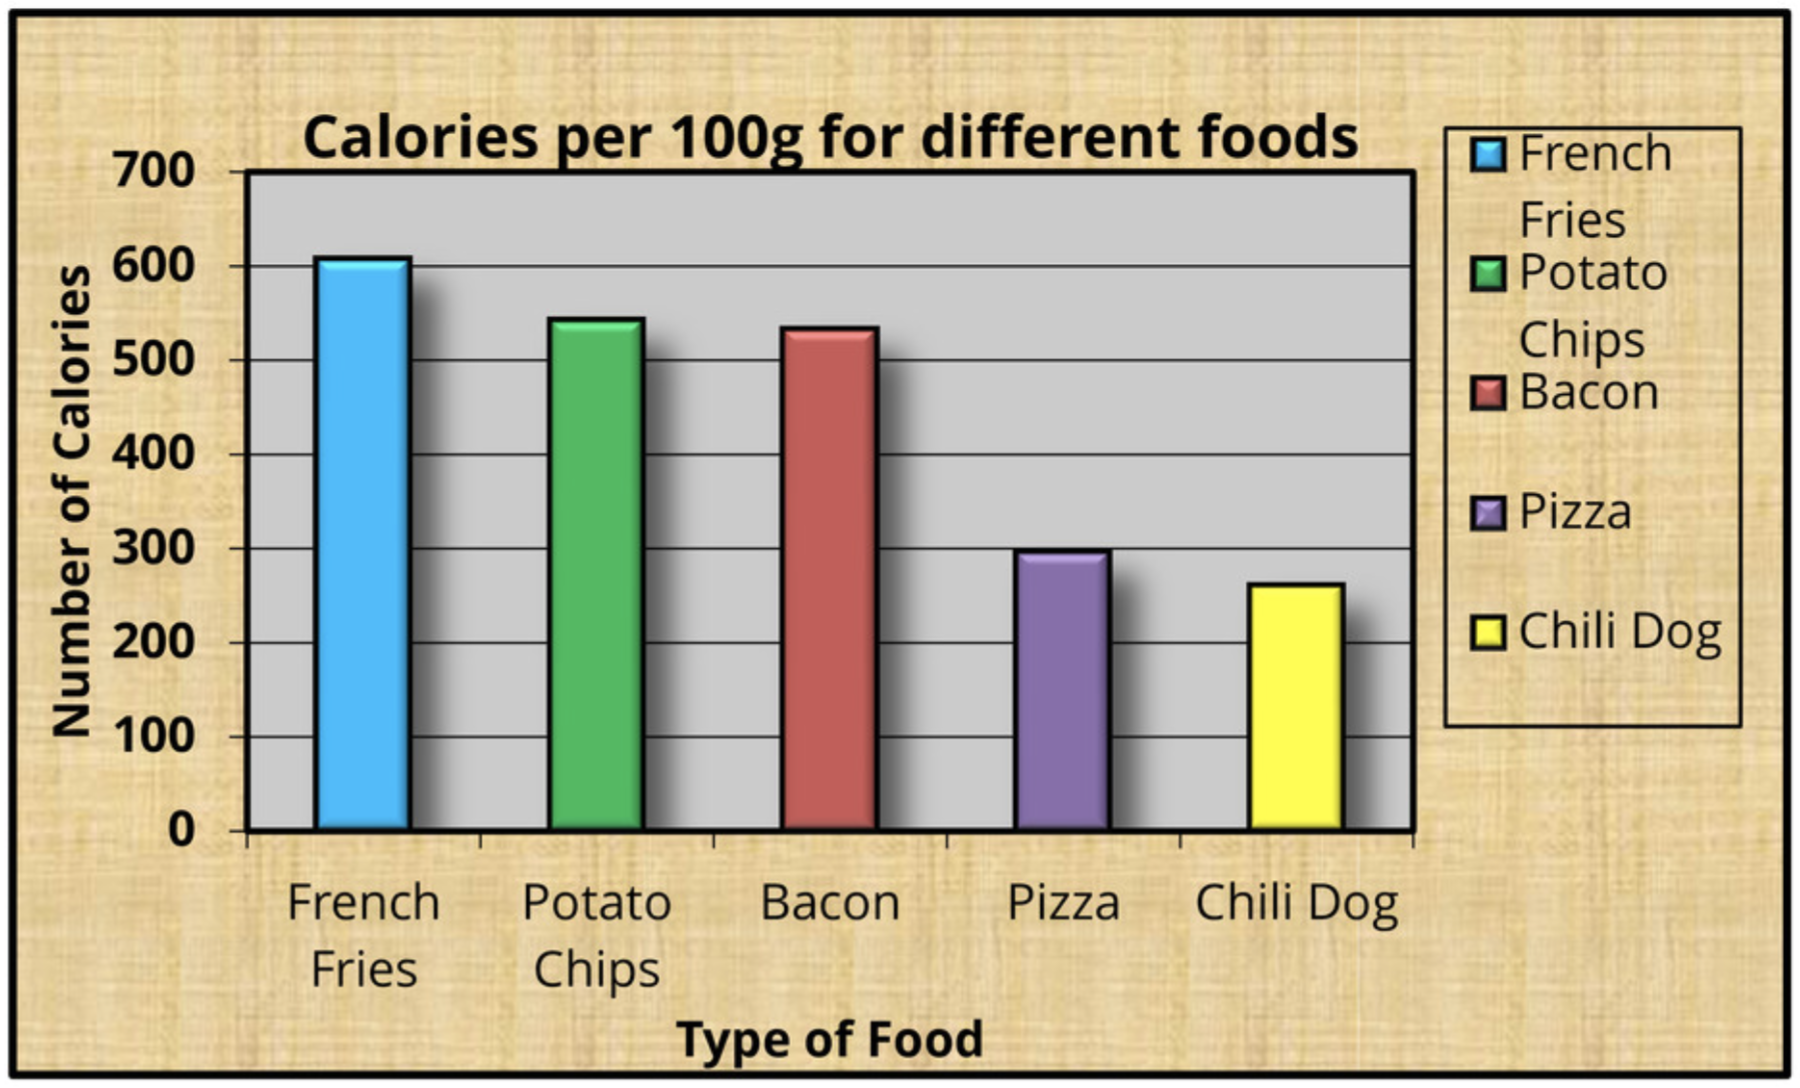
\includegraphics[width=0.48\textwidth]{barplot-before}%
\hspace{\fill}%
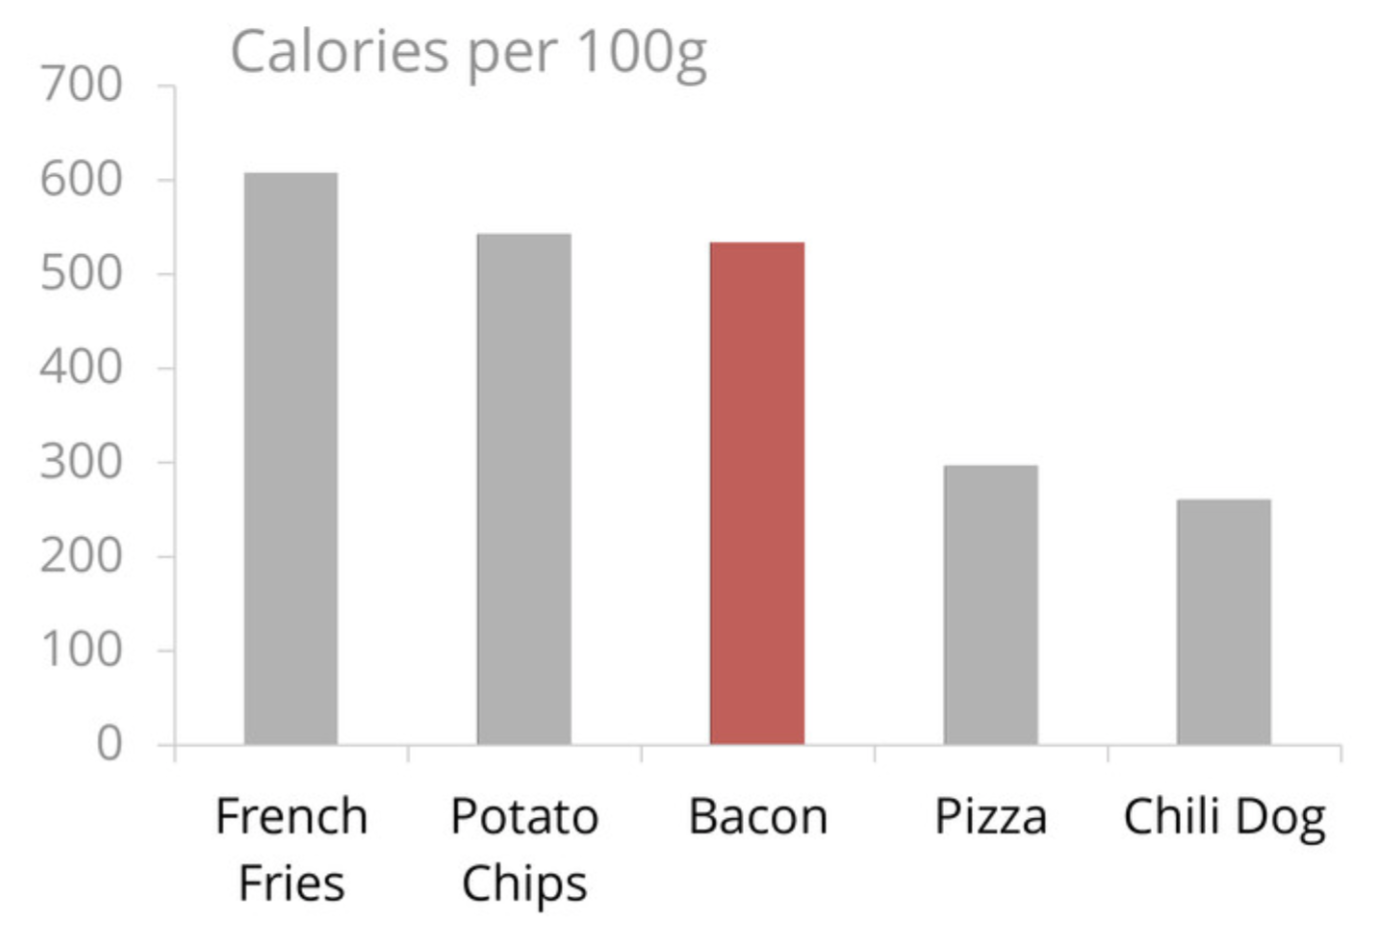
\includegraphics[width=0.48\textwidth]{barplot-after}
\sidecaption{\label{fig:barplot}%
   Removing unnecessary clutter.}[-2\baselineskip]
   % using optional last parameter: negative offset to correct vertical
   % position of caption (this caption is two lines high)
\end{figure}


Make sure that your figures work when \textbf{printed in monochrome}, i.\,e., you shouldn't rely on the colors too much. If you do use colors, use the same color palette in all figures, and ensure that readers with color blindness can differentiate all colors.

If you present plots of experimental results, use a tool that allows you to automatically \textbf{recreate plots}. To this end, you recommend to write scripts that create the plots based on raw data. Another benefit is that you will be able to change the design of all plots with little effort.%
\marginnote{\url{https://matplotlib.org}, \url{https://seaborn.pydata.org}, \url{https://ggplot2.tidyverse.org}, and \url{http://www.gnuplot.info}}
Common tools are Python's \textsc{matplotlib} (also consider using \textsc{seaborn}), R's \textsc{ggplot2}, and \textsc{gnuplot}. Make sure to export your plots as PDFs.

\subsubsection{Figure Layout Options}

Place your figures in the \file{figures} folder, which allows you to omit the directory name in the \verb|\includegraphics{filename}| command.
The following code produces Fig.~\ref{fig:Electron}:
\begin{latex}
\begin{figure}[t] % [t]: place at top of page (recommended)
\centering

\includegraphics[width=0.75\textwidth]{Electron}
\decoRule
\caption[An Electron]{An electron (artist's impression).}
\label{fig:Electron}
\end{figure}
\end{latex}

\begin{figure}[t] % [t]: place at top of page (recommended)
\centering

\includegraphics[width=0.75\textwidth]{Electron}
\decoRule
\caption[An Electron]{An electron (artist's impression).}
\label{fig:Electron}
\end{figure}

You can also use the custom command \code{image} for inserting a figure:

\begin{latex}
\image[h]{\textwidth}{Electron}{An electron (artist's impression).}{Electron}
\end{latex}

This command will produce the same result as the previously shown commands.
For further information on the usage of the custom commands you should take a look at the extensive documentation in \file{commands.tex} in the \emph{misc} folder.

Figures should appear on the page where they are referenced first or on one of the subsequent pages. The recommended \textbf{figure placement} is the top of the page (denoted by \code{[t]}). Don't worry about figures not appearing exactly where you write them in the source. Sometimes there is not enough room to fit a figure directly where it should go (in relation to the text) and so LaTeX puts it at the top of the next page.

Every figure needs a \textbf{descriptive caption and a label}. Figure captions must always appear below the included graphics file within the \code{figure} environment.

Every figure \textbf{must be referenced} in the text at least once, either in parentheses (cf. Fig.~\ref{fig:Electron}) or explicitly in the sentence: Figure~\ref{fig:Electron} shows an electron. Refer to figures using the abbreviation \code{Fig.} followed by a protected space (\verb|~|) and \verb|\ref|. Exception: write \code{Figure} if it is the first word of a sentence. Note \verb|Fig.| and \verb|Figure| are capitalized when they are used as part of a reference.

The \verb|\caption| command contains two parts,
the first part, inside the square brackets%
\sidenote{Theses at PSI usually do not have a List of Figures. You can, therefore, omit the part in square brackets.} 
is the title that will appear in the \emph{List of Figures}, and so should be short.
 The second part in the curly brackets should contain the longer and more descriptive caption text.

The \verb|\decoRule| command is optional and simply puts a horizontal line below the image. Such a line can be useful with figures that are not symmetrical or whose exterior is uneven at the bottom.

Resize your figures, ideally consistently, to an appropriate size, e.\,g., a fraction of \texttt{\textbackslash textwidth}. Check that the font size (after scaling) is consistent. This advice is especially important when you include figures with different aspect ratios.

LaTeX is capable of using images in PDF, JPG, and PNG format. Whenever possible, use \textbf{vectorized figures} (PDF). PDFs provide sharper results at smaller file sizes. If you \emph{have} to use pixel graphics, create them with a sufficiently high resolution (at least 300 dpi).


\paragraph{Wide Figures} You can also add wide figures that span the full width of a page. These should be placed at the top of the page. The following code creates the example figure (Fig.~\ref{fig:widefig}):
\begin{latex}
\begin{figure*}[t] % place at top
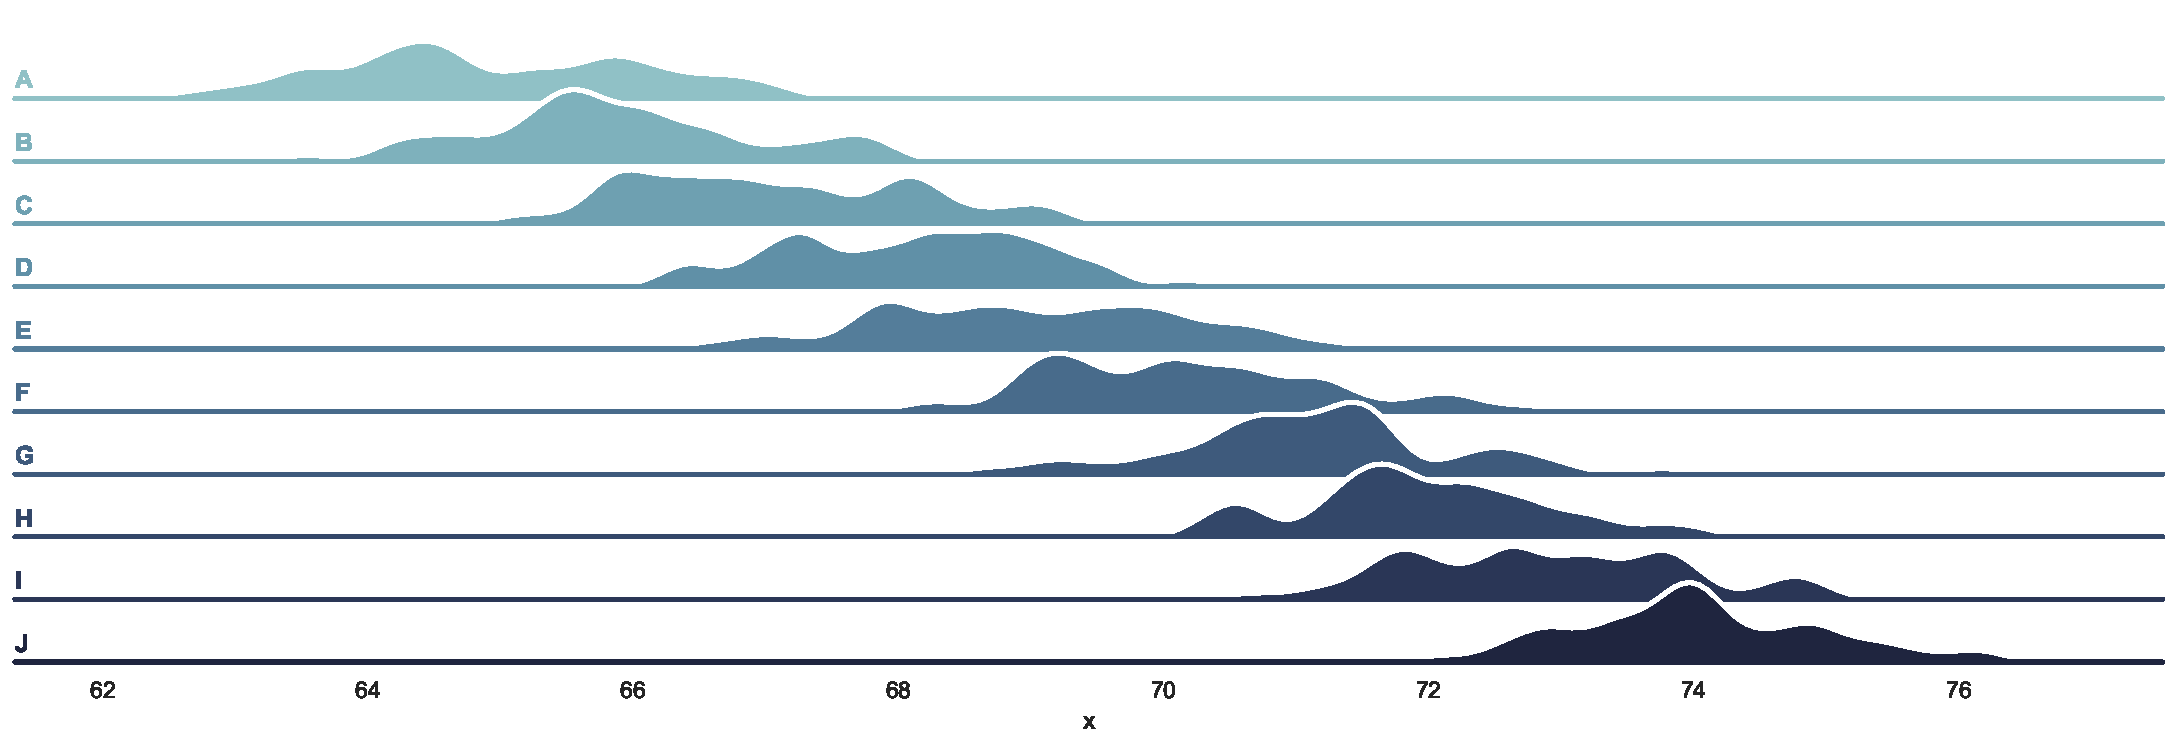
\includegraphics[width=\widefigurewidth]{plot.pdf}
\caption{\label{fig:widefig}
  This is a full-width figure. Lorem ipsum dolor sit amet, …
}
\end{figure*}
\end{latex}

\begin{figure*}[t]
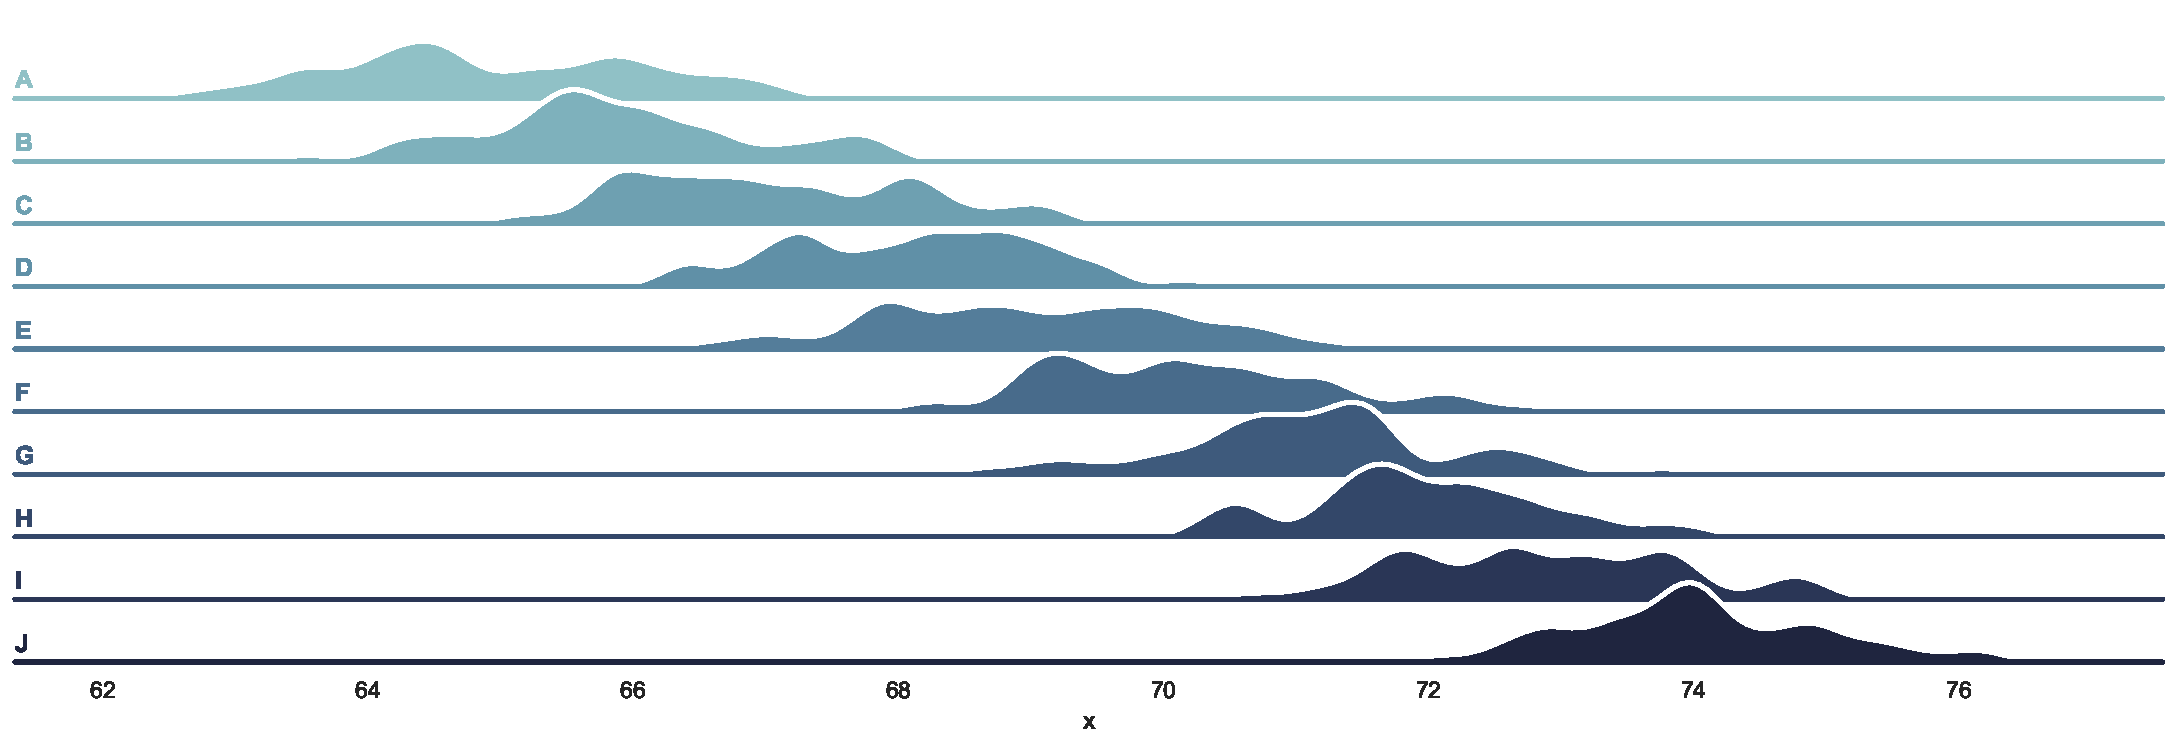
\includegraphics[width=\widefigurewidth]{plot.pdf}
\caption{\label{fig:widefig}This is a full-width figure. Lorem ipsum dolor sit amet, consectetur adipisicing elit, sed do eiusmod tempor incididunt ut labore et dolore magna aliqua. Ut enim ad minim veniam, quis nostrud exercitation ullamco laboris nisi ut aliquip ex ea commodo consequat.}
\end{figure*}

You can also use the custom command \code{wideimage} for inserting a figure:

\begin{latex}
\wideimage[h]{plot.pdf}{This is a full-width figure. Lorem ipsum dolor sit amet, …}{widefig}
\end{latex}

This command will produce the same result as the previously shown commands.
For further information on the usage of the custom commands you should take a look at the extensive documentation in \file{commands.tex} in the \emph{misc} folder.

Occasionally, LaTeX misplaces wide figures on the \textbf{horizontal axis}. For instance, figures may end up partly outside of the page instead of being properly aligned with the text block. Often, these problems happen only sporadically. Compiling \texttt{main.tex} again with a single invocation of \texttt{lualatex} will fix the layout.

\paragraph{Side-by-Side Figures} Sometimes it is desirable to show multiple figures next to each other. There are several approaches for that, e.\,g., using the \texttt{subfigure} package. In many cases, however, a comprehensive subfigure support is not needed. A lightweight approach as shown in Fig.~\ref{fig:barplot} may be sufficient. This result is achieved with the following code:
\begin{latex}
\begin{figure}[t]
\centering
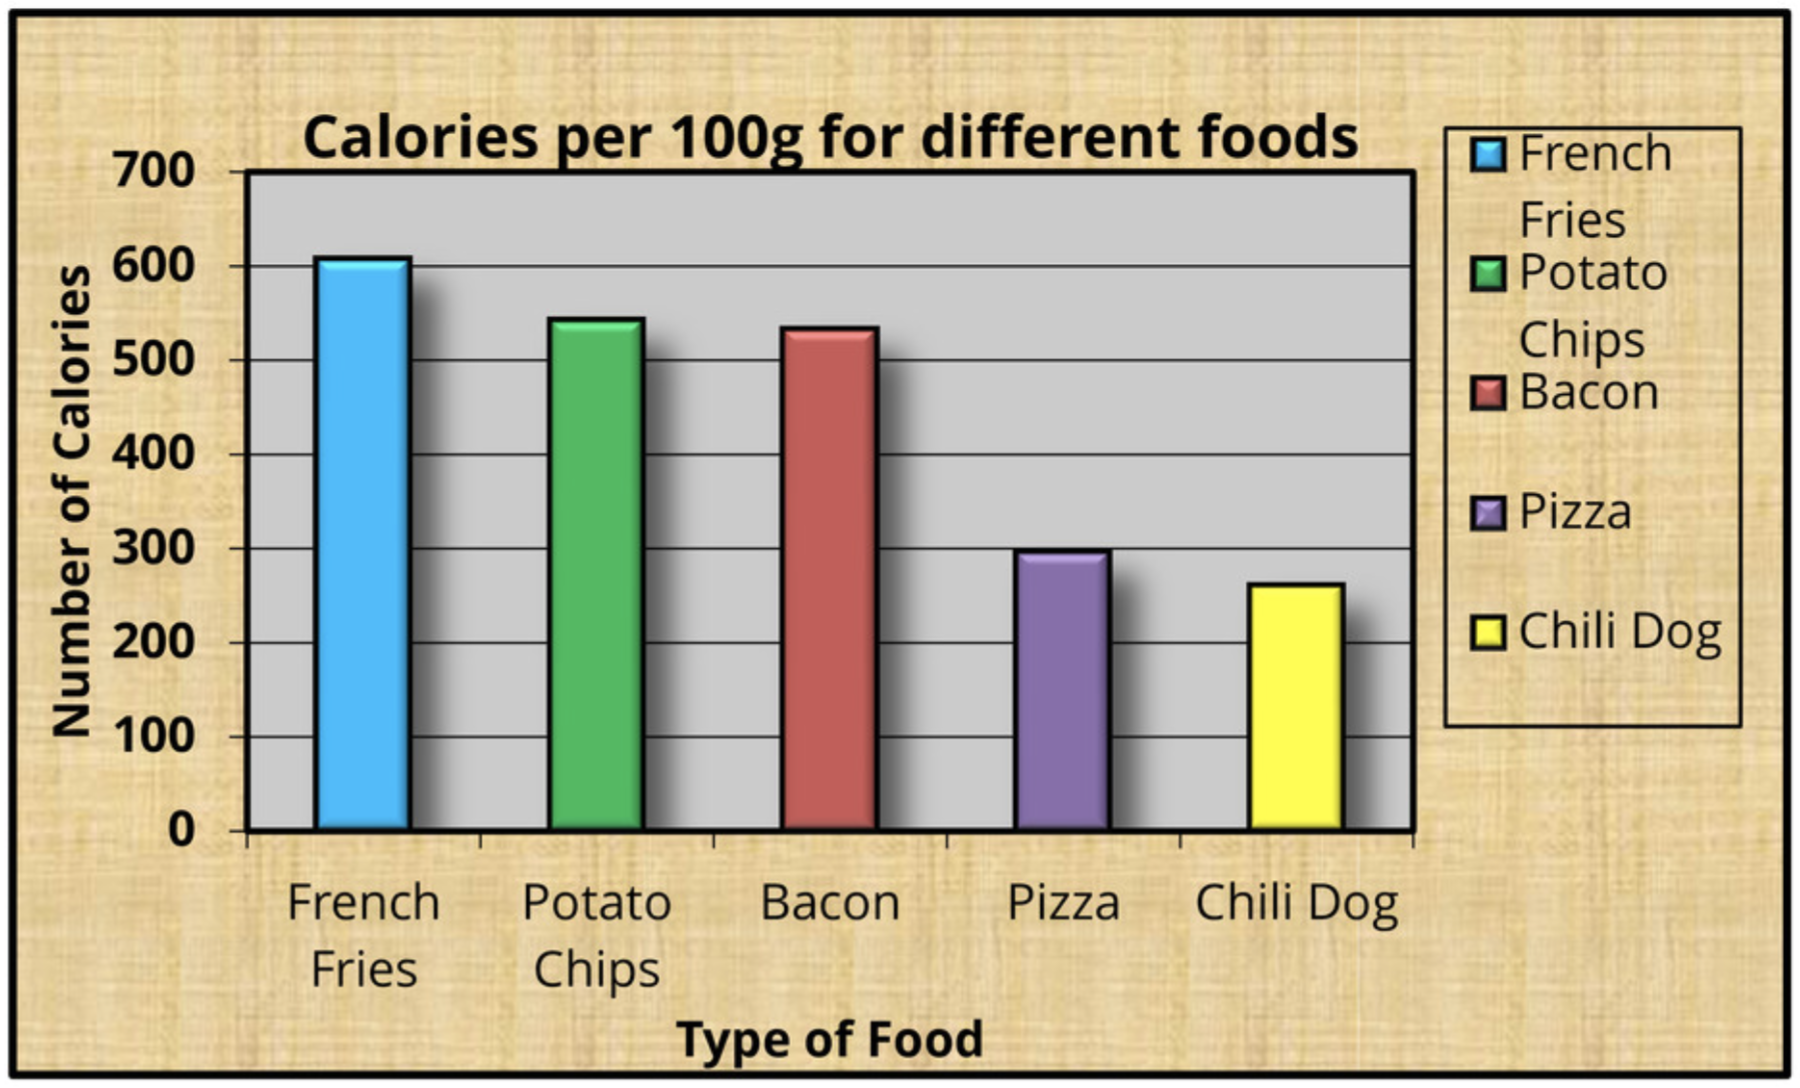
\includegraphics[width=0.48\textwidth]{barplot-before}%
\hspace{\fill}%
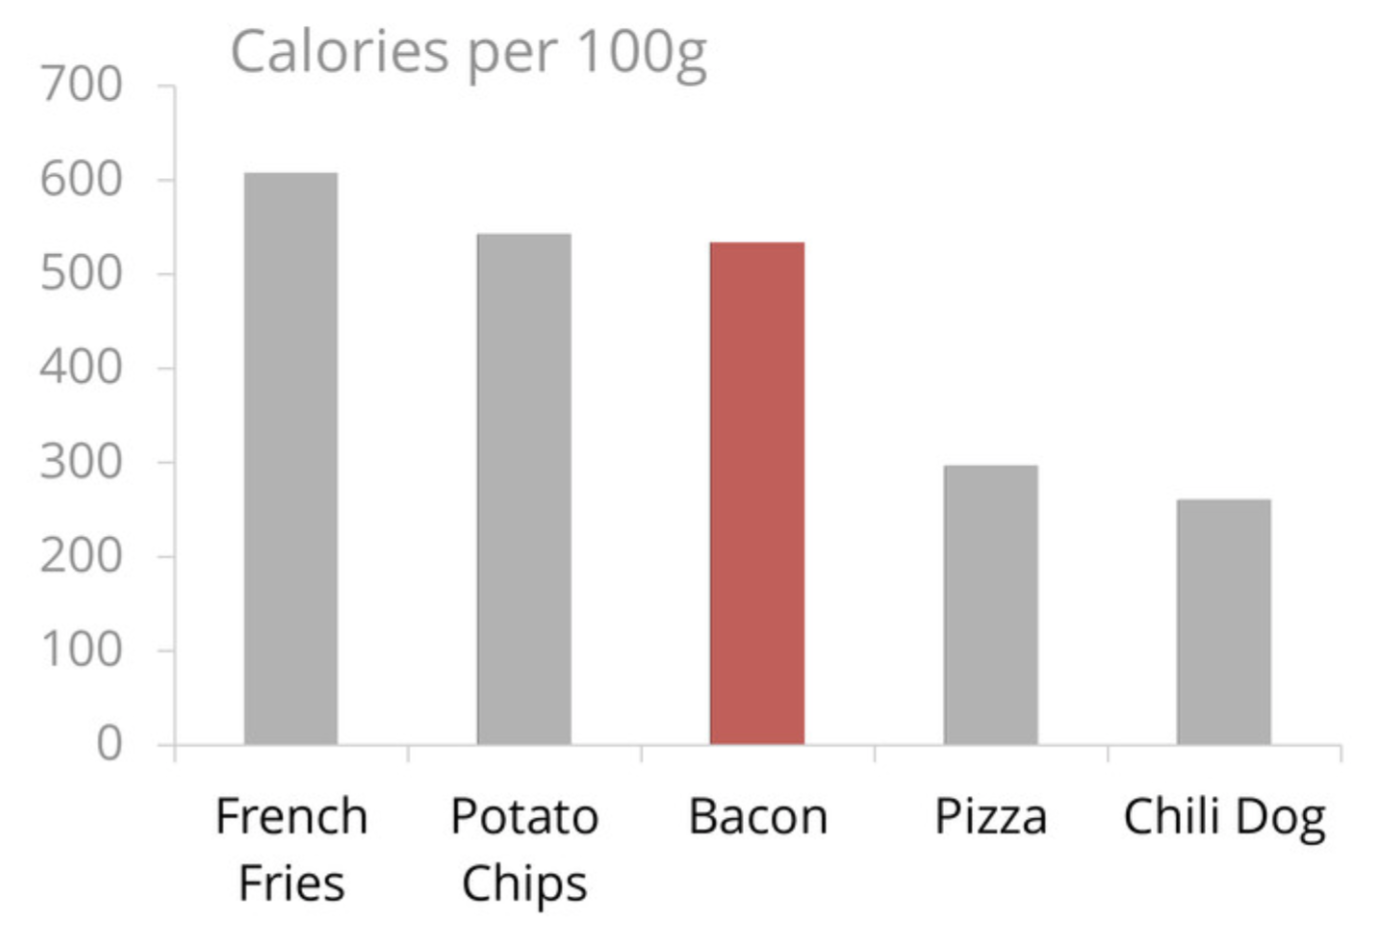
\includegraphics[width=0.48\textwidth]{barplot-after}
\sidecaption{\label{fig:barplot}%
   Removing unnecessary clutter.}[-2\baselineskip]
   % using optional last parameter: negative offset to correct vertical
   % position of caption (this caption is two lines high)
\end{figure}
\end{latex}

You can also use the custom command \code{twoimages} for inserting two figures next to each other:

\begin{latex}
\twoimages[h]{barplot-before}{barplot-after}{Removing unnecessary clutter.}{barplot}
\end{latex}

This command will produce the same result as the previously shown commands.
For further information on the usage of the custom commands you should take a look at the extensive documentation in \file{commands.tex} in the \emph{misc} folder.


Figure \ref{fig:barplot} uses a \textbf{side caption} (\code{sidecaption}). Whether you use side captions or not is up to you.
Just ensure to place all captions consistently, i.\,e., either in the margin or above or below floats for tables and figures, respectively. Note that \code{sidecaption} does not work with floating listings.

\begin{marginfigure}[-1\baselineskip] % move figure up by 1 line 

\includegraphics[width=\marginparwidth]{Electron}
\caption{\label{fig:marfig}This is a margin figure with a reasonably short caption.}
\end{marginfigure}

\paragraph{Margin Figures} Sometimes, it makes sense to place figures in the margin. Margin figures work best for figures that are simple and unobtrusive. They are a useful mechanism to include figures that illustrate concepts and for graphs that are meant to give an overall impression. Do not use margin figures for figures that convey essential results.
%
You can create margin figures like Fig.~\ref{fig:marfig} with the following code:
\begin{latex}
\begin{marginfigure}[-1\baselineskip] % move figure up by 1 line 

\includegraphics[width=\marginparwidth]{Electron}
\caption{\label{fig:marfig}This is a margin figure with a reasonably short caption.}
\end{marginfigure}
\end{latex}

You can also use the custom command \code{marginimage} for inserting a figure in the margin:

\begin{latex}
\marginimage[-1]{Electron}{This is a margin figure with a short caption.}{marfig}
\end{latex}

This command will produce the same result as the previously shown commands.
For further information on the usage of the custom commands you should take a look at the extensive documentation in \file{commands.tex} in the \emph{misc} folder.

\paragraph{Margin Tables} You can also place tables into the margin. Due to the limited space of the margin the content of a margin table should be carefully considered. Otherwise the table will clip into the main body or overflow over the page. In general, we recommend to create the table with the full width of the margin, otherwise the margin layout may become ragged. Moreover, we reduce the font size of margin tables to \emph{footnotesize} so that they do not attract too much attention.
%
You can create a full-width margin table like Table~\ref{tab:martab} with the following code:

% left-aligned table columns with automated line breaks 
\newcolumntype{L}{>{\RaggedRight\arraybackslash}X}
\begin{margintable}[1\baselineskip] % move figure down by 1 line
\caption{\label{tab:martab}This is a margin table with a short caption that spans two lines.}
\footnotesize
\begin{tabularx}{\textwidth}{@{}Lcc@{}}
\toprule
& \multicolumn{2}{c}{\tabhead{Observed results}} \\ \cmidrule(){2-3}
\tabhead{Group} & \tabhead{X} & \tabhead{Y} \\
\midrule
1 & 0.20 & 0.81\\
2 & 0.17 & 0.70\\
3 & 0.24 & 0.75\\
\bottomrule\\
\end{tabularx}
\end{margintable}

\begin{latex}
% left-aligned table columns with automated line breaks 
\newcolumntype{L}{>{\RaggedRight\arraybackslash}X}
\begin{margintable}[1\baselineskip] % move figure down by 1 line
\caption{\label{tab:martab}This is a margin table with a short caption that spans two lines.}
\footnotesize
\begin{tabularx}{\textwidth}{@{}Lcc@{}}
\toprule
& \multicolumn{2}{c}{\tabhead{Observed results}} \\ \cmidrule(){2-3}
\tabhead{Group} & \tabhead{X} & \tabhead{Y} \\
\midrule
1 & 0.20 & 0.81\\
2 & 0.17 & 0.70\\
3 & 0.24 & 0.75\\
\bottomrule\\
\end{tabularx}
\end{margintable}
\end{latex}

\subsection{Listings}

If you are new to LaTeX, we recommend to use the \emph{listings} package for code listings.%
\sidenote{If you have Python, you can consider the more modern package \code{minted}, which uses \code{pygments} for syntax highlighting.}
With the template's default monospace font, lines can have up to 70 characters. Longer lines are automatically wrapped. An arrow at the end of the line indicates the line wrapping. Format your listing in such a way that the number of wrapped lines is low to improve readability.

You can create floating listings, which behave very much like floating figures and tables, i.\,e., they have a caption and can be referenced (cf. Listing~\ref{lst:listing} for an example).\sidenote{As of now, the template does not offer wide listings that span the text and the margin.} Sometimes, however, the properties of floating listings are undesirable. For short code fragments, it often makes more sense to use a non-floating listing.

Listing~\ref{lst:listing} has been generated with the following code:
\begin{latex}
\begin{lstlisting}[language=Python,float=t,
  caption={This is an example of syntax highlighting of
  Python code with a relatively long caption},label={lst:listing}]
import numpy as np

test = "This is a test string"
 
def incmatrix(genl1,genl2):
    ...
    return M
\end{lstlisting}
\end{latex}

\begin{lstlisting}[language=Python,float=t,
  caption={This is an example of syntax highlighting of
  Python code with a relatively long caption},label={lst:listing}]
import numpy as np

test = "This is a test string"
 
def incmatrix(genl1,genl2):
    m = len(genl1)
    n = len(genl2)
    M = None # to become the incidence matrix
    VT = np.zeros((n*m,1), int)  # dummy variable
 
    # compute the bitwise xor matrix
    M1 = bitxormatrix(genl1)
    M2 = np.triu(bitxormatrix(genl2),1) 
 
    for i in range(m-1):
        for j in range(i+1, m):
            [r,c] = np.where(M2 == M1[i,j])
            for k in range(len(r)):
                VT[(i)*n + r[k]] = 1;
                VT[(i)*n + c[k]] = 1;
                VT[(j)*n + r[k]] = 1;
                VT[(j)*n + c[k]] = 1;
 
                if M is None:
                    M = np.copy(VT)
                else:
                    M = np.concatenate((M, VT), 1)
 
                VT = np.zeros((n*m,1), int)
 
    return M
\end{lstlisting}


\section{Mathematics}

The \enquote{Not So Short Introduction to LaTeX}\sidenote{\url{http://www.ctan.org/tex-archive/info/lshort/english/lshort.pdf}} should tell you everything you need to know for most cases of typesetting mathematics. If you need more information, a much more thorough mathematical guide is available from the AMS.\sidenote{``A Short Math Guide to LaTeX,'' available at \url{ftp://ftp.ams.org/pub/tex/doc/amsmath/short-math-guide.pdf}}

There are many different LaTeX symbols to remember, luckily you can find the most common symbols in ``The Comprehensive \LaTeX~Symbol List'' (\url{http://ctan.org/pkg/comprehensive}).

You can write a numbered equation like this:
\begin{latex}
\begin{equation}
E = mc^{2}
\label{eqn:Einstein}
\end{equation}
\end{latex}

This will produce Einstein's famous energy-matter equivalence equation:
\begin{equation}
E = mc^{2}
\label{eqn:Einstein}
\end{equation}

LaTeX automatically gives all equations you write equation numbers. If you don't want a particular equation numbered, use the unnumbered form:
% use of verbatim here because we do not need syntax highlighting and want to avoid lstlsting style for a one-line listing
\begin{verbatim}
\[ a^{2}=4 \]
\end{verbatim}

You can also have equations in the middle of a paragraph, e.\,g., \( x = \sum_{i=1}^{10} \cdot \hat{a} \cdot \frac{\alpha}{\psi} \cdot i^{2^3} \), with this syntax: 
% use of verbatim here because we do not need syntax highlighting and want to avoid lstlsting style for a one-line listing
\begin{latex}
e.\,g., \( x = \sum_{i=1}^{10} \hat{a} \cdot \frac{\alpha}{\psi} \cdot i^{2^3} \), with this syntax:
\end{latex}

%----------------------------------------------------------------------------------------

\section{Structuring Your Thesis}

You should break your thesis up into chapters and sections. LaTeX automatically builds a Table of Contents by looking at all the \verb|\chapter{}|, \verb|\section{}|  and \verb|\subsection{}| commands you write in the source. You may even think about using \emph{sub}subsections (\verb|\subsubsection{}|). All of these will be hierarchically numbered.

Use \textbf{(sub-)subsections} only if you use them consistently in all or at least multiple chapters. Otherwise, you should opt for a \verb|paragraph{}|, which structures pieces of content with bold non-numbered inline headings (examples throughout this guide).

\textbf{Avoid dangling elements} in the hierarchy: If you have a Section~1.1, you should also have (at least) Section~1.2. This rule applies to all levels of the hierarchy.

The Table of Contents is configured to only list \emph{chapters} and \emph{sections}. We do not recommend to include \emph{(sub-)subsections} as this results in a very long Table of Contents, which may become difficult to read. If you do want to change the depth of the Table of Contents, you can change the value \verb|\etocsettocdepth| in \file{setup.tex}.

Use \textbf{title case} in \emph{chapter}, \emph{section}, \emph{(sub)subsection}, and \emph{paragraph} environments. Consider, for instance, \url{https://capitalizemytitle.com} for common title case capitalization rules.

Within a section, you should \textbf{walk the reader through your text}:
\begin{quote}
In the following, we describe the three primitives of concept X. First, X uses the Y algorithm. …

The second concept is Z …
\end{quote}

\section{Typography}

Use emphasis sparingly. This advice is especially true for \textbf{bold print} (\verb|\textbf{bold print}|).%
\sidenote{To allow for fast skimming, we use bold print liberally throughout this guide (which would not be appropriate in a thesis).}
Resist the urge to use it in the main text; use \emph{italics} (\verb|\emph{italics}|) instead.

Note, however, that \textbf{too frequent use of italics} can also be annoying.
We recommend using it to emphasize ordinary words that are used as special terms – and only at its first occurrence. Also, you should emphasize words that you would stress when reading aloud, indicating that they are especially relevant for the meaning. Do not mix italics and quotes for emphasis, because this confuses the reader.\sidenote{More on the topic ``Italics or Scare Quotes?'' is available at \url{https://sblhs2.com/2016/09/15/italics-scare-quotes/}.}


Generally, we recommend \textbf{avoiding scare quotes}.%
\sidenote{Reasons given in ``Quotes When Nothing Is Being Quoted'', which is available at \url{https://style.mla.org/quotes-when-nothing-is-being-quoted/}.}
Some authors use scare quotes to signal that they are using a word in a non-standard, ironic, or otherwise special sense (cf. Chicago Manual of Style). Scare quotes convey an informal tone. Moreover, they cause ambiguity, as the reader cannot be sure about the intention of the author.

You should split your content into \textbf{proper paragraphs} by adding empty lines between adjacent blocks of text in the source file. Using a mixture of paragraphs and line breaks, which you could create with \verb|\\| at the end of a line, is strongly discouraged because this practice creates a noisy layout.

Use \textbf{thin spaces} (\verb|\,|) in the appropriate places. For instance, write \verb|i.\,e.,| to obtain ``i.\,e.,'' (pronunciation: ``that is''). The same applies to ``e.\,g.,'' (pronunciation: ``for example''). These two abbreviations are normally followed by a comma in American English.

\textbf{Dashes} can be used instead of colons or pairs of commas to mark off a nested clause. Use an \emph{en dash} for that purpose -- like in this example. If you cannot type an \emph{en dash} on your keyboard, you can write two regular hyphens next to each other. LaTeX will substitute them with an \emph{en dash}. While we have no strict preference, we recommend using \emph{en dashes} instead of the longer \emph{em dashes}.

Use en dashes also for ranges, e.\,g., when you write something like 5--10\,\% (note the thin space before the \% symbol).

Use a proper \textbf{minus symbol} (e.\,g., by using math mode like this \(-1.337\)). Also, use a sensible number of digits after the decimal point.\sidenote{Have you noticed that the main text uses \emph{old-style figures} for numbers, while math mode uses \emph{lining figures}? Do not  print numbers with differing figure styles close to each other (as we are doing in this section).}

Use proper \textbf{directional quotation marks} like ``these.'' Directional quotation marks are created  \verb|``like this''|, by using \verb|\enquote{text}|, or by copy-and-pasting the respective Unicode characters. Note that in contrast to conventions in the German language, the closing quotation mark is placed \emph{after} any subsequent punctuation, e.\,g., ``like this,'' and ``like that.''

\paragraph{Further Reading}

If you speak German, consider reading \textsc{typokurz} (\url{https://zvisionwelt.wordpress.com/downloads/}), a short introduction to typographic issues. You can also browse Matthew Butterick's website \url{https://practicaltypography.com}.

\section{Language and Style}

Language issues distract readers from the content and make it difficult to assess its merits. You should, therefore, pay close attention to language and style.

\subsection{Spelling, Hyphenation, and Grammar}

Ensure correct spelling throughout your text. Check your writing with a spell checker. There are special spellcheckers for LaTeX, but copy-and-pasting the text into Word may also be an option.

Ensure proper hyphenation throughout your text. You will have to intervene, for instance, when words extend into the margin of the page (creating so-called overfull hboxes). You can override LaTeX's hyphenation rules by inserting \verb|\-| into a word. This special character indicates a conditional hyphenation point.

Often, it makes sense to define custom hyphenation rules globally. To this end, define your custom hyphenation definitions with\verb|\hyphenation{FORTRAN Hy-phen-a-tion}| and insert them after the \verb|\begin{document}| clause.\todo[noline]{Oh no, an overful hbox!}\ 
The example definition prevents any hyphenation of the word FORTRAN and defines three hyphenation points for the word Hyphenation.

Also, check your text for common grammar issues (cf. Sect.~\ref{sec:style}).

\subsection{Style}
\label{sec:style}

This section contains selected pieces of advice on particular aspects and typical errors. For a more comprehensive treatment, we refer the reader to the paragraph \nameref{par:commonbugs} at the end of this section.

The main goal of a thesis is to convey information without ambiguity. Write concisely and use a simple language. Avoid complex sentence structures, unnecessary words, and unnecessarily complicated words. A thesis is not the place to show off your mastery of grammar and vocabulary. There are various (mostly web-based and commercial) tools%
\sidenote{\url{http://hemingwayapp.com}, \url{https://grammarly.com}, \url{https://languagetool.org}, and the command-line tool (\url{https://github.com/devd/Academic-Writing-Check}).}
that can help you identify common issues in your text.


\subsubsection{The Science of Scientific Writing}

Even if a text uses a simple language, it may be difficult to read, because it does not convey the writer's train of thoughts coherently. In short, your goal is to connect every sentence explicitly to its predecessor – which is, of course, easier said than done.

A good resource to develop this skill is the article \emph{The Science of Scientific Writing} by George D. Gopen and Judith A. Swan.\sidenote{The article can be obtained from \url{https://cseweb.ucsd.edu/~swanson/papers/science-of-writing.pdf} and \url{https://www.americanscientist.org/blog/the-long-view/the-science-of-scientific-writing}.} 
The advice from this article is also part of the three lessons on scientific writing offered by Duke University.\sidenote{Homepage of the lessons: \url{https://cgi.duke.edu/web/sciwriting/}, PDF slides: \url{https://cgi.duke.edu/web/sciwriting/resources/201108_DukeScientificWritingWorkshop.pdf} (these URLs could not be archived).}

The remainder of this section contains selected excerpts from \emph{The Science of Scientific Writing}. Consider reading the original article for a more extended treatment, including worked examples.

\paragraph{Subject-Verb Separation (Excerpts)}

  Readers expect a grammatical subject to be followed immediately by the verb. Anything of length that intervenes between subject and verb is read as an interruption, and therefore as something of lesser importance.
The reader’s expectation stems from a pressing need for syntactic resolution, fulfilled only by the arrival of the verb. Without the verb, we do not know what the subject is doing, or what the sentence is all about.

As a result, the reader focuses attention on the arrival of the verb and resists recognizing anything in the interrupting material as being of primary importance.
The longer the interruption lasts, the more likely it becomes that the “interruptive” material actually contains important information; but its structural location will continue to brand it as merely interruptive.
Unfortunately, the reader will not discover its true value until too late – until the sentence has ended without having produced anything of much value outside of the subject-verb interruption.

\paragraph{The Stress Position (Excerpts)}

It is a linguistic commonplace that readers naturally emphasize the material that arrives at the end of a sentence. We refer to that location as a “stress position.”
Beginning with the exciting material and ending with a lack of luster often leaves us disappointed and destroys our sense of momentum.

The stress position can change in size from sentence to sentence. Sometimes it consists of a single word; sometimes it extends to several lines. The definitive factor is this: The stress position coincides with the moment of syntactic closure. A reader has reached the beginning of the stress position when she knows there is nothing left in the clause or sentence but the material presently being read.

To summarize the principles connected with the stress position, we have the proverbial wisdom, “Save the best for last.”

\paragraph{The Topic Position (Excerpts)}

To summarize the principles connected with the other end of the sentence, which we will call the topic position, we have its proverbial contradiction, “First things first.”
In the stress position the reader needs and expects closure and fulfillment; in the topic position the reader needs and expects perspective and context.

The information that begins a sentence establishes for the reader a perspective for viewing the sentence as a unit: Readers expect a unit of discourse to be a story about whoever shows up first. “Bees disperse pollen” and “Pollen is dispersed by bees” are two different but equally respectable sentences about the same facts. The first tells us something about bees; the second tells us something about pollen. In fact, “Pollen is dispersed by bees” is the superior sentence if it appears in a paragraph that intends to tell us a continuing story about pollen. Pollen’s story at that moment is a passive one.

Readers also expect the material occupying the topic position to provide them with linkage (looking backward) and context (looking forward).

\subsubsection{Selected Syntactical Conventions}

Avoid using \textbf{informal contractions} such as \emph{can't}, \emph{don't}, and \emph{it's}. Replace them with \emph{cannot}, \emph{do not}, and \emph{it is}.

We recommend using the \textbf{serial comma} in all lists to avoid ambiguity. The serial comma is also known as the \emph{Oxford comma}: Insert  it right before the word \emph{and} that leads the last item of a list. The following example%
\sidenote{Source: \url{https://nhigham.com/2016/02/16/the-serial-or-oxford-comma/}}
illustrates the benefit of using a serial comma:
\begin{quote}
  Three important techniques in the design of algorithms are bisection, divide and conquer, and recursion.
\end{quote}

Use \textbf{bullet lists} correctly. ``Lists are common in all forms of writing. The list items can be included within the text or put on separate lines. Separate lines are used in order to draw attention to the items, to ease reading when the items are long or numerous, or to facilitate cross-reference to specific items.''\sidenote{Source of cited text: \url{https://nhigham.com/2015/12/17/punctuating-lists/}.} The environments \code{itemize} and \code{enumerate} produce lists on separate lines. It is considered good style to use punctuation in such a way that the lists form full sentences if their items were \emph{not} split into separate lines. One way to achieve this goal is to only put full sentences into the list. If list items, however, are sentence fragments, additional punctuation is necessary (example taken from source mentioned in footnote):

\begin{quote}
  We used three different algorithms in the experiments. The table reports the performance of
\begin{itemize}
\item Algorithm 3.1 (based on a Taylor series),
\item Algorithm 3.2 (with parameter \(k = 1\)), and
\item Algorithm 3.3 (with tolerance \(10^{-8}\)).
\end{itemize}
\end{quote}

\paragraph{Common Bugs in Writing}
\label{par:commonbugs}
Read the comprehensive list of common bugs in writing by Henning Schulzrinne, which is available at \url{http://www.cs.columbia.edu/~hgs/etc/writing-bugs.html}.

\section{Concluding Remarks}

Scientific work and writing are skills that you can practice. Seminar papers serve that purpose during the studies. The final thesis shows which methodical and technical skills you have acquired. In addition to proper time management, discipline, and willingness to research literature, communication with one's supervisor is the key to success.

\paragraph{Further Reading}

This guide is not meant to cover all topics of scientific writing in detail. Consider the very comprehensive document \emph{Scientific Writing for Computer Science Students} by Wilhelmiina Hämäläinen.%
\sidenote{Available at \url{http://www.cs.joensuu.fi/pages/whamalai/sciwri/sciwri.pdf}.}
Hämäläinen has collected a substantial amount of advice with a particular focus on English grammar and the peculiarities of computer science.

There is also an abundant number of books on scientific writing. We can recommend the following:
\begin{itemize}
\item M. Alley. The Craft of Scientific Writing; and
\item W. Strunk and E.B. White. The Elements of Style.
\end{itemize}

Finally, if you seek inspiration, we recommend to read these reports by well-known scientists:
\begin{itemize}
\item Randy Pausch: Time Management (\url{http://www.youtube.com/watch?v=oTugjssqOT0}),
\item Richard Hamming: You and Your Research (\url{http://www.cs.virginia.edu/~robins/YouAndYourResearch.html}), and
\item Nick Feamster: Writing Tips for Academics (\url{http://greatresearch.org/2013/10/11/storytelling-101-writing-tips-for-academics/}).
\end{itemize}

The remaining parts of this guide contain less-often needed technical details and historical information about the template as well as a loose collection of assorted advice.
%\input{chapters/chapter3.tex}
%\input{chapters/chapter4.tex}
%\input{chapters/chapter5.tex}


%----------------------------------------------------------------------------------------
%	THESIS CONTENT - APPENDICES
%----------------------------------------------------------------------------------------

% By using input instead of include for the chapters we are able to move the following line here
% Therefore the addition before the last chapter is not necessary anymore.

% Call the following chapters "Appendix" inside the table of contents
\addtocontents{toc}{\string\def\string\chaptername{Appendix}}

\appendix % Cue to tell LaTeX that the following "chapters" are Appendices

% Ensure proper section numbering in appendix, e.g., A.1, A.2, B.1, …
\renewcommand{\thesection}{\thechapter.\arabic{section}}
\renewcommand{\thesubsection}{\thesection.\arabic{subsection}}
\renewcommand{\thesubsubsection}{\thesubsection.\arabic{subsubsection}}

%%% CHANGES NEEDED HERE
%
% Include the appendices of the thesis as separate files from the Appendices folder
% Uncomment the lines as you write the Appendices

% Appendix A
 
\chapter{Further Recommendations}

This appendix contains further recommendations, which our students found useful in the past.

\section{Introduction, Related Work, and Conclusion}

\subsection{Introduction Chapter}

Don’t be boring! Pull in the reader with a peculiar observation or a surprising result of your thesis.

Approaches to structure your introduction:
\begin{itemize}
\item Start with the general, close with the specific.
\item Start with what is already well-known, move on to what has only recently become known.
\item State the objective of the thesis, then describe your approach.
\end{itemize}

End the introduction with a paragraph \emph{Outline of the Thesis} that describes its structure in prose.

\subsection{Related Work Chapter}

Think about a story and which message you want to convey. Some common themes are:
\begin{itemize}
\item “It used to be a difficult problem, but we know how to solve it.”
\item “While a lot of proposals exist, none has gained traction in reality. X found that one of the primary reasons for that situation is …”
\item “The field is a cat-and-mouse game between refined attacks and defenses. A common theme is … and overlooked areas are …”
\item “While most of the current literature focuses on X, it would make sense to apply techniques from field Y to the problem. One could then refine the problem as …”
\end{itemize}

\subsection{Conclusion Chapter}

A basic recipe for a conclusion chapter:
\begin{itemize}
\item a summary,
\item a critical assessment of what you have achieved,
\item pointers to related other topics,
\item a statement of the impact of the results, and
\item pointers to future work.
\end{itemize}

\section{Thesis Length}

Typical theses range from 25 to 100 pages. Do not worry too much about the page count. Write everything that is necessary to assess and reproduce your work, but no more. Less is more!

Check the individual parts for an appropriate length: Do not write five pages in the introduction if the main part has only 15 pages.


\section{Practices to Avoid}

\begin{itemize}
\item Colloquial style: “Computation power has skyrocketed in the last few years.”
\item Widespread knowledge: “The Internet is becoming more and more important.”
\item Superlatives: “One of the most beautiful concepts”, “great possibilities.”
\item Be careful with strong claims: “the only possibility”, “the best solution”, “impossible.”
\end{itemize}
% Appendix B
 
\chapter{Designing Figures and Tables}
\label{cha:designingfigtab}
\label{appendixb}

In Section~\ref{sec:tablesfigureslistings}, we have shown how you can integrate tables, figures, and listings into your thesis. In this appendix, we give recommendations on a higher level. In the following sections, we focus on \emph{designing} compelling figures and tables, i.\,e., how you can present material effectively. For figures, we will cover both graphs as well as diagrams.

We\marginnote{While this guide is published under a Creative Commons license (cf. Sect.~\ref{sec:license}), this license does not apply to the reproduced figures. Elsevier and/or the authors hold the copyright for the reproduced figures.}
have compiled most of the content in this appendix from the following two books (permission to reproduce the respective figures has been obtained from Elsevier):
\begin{itemize}
  \item the book \emph{Designing Science Presentations: A Visual Guide to Figures, Papers, Slides, Posters, and More} by Matt Carter, © 2012 \cite{Carter12} and
  \item the book \emph{Information Visualization: Perception for Design} by Colin Ware, © 2012 \cite{Ware12}.
\end{itemize}

Another useful resource is the book \emph{Universal Principles of Design: 125 Ways to Enhance Usability, Influence Perception, Increase Appeal, Make Better Design Decisions, and Teach Through Design} \cite{Lidwell10}.
  
\section{Fundamental Concepts}

We start by revisiting the fundamentals of visual perception as well as information organization. The following section will apply the concepts shown in this section.

When you design figures, you should be aware of the Gestalt laws and the HSB color model, which will be described in the following two sections. After that, we will revisit the basics of information organization, which apply to figures and tables alike.

\subsection{Gestalt Laws}

The Gestalt laws have been known since the early 1900s. They describe how we perceive patterns. In the following, we will discuss the following Gestalt laws: proximity, similarity, connectedness, continuity, symmetry, closure, and relative size.

\begin{marginfigure}
\centering
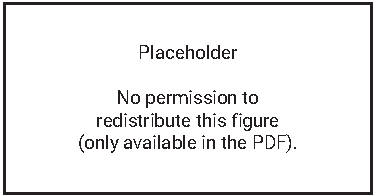
\includegraphics[width=1\textwidth]{gestalt-proximity}
\caption{\label{fig:proxi} Spacing makes us perceive rows or columns (reproduced from \cite{Ware12} with permission).}%[-1\baselineskip]
\end{marginfigure}


The first law, \textbf{proximity}, refers to the spatial relationships between groups of objects. Objects that are closer together form a group. We are very sensitive to spatial relationships. Even small changes in spacing can change our interpretation of a scene (cf. Fig.~\ref{fig:proxi}). Therefore, you should ``place symbols and glyphs representing related information close together.'' 
\cite{Ware12}. The proximity law is the reason why adding additional vertical space between (groups of) rows helps us with reading a table.

\begin{marginfigure}[-2\baselineskip]
\centering
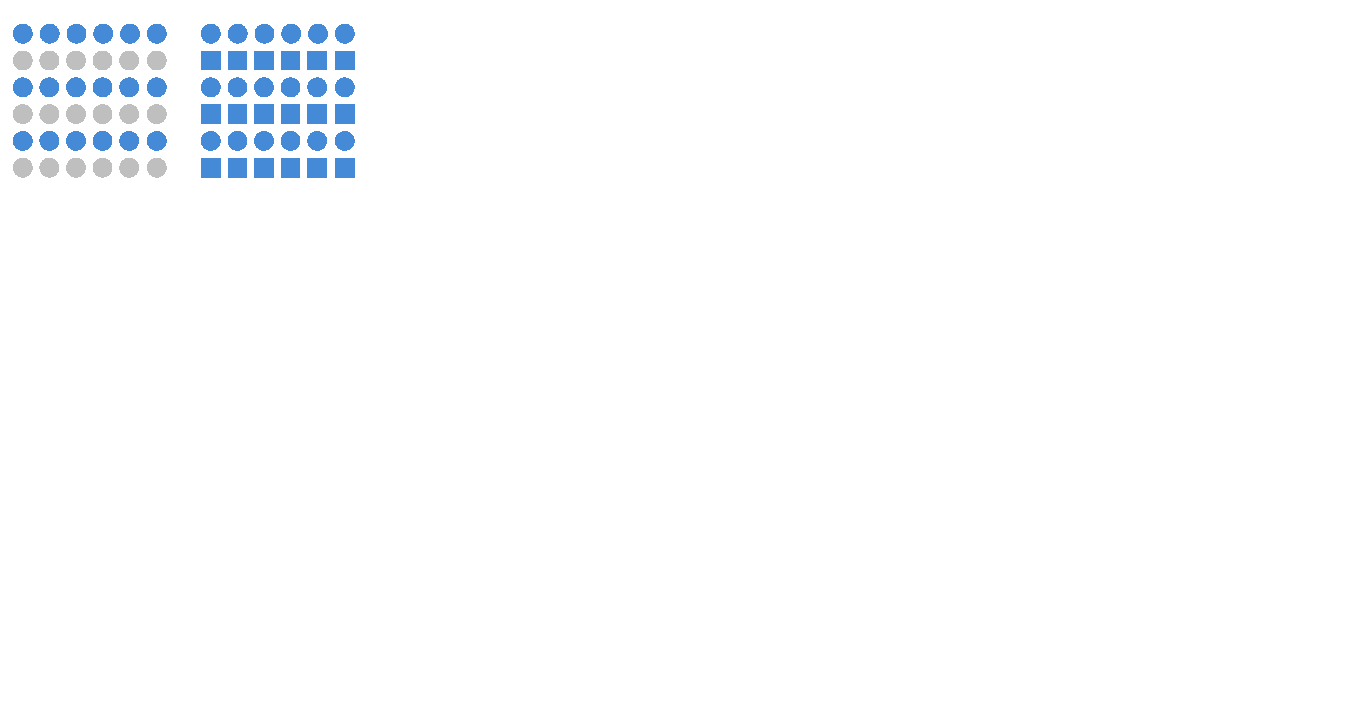
\includegraphics[width=1\textwidth]{gestalt-similarity}
\caption{\label{fig:simi} We perceive similar elements as a group (reproduced from \cite{Ware12} with permission).}
\end{marginfigure}

\textbf{Similarity} is the second Gestalt law. Visual similarities such as color or shape allow us to identify groups of objects with ease (cf. Fig.~\ref{fig:simi}). Large tables, for instance, can benefit from alternated shading of rows. A downside of shading is the additional visual clutter. We prefer to add extra space every three to five rows to keep tables readable. The similarity law is also essential in diagrams that use different shapes or styles. Visual differences help the reader group similar elements.


\textbf{Connectedness} is a powerful principle that is stronger than proximity, shape, and style (cf. Fig.~\ref{fig:connectedness}). Consider connecting related objects with lines.
\begin{marginfigure}[-2\baselineskip]
\centering
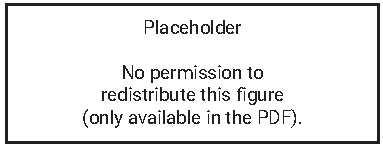
\includegraphics[width=1\textwidth]{gestalt-connectedness}
\caption{\label{fig:connectedness} Connections are more powerful than similarity (reproduced from \cite{Ware12} with permission).}
\end{marginfigure}

The next principle, \textbf{continuity}, ``states that we are more likely to construct visual entities out of visual elements that are smooth and continuous, rather than ones that contain abrupt changes in direction'' \cite{Ware12}. It is, therefore, not surprising that node-link diagrams with smooth lines are easier to read than those with straight lines (cf. Fig.~\ref{fig:continuity}).

\begin{marginfigure}[-1\baselineskip]
\centering
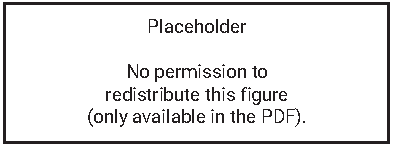
\includegraphics[width=1\textwidth]{gestalt-continuity}
\caption{\label{fig:continuity} Continuity makes the left-hand diagram easier to read (reproduced from \cite{Ware12} with permission).}
\end{marginfigure}

\begin{figure}
\centering
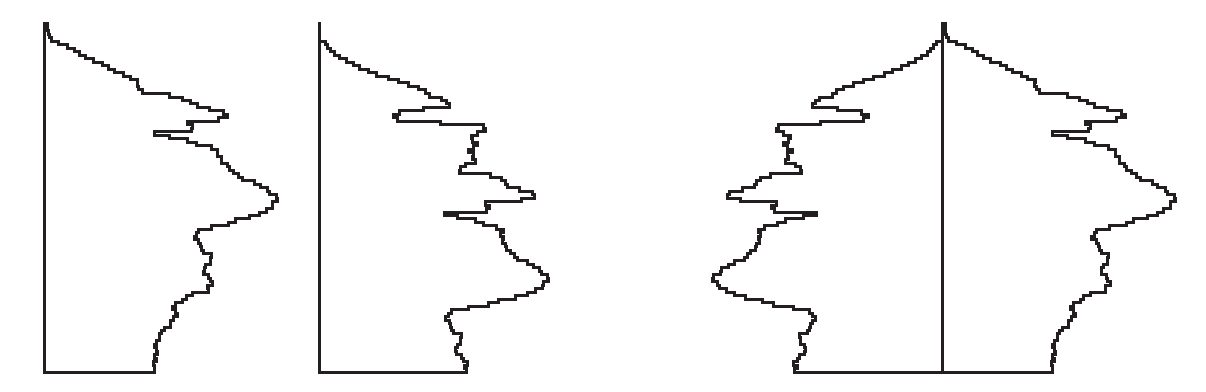
\includegraphics[width=1\textwidth]{gestalt-symmetry}
\sidecaption{\label{fig:symmetry} We can spot differences in these age distribution plots faster when data is plotted symmetrically (Data source: \url{https://destatis.de}, own illustration).}[-6\baselineskip]
\end{figure}

Another principle is \textbf{symmetry}. Symmetrical figures are visually pleasing, and we are good at detecting asymmetry. Symmetry is a form of high-level similarity. If you organize groups of elements in a diagram symmetrically, readers will assume that this means that they are similar. If you design diagrams asymmetrically, the asymmetric parts get emphasized. Our ability to check for symmetry can also be useful during visual data analysis (cf. Fig.~\ref{fig:symmetry}).

\begin{marginfigure}
\centering
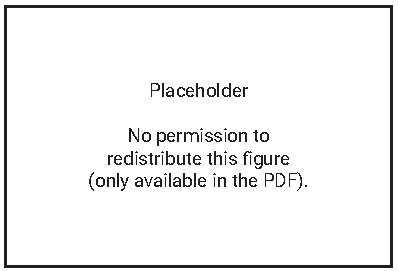
\includegraphics[width=1\textwidth]{gestalt-closure}
\caption{\label{fig:closure} Left: closure makes us perceive a full circle (reproduced from \cite{Ware12} with permission); right: the orange dot is perceived to sit inside of a rectangle.}
\end{marginfigure}

We are also on the lookout for \textbf{closure and common ground}. Closed contours are perceived as objects. Our search for closure is so strong that our brain interpolates missing parts of contours to form whole objects. As a result, we see a rectangle and a complete circle on the left-hand side of Fig.~\ref{fig:closure} instead of a circle with a missing segment. Moreover, contours create a notion of common ground with an ``inside'' and an ``outside''.

Common grounds are perceived for complete contours as well as for contours that we perceive due to closure. Thus, on the right-hand side of Fig.~\ref{fig:closure}, we perceive the orange dot to be inside an imaginary rectangle built by shapes. Ware recommends: ``Consider putting related information inside a closed contour. A line is adequate for regions having a simple shape. Color or texture can be used to define regions that have more complex shapes'' \cite{Ware12}.

The final Gestalt law to discuss is \textbf{figure and ground}. Figures are perceived as objects that are positioned in the foreground. The ground lies behind the figures. We perceive an object as a figure when it consists of a closed contour that forms a common ground and is considerably smaller compared to its surroundings.

\begin{marginfigure}
\centering
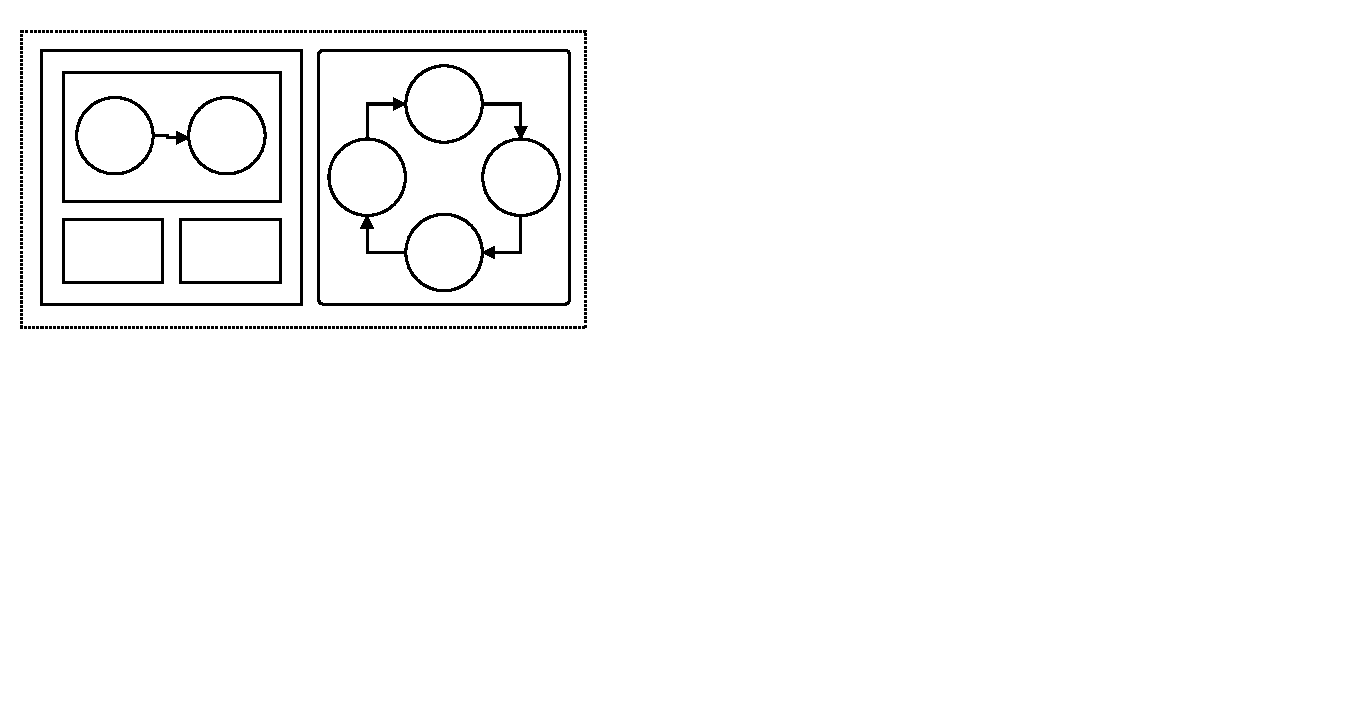
\includegraphics[width=1\textwidth]{gestalt-figureground}
\caption{\label{fig:figureground} Figure and ground are difficult to pick apart in this diagram; also note how PowerPoint fails to draw straight connectors (own illustration).}%[-1\baselineskip]
\end{marginfigure}

This principle is important when drawing diagrams that use contours to demarcate the boundaries of various systems. When multiple systems are nested, and the size differences are too small, it can become difficult to perceive the difference between figure and ground. Consider the diagram shown in Fig.~\ref{fig:figureground}). On the left-hand side of this diagram, too many rectangular shapes have been nested. Due to equal amounts of whitespace around every shape, multiple interpretations are possible. The right-hand side of the diagram is slightly better because the circles are considerably smaller than the surrounding rectangle. Moreover, together with the arrows the circles are perceived as a (symmetric) shape, which is easily perceived as a figure sitting on the rectangle in the background.


% Gestalt Theory and Instructional Design , Moore and Fitz 1993
% http://citeseerx.ist.psu.edu/viewdoc/download?doi=10.1.1.1026.6390&rep=rep1&type=pdf


\subsection{Color}
\label{sec:color}

You are probably used to defining colors in terms of red, green, and blue (RGB) or cyan, magenta, yellow, and black (CMYK). A third way, which is more useful, is the \textbf{HSB model}. It defines color in terms of hue, saturation, and brightness.\sidenote{Read the primer at \url{https://learnui.design/blog/the-hsb-color-system-practicioners-primer.html} for more details.} Consider the color picker shown in Fig.~\ref{fig:hsb} for an example.

\begin{figure}
\centering
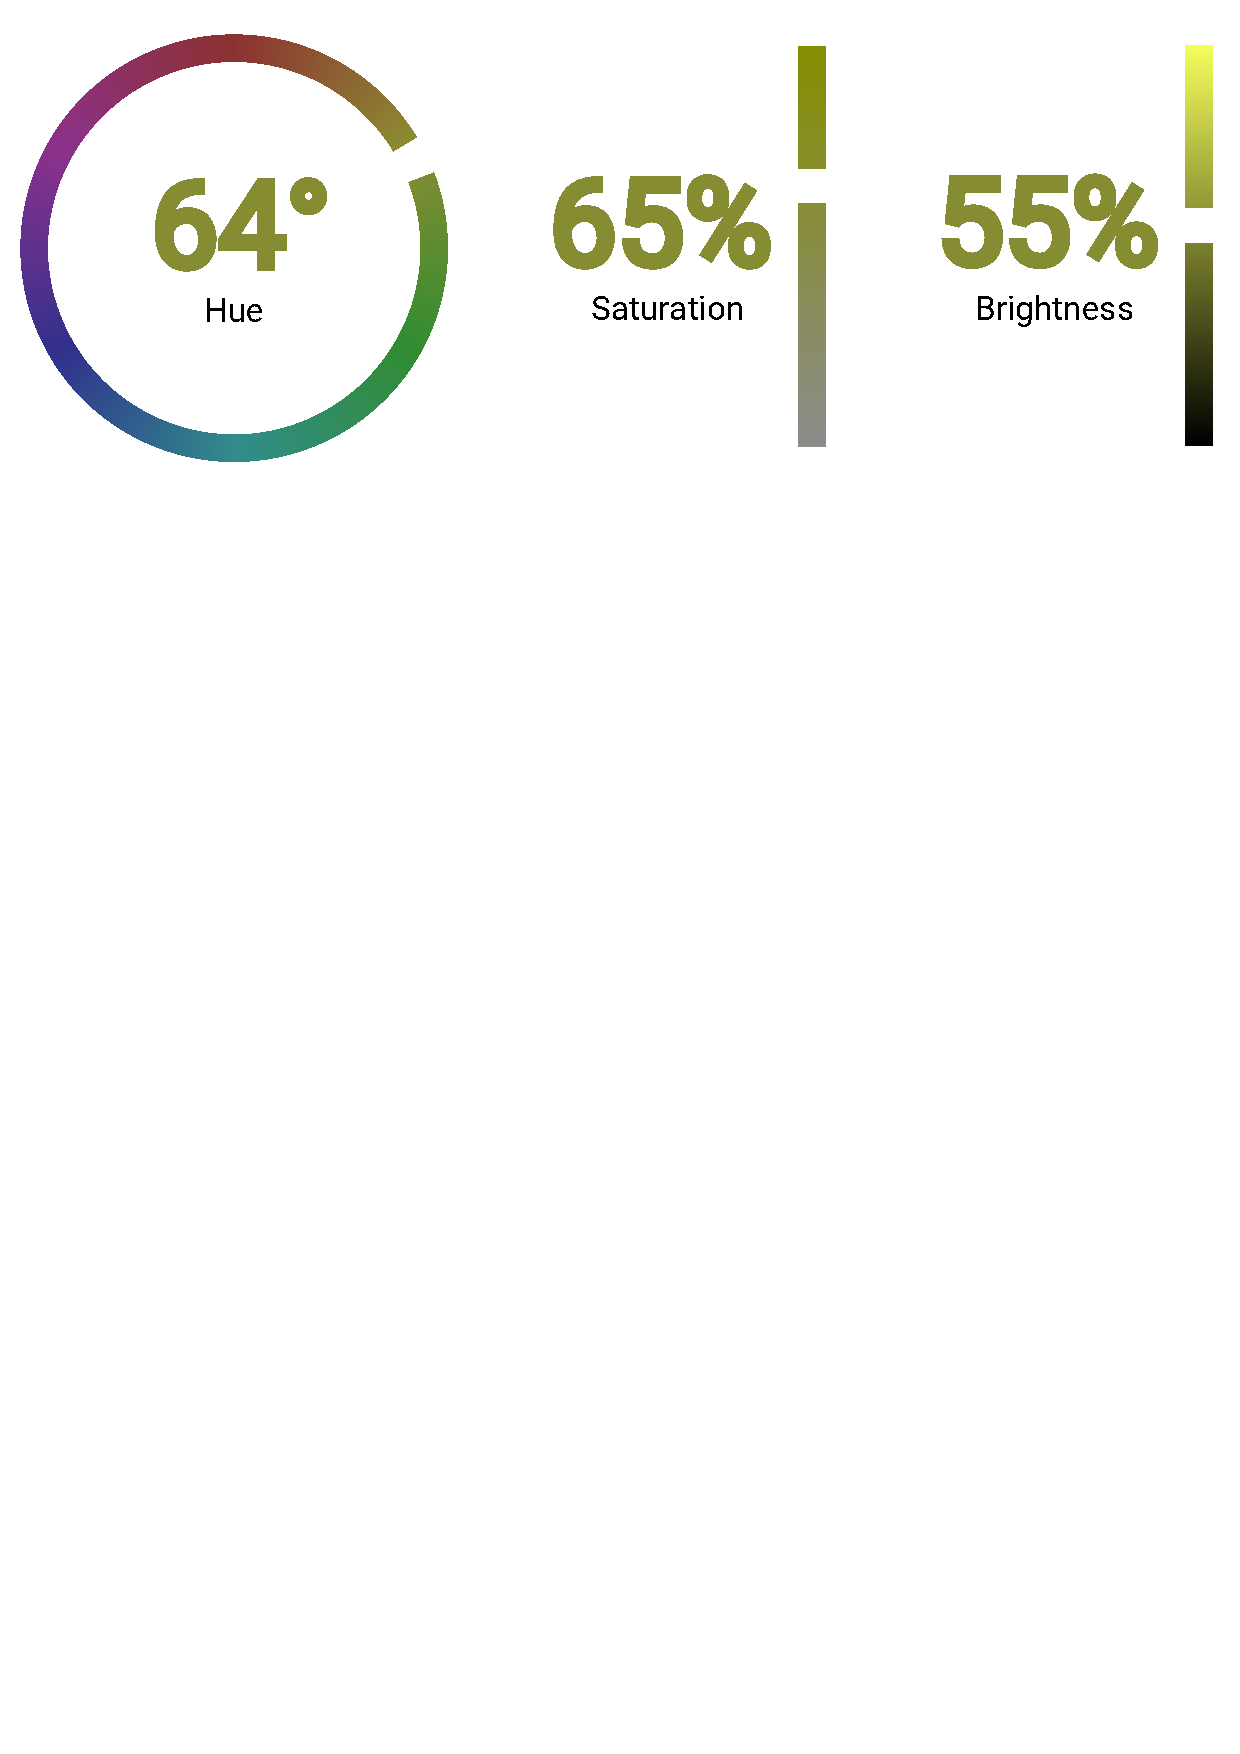
\includegraphics[width=0.85\textwidth]{color-hsb}
\sidecaption{\label{fig:hsb} A HSB color picker (\url{https://codepen.io/HunorMarton/full/eWvewo})}[-2\baselineskip]
\end{figure}

The first value, \textbf{hue}, defines the color according to its position (given in degrees ranging from 0 to 360) on the color wheel. For instance, the value of 60 corresponds to the hue yellow. \textbf{Saturation} (0 to 100) corresponds to the richness of the color, where 0 means that there is no trace of the hue, i.\,e., a gray color between white and black. The value 100 means that the hue is fully present, i.\,e., the color is as colorful as possible. The final value is \textbf{brightness} (0 to 100). A value of 0 corresponds to a solid black, a value of 100 corresponds to the brightest version of the hue at the given saturation.

\begin{marginfigure}
\centering
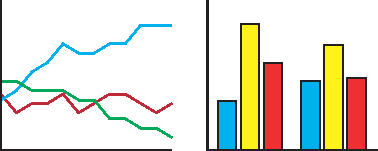
\includegraphics[width=1\textwidth]{color-plots}
\caption{\label{fig:coloredgraphs} Using colors to ease visual perception (reproduced from \cite{Carter12} with permission).}%[-1\baselineskip]
\end{marginfigure}

Different colors are often used to ease visual perception (cf. Fig.~\ref{fig:coloredgraphs}). For instance, it can be used for emphasis, to group subsets of elements, or to make it easier to distinguish different elements that have a similar shape.

Be aware of the monochrome representation of colors, which makes it impossible to distinguish a subset of colors. Red and green are particularly difficult to differentiate in monochrome print, especially if they have the same saturation and brightness (cf. Fig.~\ref{fig:monochrome}).

\begin{marginfigure}[-5\baselineskip]
\centering
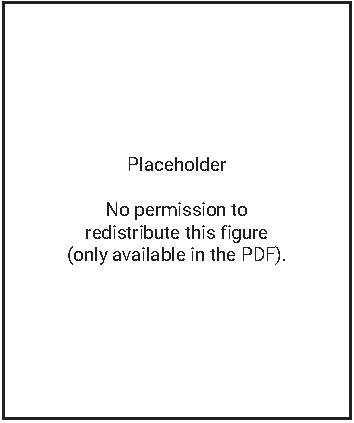
\includegraphics[width=0.8\textwidth]{color-mono}
\caption{\label{fig:monochrome} Colors in monochrome (reproduced from \cite{Carter12} with permission).}
\end{marginfigure}

The risk of confusion in monochrome prints is not the only reason why changing the hue is problematic. Different hues are difficult to make out when the area is small, as in the line plot in  Fig.~\ref{fig:coloredgraphs}. Moreover, different colors (hues) have different connotations (such as green means good, red means danger). Finally, different colors have a different visual weight that may create unwanted emphasis (blue is heavier than orange).

Therefore, it is often better to stick with one hue and use different levels of brightness or saturation to ease visual perception. Figure~\ref{fig:monographs} uses three shades of gray and is easier to read than the colorful version in Fig.~\ref{fig:coloredgraphs}.


\begin{marginfigure}
\centering
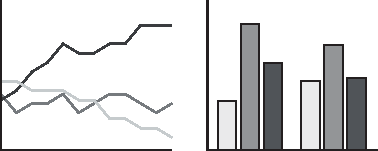
\includegraphics[width=1\textwidth]{color-plots-mono}
\caption{\label{fig:monographs} Shades of gray can be very effective (reproduced from \cite{Carter12} with permission).}%[-1\baselineskip]
\end{marginfigure}

When you use more than four different grayscale colors, however, the differences become too small to perceive with ease. Too many grayscale colors are especially problematic when color is used on its own, such as in line plots. It is less problematic in bar plots, because the bars can be sorted with decreasing brightness levels to create (good) redundancy. If brightness is used to encode values of data, darker colors should be used for higher values.

Similar principles apply for saturation: ``If using color saturation to encode numerical quantity, use greater saturation to represent greater numerical quantities. Avoid using a saturation sequence to encode more than three values'' \cite{Ware12}. Consider varying both brightness and saturation at the same time to create shades that are easier to distinguish from another.

\begin{marginfigure}
\centering
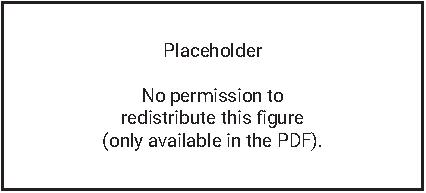
\includegraphics[width=1\textwidth]{color-saturation}
\caption{\label{fig:saturation} Use less saturation for large shapes, and more for thin lines (reproduced from \cite{Ware12} with permission).}%[-2\baselineskip]
\end{marginfigure}

The effects of different levels of saturation vary depending on the size of the colored area (cf. Fig.~\ref{fig:saturation}). If you consider varying saturation, stick to the following guidelines: ``Use more saturated colors when color coding small symbols, thin lines, or other small areas. Use less saturated colors for coding large areas'' \cite{Ware12}.


\section{Organizing Information}
\label{sec:organizinginfo}

In this section, we will review selected design concepts to organize information in a meaningful way. The book by Lidwell et al. contains more information on the ideas \cite{Lidwell10}.

\subsection{Advance Organizer}

An often-cited principle for giving a speech is summarized as follows: first, you announce what you are going to talk about; second, you talk about that; third, you review what you talked about. A design concept that implements this advice is an \emph{advance organizer}. Advance organizers are short chunks of information that are presented before new material. This way, readers will find it easier to learn new concepts.

Note that an advance organizer is not just a summary or an abstract. Its purpose is to relate new pieces of information to previously covered material and explain how this fits into the big picture. There are two kinds of advance organizers: expository and comparative.

\emph{Expository advance organizers}, as Lidwell et al. \cite{Lidwell10} explain, ``are useful when audiences have little or no knowledge similar to the information being taught.'' Expository advance organizers are effective when they provide a concise overview of the new material and how it fits together and into the big picture.

On the other hand, \emph{comparative advance organizers} ``are useful when audiences have existing knowledge similar to the information being presented. [They] compare and contrast features and operations between the familiar and the new'' \cite{Lidwell10}.

You can create advance organizers in the form of diagrams or as plain text. As a first step, you can add a \emph{signpost paragraph} at the beginning of chapters and sections.

\subsection{Hierarchy}

Complicated relationships are often explained using a hierarchical approach. 
There are three basic ways to represent hierarchy: trees, nests, and stairs (cf. Fig.~\ref{fig:hierarchy}).


\begin{marginfigure}
\centering
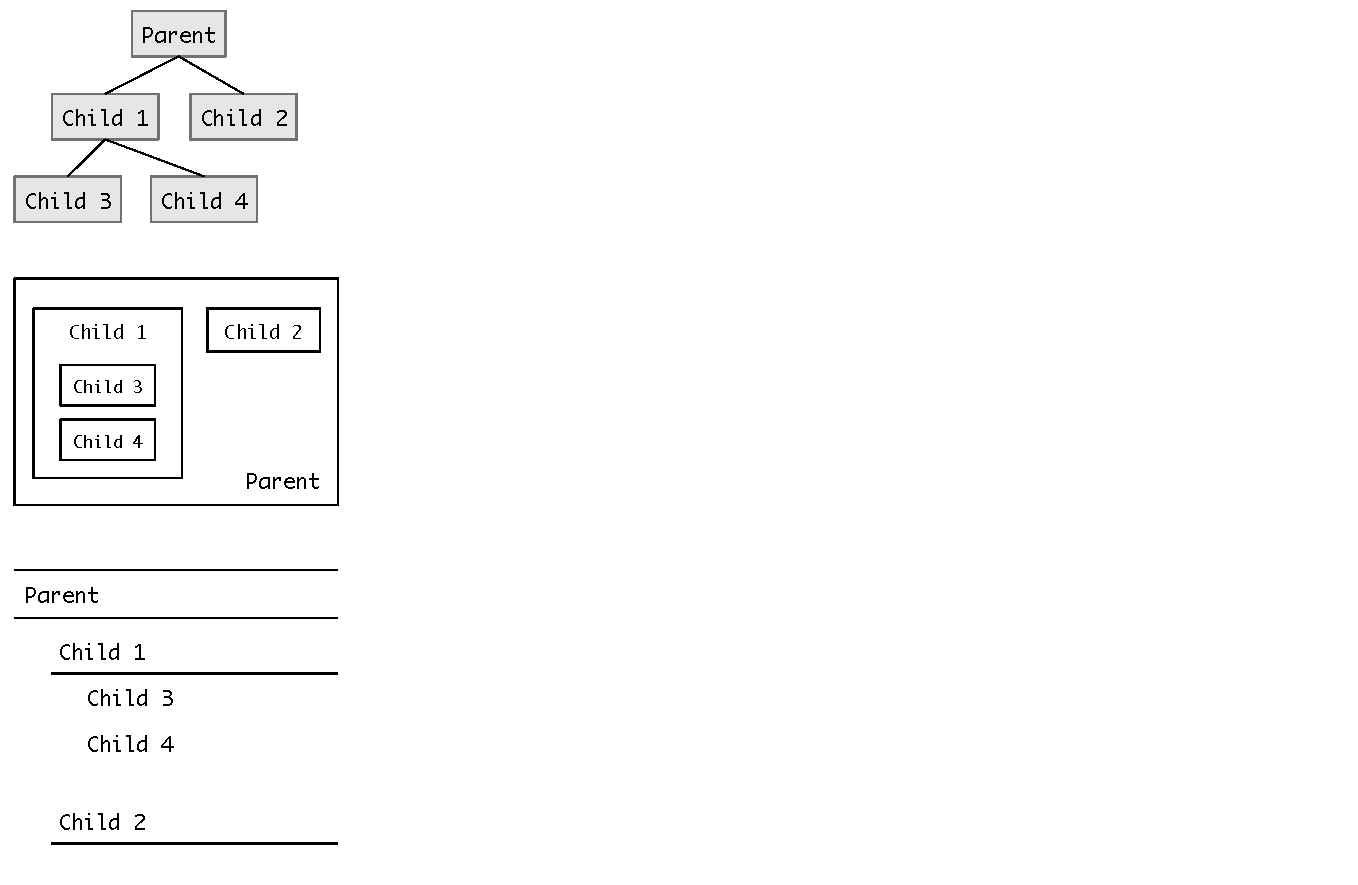
\includegraphics[width=1\textwidth]{info-orga-hierarchy}
\caption{\label{fig:hierarchy} You can visualize hierarchies with trees, nests, and stairs (own illustration).}%\cite{Lidwell10}.} 
\end{marginfigure}


\emph{Trees} are useful to visualize structures that consist of parent-child relationships such as A dominates B and C, B dominates of D and E, and so on. 
Usually, child elements are located below or to the right of their parents. As Lidwell et al. \cite{Lidwell10} observe, ``tree structures grow large quickly, and become tangled when multiple parents share common child elements. Tree structures are commonly used to represent overviews or high-level maps of system organization.''

\emph{Nest visualizations} are especially useful in visualizing parent elements that \emph{contain} child elements. Nest visualizations can be challenging to read when relationships are complicated.

Finally, \emph{stair structures} stack child elements below and to the right of parent elements. Stair visualizations are common in outlines. They can be used to capture arbitrarily complex hierarchies, especially when used interactively and individual nodes can be collapsed. Stair visualization also has a disadvantage: it may falsely imply a sequential relationship between the stacked child elements.

\subsection{Five Ways of Organization}
\label{sec:fivehatracks}

The so-called \emph{Five Hat Racks} design principle suggests five common ways to organize information: by category, time, location, alphabet, and continuum \cite{Lidwell10}.

\begin{enumerate}
\item \textbf{Organization by category} relies on similarity or relatedness of elements. Sometimes, categories can be organized hierarchically fashion.Note, Category is a nominal attribute, i.\,e., there is no natural order. If categories \emph{have} to be ordered, you can rely on alphabetical order or use an apparent order such as ``start with all the \emph{normal} categories, followed by the special ones.''

\item \textbf{Organization by time} is based on some chronological sequence. Ordering by time feels very natural. Note, however, that a chronological organization is not always useful. A literature review that merely presents one paper after another chronologically will not generate much insight.

\item \textbf{Organization by location} relies on geographical or spatial properties of the elements. Location can also be purely a logical concept, for instance, components that make up a system (which is also a hierarchy). It is common to describe systems by explaining one component (location) after another.

\item \textbf{Alphabetical organization} is another common technique. As Lidwell et al. \cite{Lidwell10} remark, ``organize information alphabetically, when information is referential, when efficient nonlinear access to specific items is required, or when no other organizing strategy is appropriate.''

\item \textbf{Organization by continuum} relies on a numeric property of the elements (e.\,g., ordering from highest to lowest or best to worst). Lidwell et al. \cite{Lidwell10} recommend to ``organize information by continuum when comparing things across a common measure.'' Organization by continuum can improve the readability of bar plots (cf. Fig.~\ref{fig:continuum})
\end{enumerate}


\begin{marginfigure}
\centering
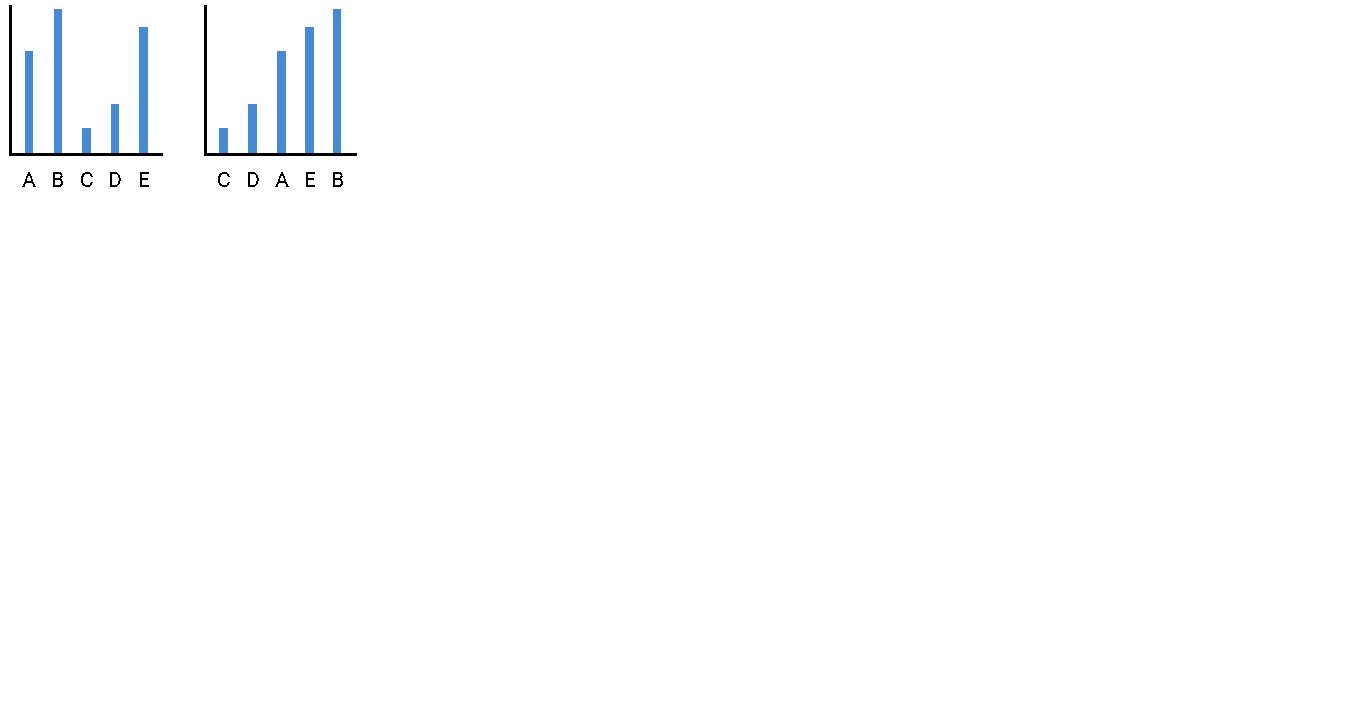
\includegraphics[width=1\textwidth]{info-orga-continuum}
\caption{\label{fig:continuum} Bar plots benefit from ordering the bars by length, an application of organization by continuum (own illustration).}%\cite{Lidwell10}.} 
\end{marginfigure}


\section{Diagrams}

You can use diagrams to describe concepts and their relationship, the structure of systems, interactions, and (experimental) procedures.

%\subsection{Common Problems}
% infohq
% examples

\subsection{Before You Start}

Your first task is to decide \emph{whether a visualization makes sense at all}. Sometimes it makes sense to choose a text-only representation such as pseudo-code instead of a diagram. Ware \cite{Ware12} shares the example of a flow chart, which is supposed to make it easier to understand the program flow (cf. Fig.~\ref{fig:flowchart}). He argues that pseudo code is superior. After all, the flow chart takes more effort to parse than the natural language used in the pseudo code (and, as Edward Tufte would argue, the flow chart contains more visual clutter than the pseudo code).

\begin{figure}[t]
\centering
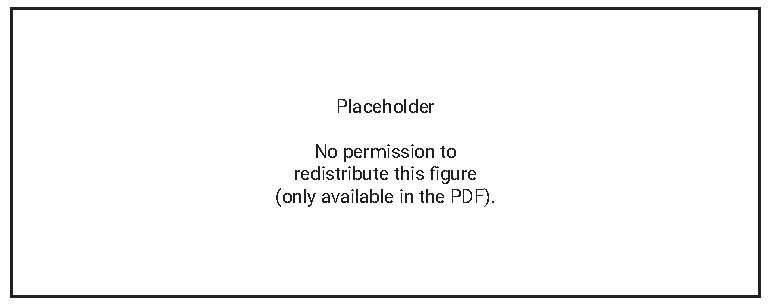
\includegraphics[width=1\textwidth]{diagram-flowchart}
\decoRuleFlex{1\textwidth}
\sidecaption{\label{fig:flowchart} In comparison to pseudo code a flow chart is a poor representation of program flow (reproduced from \cite{Ware12} with permission).}[-6\baselineskip]
\end{figure}

On the other hand, Ware argues, there are concepts that we can grasp much faster if we see a visual representation. Consider the following statements about a management hierarchy \cite{Ware12}:

\begin{itemize}
  \item Jane is Jim’s boss.
  \item Jim is Joe’s boss.
  \item Anne works for Jane.
  \item Mark works for Jim.
  \item Anne is Mary’s boss.
  \item Anne is Mike’s boss
\end{itemize}


\begin{marginfigure}
\centering
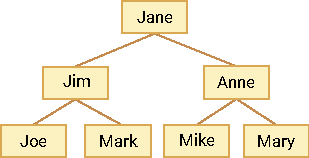
\includegraphics[width=1\textwidth]{diagram-tree}
\caption{\label{fig:tree} A tree helps us grasp static relationships (reproduced from \cite{Ware12} with permission).}%[-2\baselineskip]
\end{marginfigure}

It is challenging to keep track of all relationships in this presentation. You might even feel the urge to draw a tree. And, indeed, a graphical representation is much more accessible (cf. Fig.~\ref{fig:tree}). Ware concludes: ``Diagrams should be used to express structural relationships among program elements, whereas words should be used to express detailed procedural logic'' \cite{Ware12}.


Now, if you decide that you do want to create a diagram, you should ask yourself the following questions \cite{Carter12}:
\begin{itemize}
\item What is absolutely necessary to show?
\item What is not necessary to show?
\item What is most important and should be emphasized?
\item What is not important and should be secondary to the main message?
\item What are the relationships between individual elements?
\item Does the diagram require a precise depiction of time?
\item Does the diagram require a precise depiction of distance?
\item What symbols should be consistent throughout the diagram?
\end{itemize}

In the following sections, we will explain the most important aspects to create useful diagrams.

\subsection{Elements and Relationships}

According to the Gestalt laws, you should
``use small, closed shapes to represent data entities, and use the color, shape, and size of those shapes to represent attributes of those entities'' \cite{Ware12}. Figure~\ref{fig:entities} shows the effect of different properties of shapes.

\begin{figure}[t]
\centering
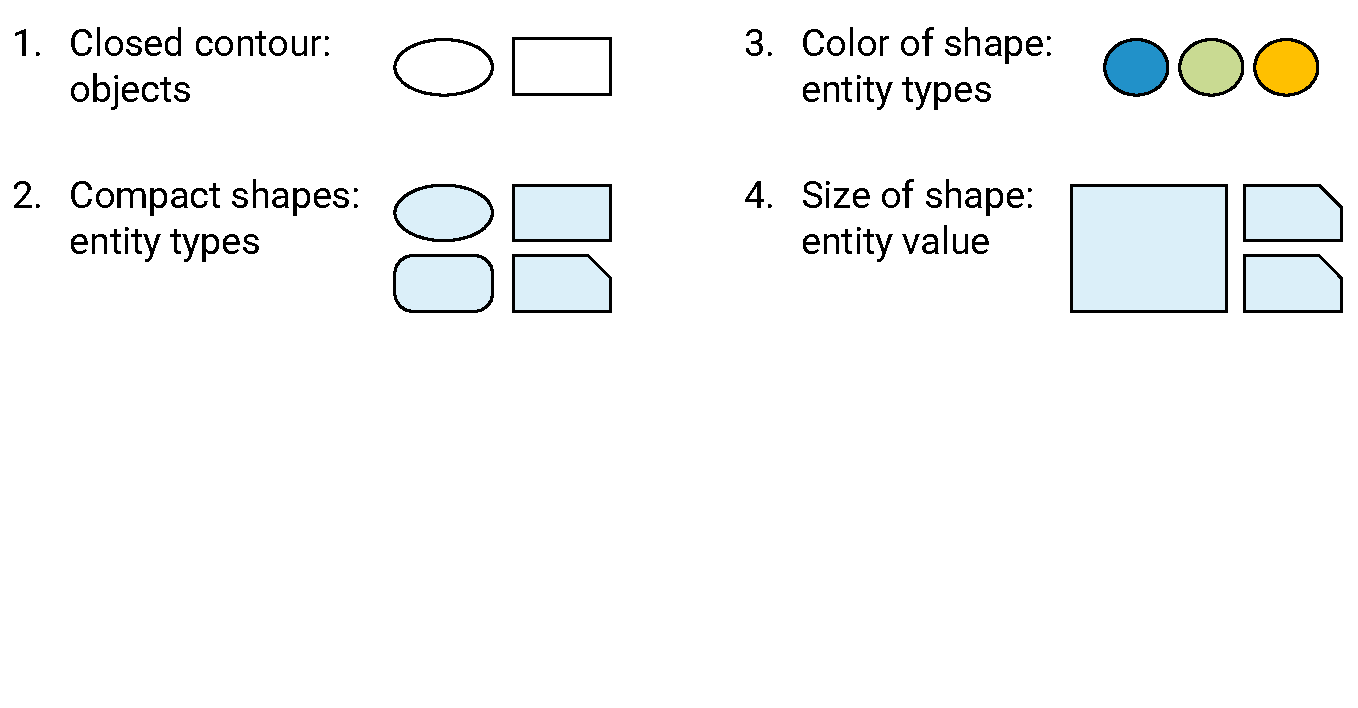
\includegraphics[width=1\textwidth]{diagram-entities}
\sidecaption{\label{fig:entities} Semantics of four properties of shapes (reproduced from \cite{Ware12} with permission).}[-5\baselineskip]
\end{figure}

Many diagrams are supposed to visualize relationships of elements. Ware recommends to use ``connecting lines, enclosure, grouping, and attachment to represent relationships between entities. The shape, color, and thickness of lines and enclosures can represent the types of relationships'' \cite{Ware12}. Figure~\ref{fig:relationships} visualizes ten alternatives and how we perceive them.

Of note are the tapered lines in Number 6 of Fig.~\ref{fig:relationships}. As explained by Ware, these are easier to recognize than arrows \cite{Ware12}, especially in busy diagrams. If you only use straight lines, you can use skinny triangles to create tapered lines. The broad end is located at the source of the line.

For more complex lines, you need a vector drawing tool like Inkscape, Adobe Illustrator, and Affinity Designer. Such tools also allow you to draw the wiggly line shown in Number 7 of Fig.~\ref{fig:relationships}. Most drawing tools enable you to create shapes with receptacles (cf. Number 9 of Fig.~\ref{fig:relationships}) by creating unions and differences of shapes.



\begin{figure}[t]
\centering
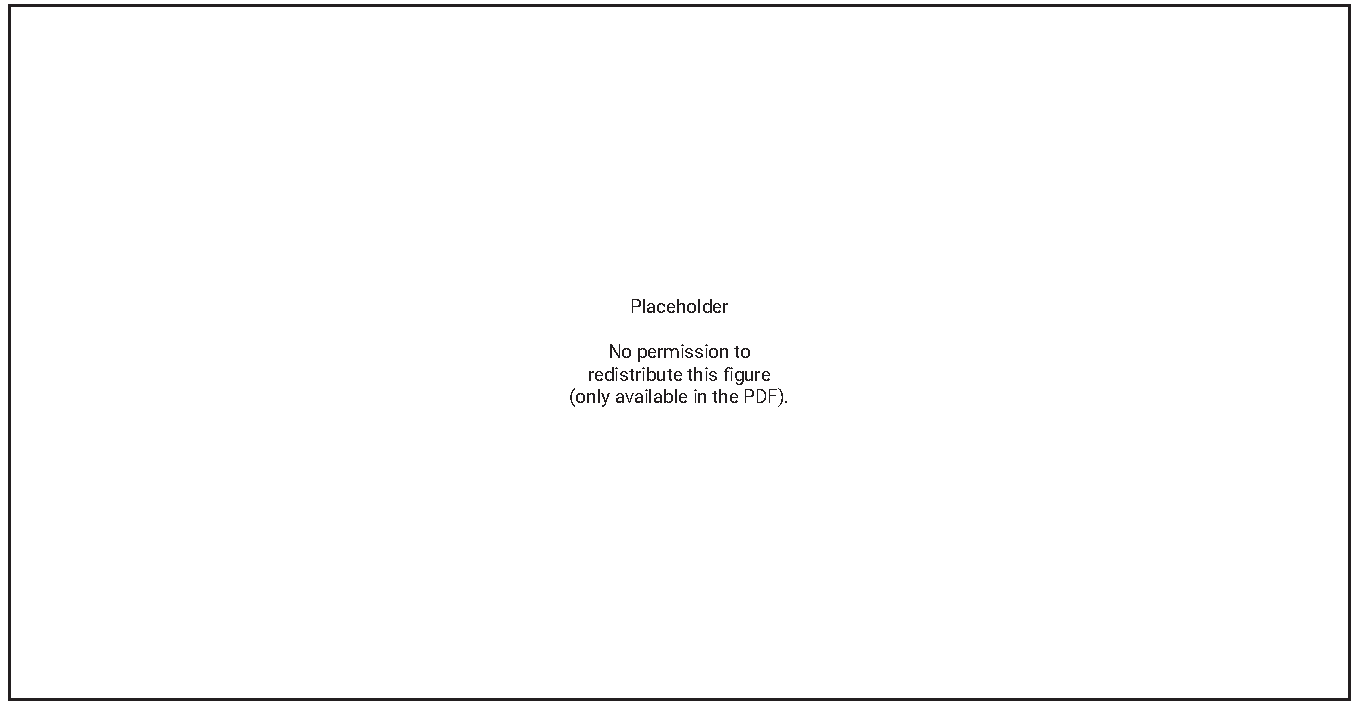
\includegraphics[width=1\textwidth]{diagram-relationships}
\sidecaption{\label{fig:relationships} Semantics of ten types of visual relationships (reproduced from \cite{Ware12} with permission).}[-5\baselineskip]
\end{figure}



\subsection{Emphasizing Elements}

Useful diagrams are self-explanatory and guide the reader's attention. Humans continuously search for patterns and deviations. Consistent use of shapes and colors indicates that the presented elements are similar (cf. Fig.~\ref{fig:emphasis}). Deviations from the norm indicate differences that need attention. Be aware of that, and do not create emphasis unintentionally.

\begin{figure}[t]
\centering
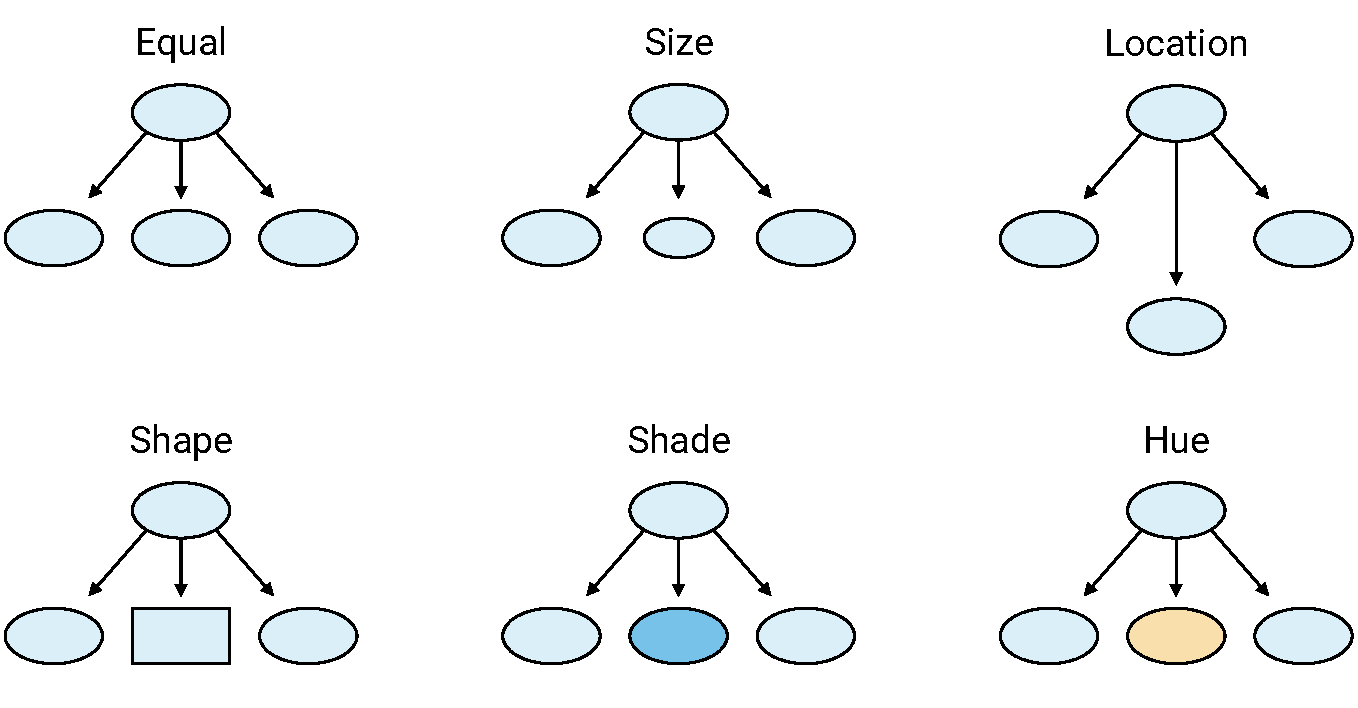
\includegraphics[width=1\textwidth]{diagram-emphasis}
\sidecaption{\label{fig:emphasis} Deviations from the norm create emphasis (reproduced from \cite{Carter12} with permission).}[-6\baselineskip]
\end{figure}

Do not choose the size of elements arbitrarily. Differences translate into dominance relationships. Larger elements usually appear to control the smaller ones (cf. Fig.~\ref{fig:dominance})

\begin{figure}[t]
\centering
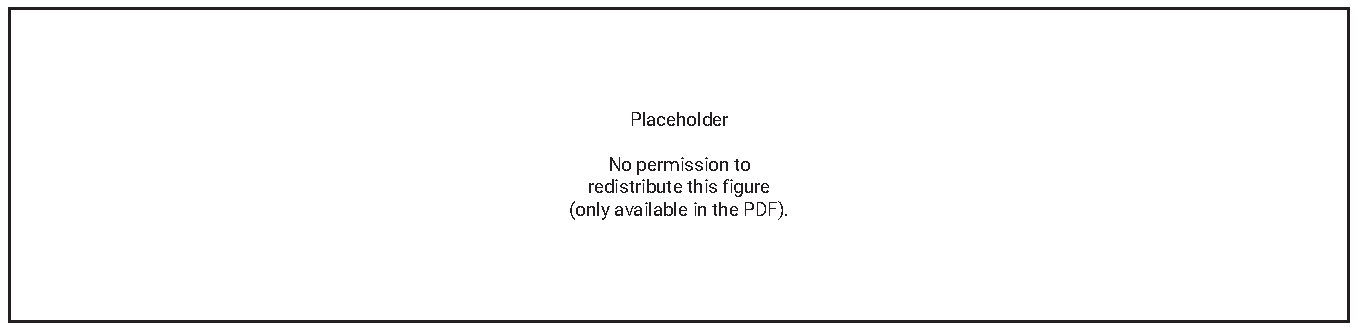
\includegraphics[width=1\textwidth]{diagram-dominance}
\sidecaption{\label{fig:dominance} Relative differences in size indicate dominance relationships (reproduced from \cite{Carter12} with permission).}[-6\baselineskip]
\end{figure}


\subsection{Layout}

In the absence of strong emphasis, readers process diagrams similar to text (cf. Fig.~\ref{fig:direction}). In western cultures, readers will start in the top left corner and proceed horizontally in a zig-zag pattern. The general flow of information should be consistent with this expectation.

\begin{marginfigure}
\centering
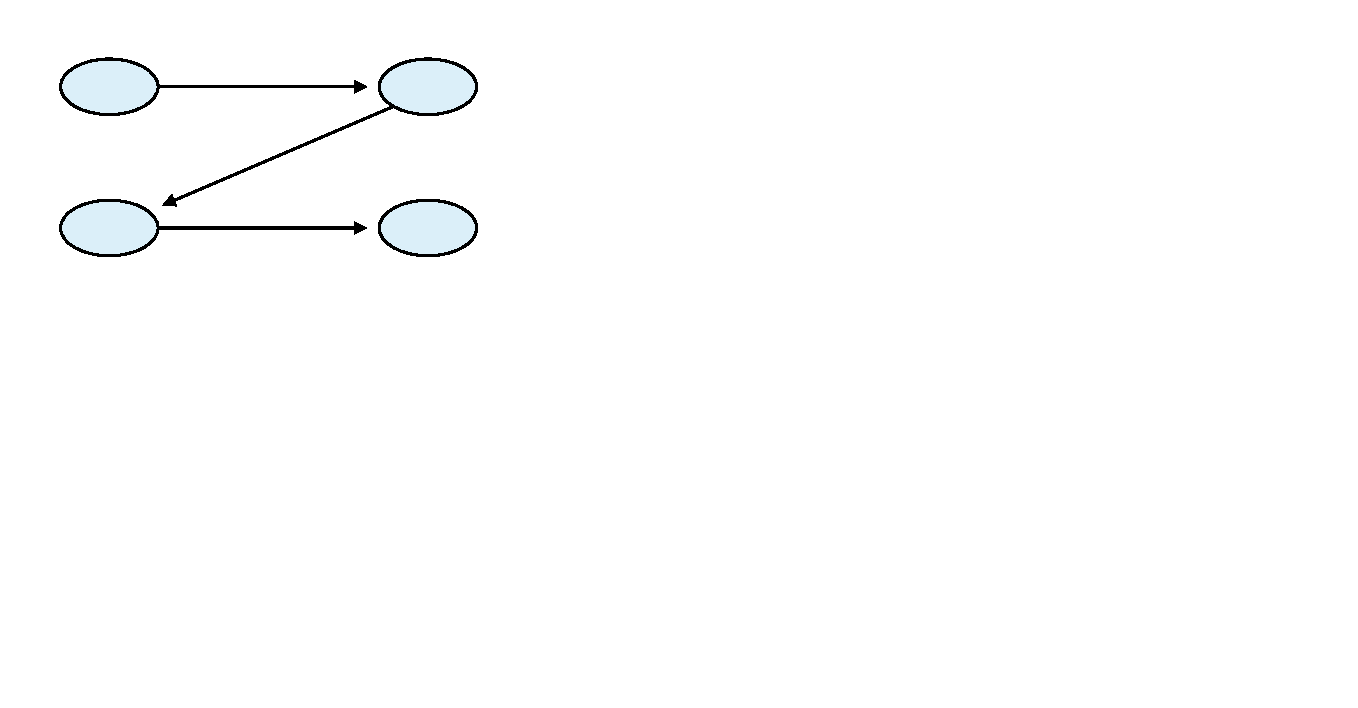
\includegraphics[width=1\textwidth]{diagram-direction}
\caption{\label{fig:direction} Respect the expected flow of information in western cultures (reproduced from \cite{Carter12} with permission).}%[-1\baselineskip]
\end{marginfigure}


Ensure that all elements of a diagram are correctly aligned. Alignment helps readers to grasp the overall structure. Proper alignment can also save you from creating additional outlines to depict (systems) boundaries – proximity and neat alignment can create strong cohesion by themselves (closure).

Make conscious decisions about distances and dimensions (proximity, repetition). You \emph{can} use a \emph{grid} to enforce consistent distances. Note, however, that snapping every element to the grid lines, may \emph{still} cause misalignment.\sidenote{Consider a shape that is five grid lines high. Then, a horizontal line that leaves the box cannot be aligned in the middle.} Make use of the horizontal and vertical alignment tools that space out elements equally. An advanced technique is to create a dummy box shape to measure and compare dimensions yourself.

\subsection{Labels}

Many diagrams consist of shapes and lines, annotated with text labels.

A common technique is to use bold print to express some property of an element. For instance, the labels of shapes corresponding to systems are printed in bold to differentiate them from the shapes that correspond to exchanged messages. In general, we recommend avoiding this practice. Reserve bold print to emphasize \emph{one particular element} in a diagram. Use another visual style to show differences, such as shading, colors, or shape form. Consider giving an element no surrounding shape at all, for instance, if the notion of its \emph{boundary} is not relevant or if the arrangement of sub-elements establishes a common ground due to the Gestalt law of \emph{closure}.

In any case, the labels should be as close as possible to the shapes (Gestalt law proximity) and precisely aligned. Whenever possible, consider moving the labels \emph{into} the shapes (Fig.~\ref{fig:labelsinside}). Inside labels rely on the Gestalt law of \emph{common ground}. They reduce visual clutter and make it easier to create a well-balanced diagram with no ragged edges (laws of symmetry and closure). 

\begin{figure}[t]
\centering
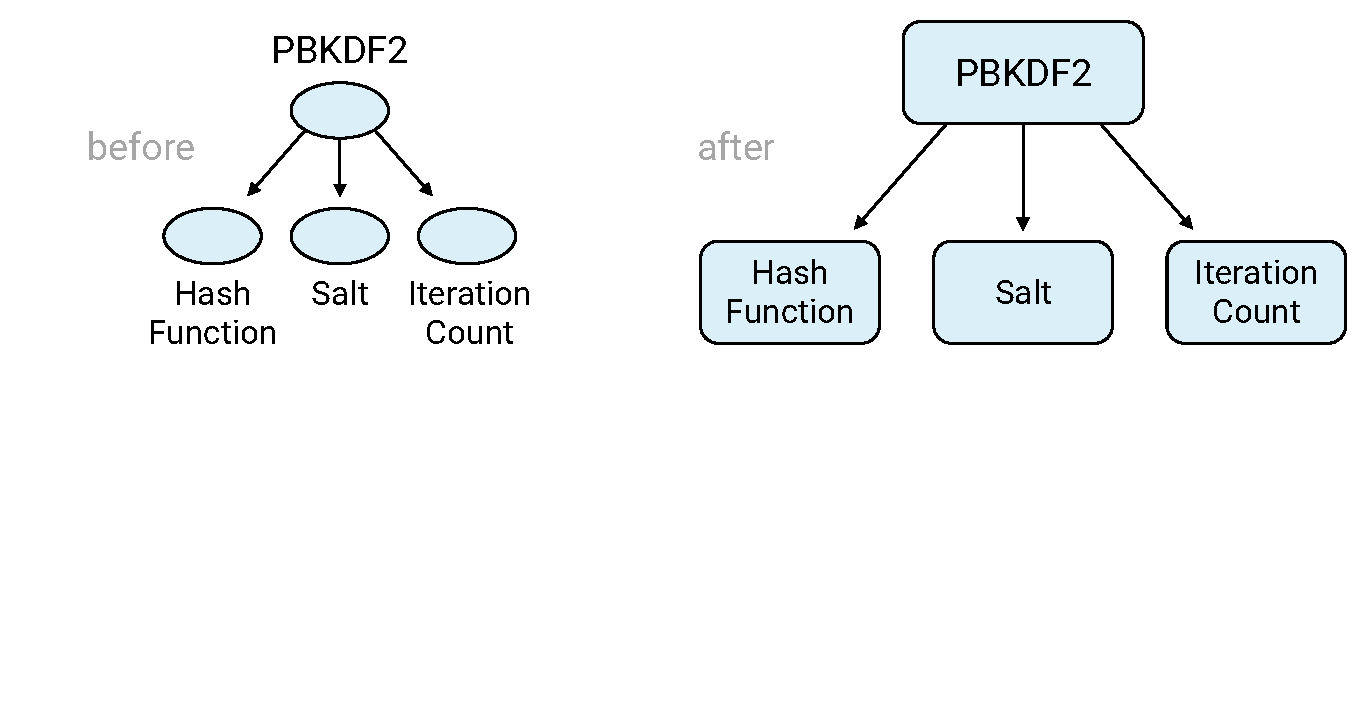
\includegraphics[width=1\textwidth]{diagram-labelsinside}
\sidecaption{\label{fig:labelsinside} Moving the labels inside objects reduces clutter. Note how the left-hand-side figure is centered in the left part of the figure to keep the figure balanced (reproduced from \cite{Carter12} with permission).}[-6\baselineskip]
\end{figure}

\begin{marginfigure}
\centering
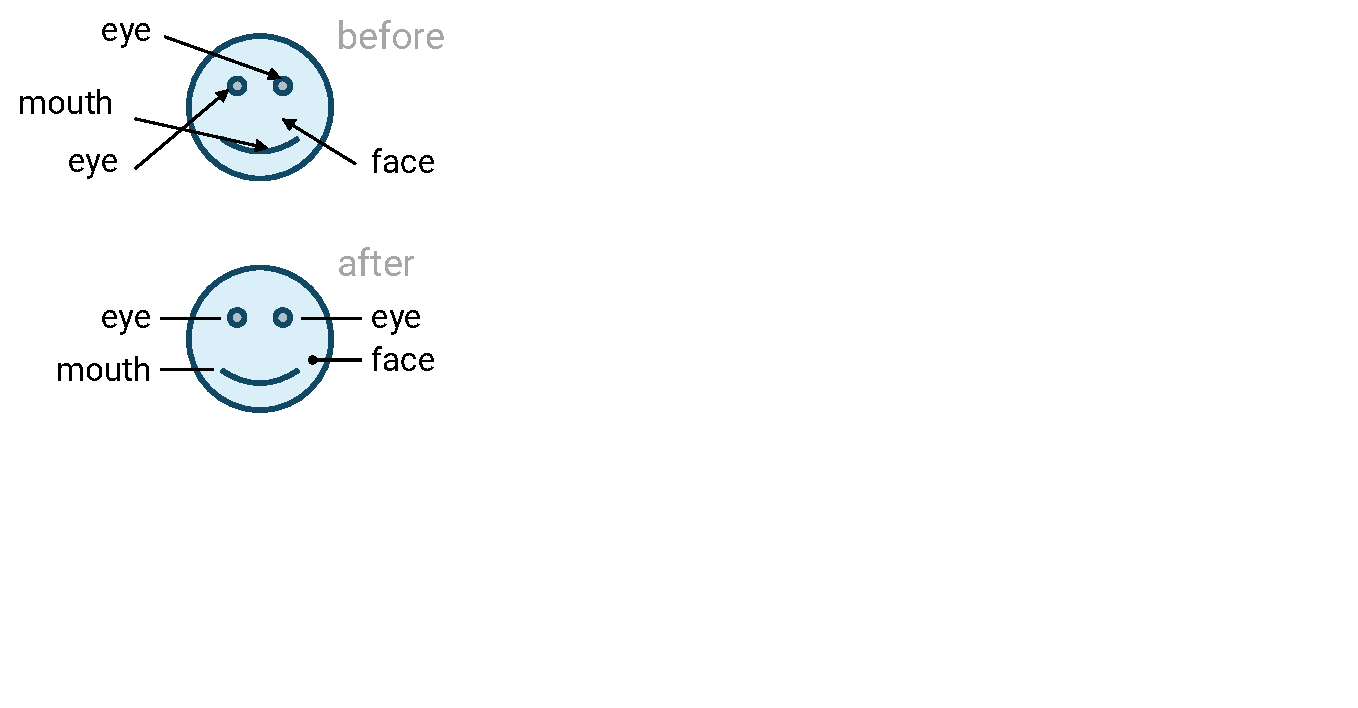
\includegraphics[width=1\textwidth]{diagram-labelsoutside}
\caption{\label{fig:labelsoutside} Outside labels should not distract the reader (own illustration, inspired by \cite{Carter12}).}%[-1\baselineskip]
\end{marginfigure}

Figure~\ref{fig:labelsoutside} illustrates critical principles when labels are \emph{outside} of a shape. First of all, keep the lines as short as possible (proximity). Consider removing the arrowheads from the lines that point into an object to avoid confusion with other arrows in the diagram. Also, avoid crossing lines. Align labels on the left-hand side of an object flush right and vice versa (symmetry). Aim for consistency by making the lines parallel. Keep adequate amounts of surrounding whitespace.

Diagrams that visualize structures can work fine with few labels. In contrast, diagrams that visualize procedures or more complex relationships need more textual explanation. Consider adding longer descriptions right next to the corresponding locations (proximity) as shown in Fig.~\ref{fig:explanations}.

\begin{figure}[t]
\centering
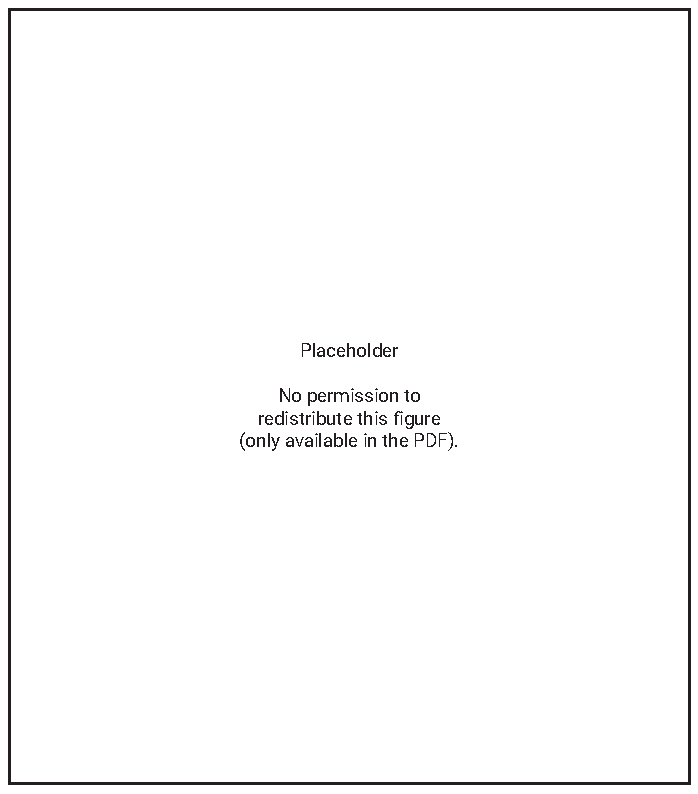
\includegraphics[width=1\textwidth]{diagram-explanations} 
\sidecaption{\label{fig:explanations} Complex diagrams benefit from integrated explanations. Source of figure as cited by \cite{Ware12}: R Chandler and J. Sweller (1991). Cognitive load theory and the format of instruction. \emph{Cognition and Instruction}, 8:4, 293–332, DOI: 10.1207/s1532690xci0804\_2, \url{www.tandfonline.com}. This figure is not subject to the Creative Commons License under which this guide is published (cf. Sect.~\ref{sec:license}); copyright is held by the publisher and/or the authors.}[-9\baselineskip]
\end{figure}


\subsection{Variations}

\begin{figure*}[t]
\centering
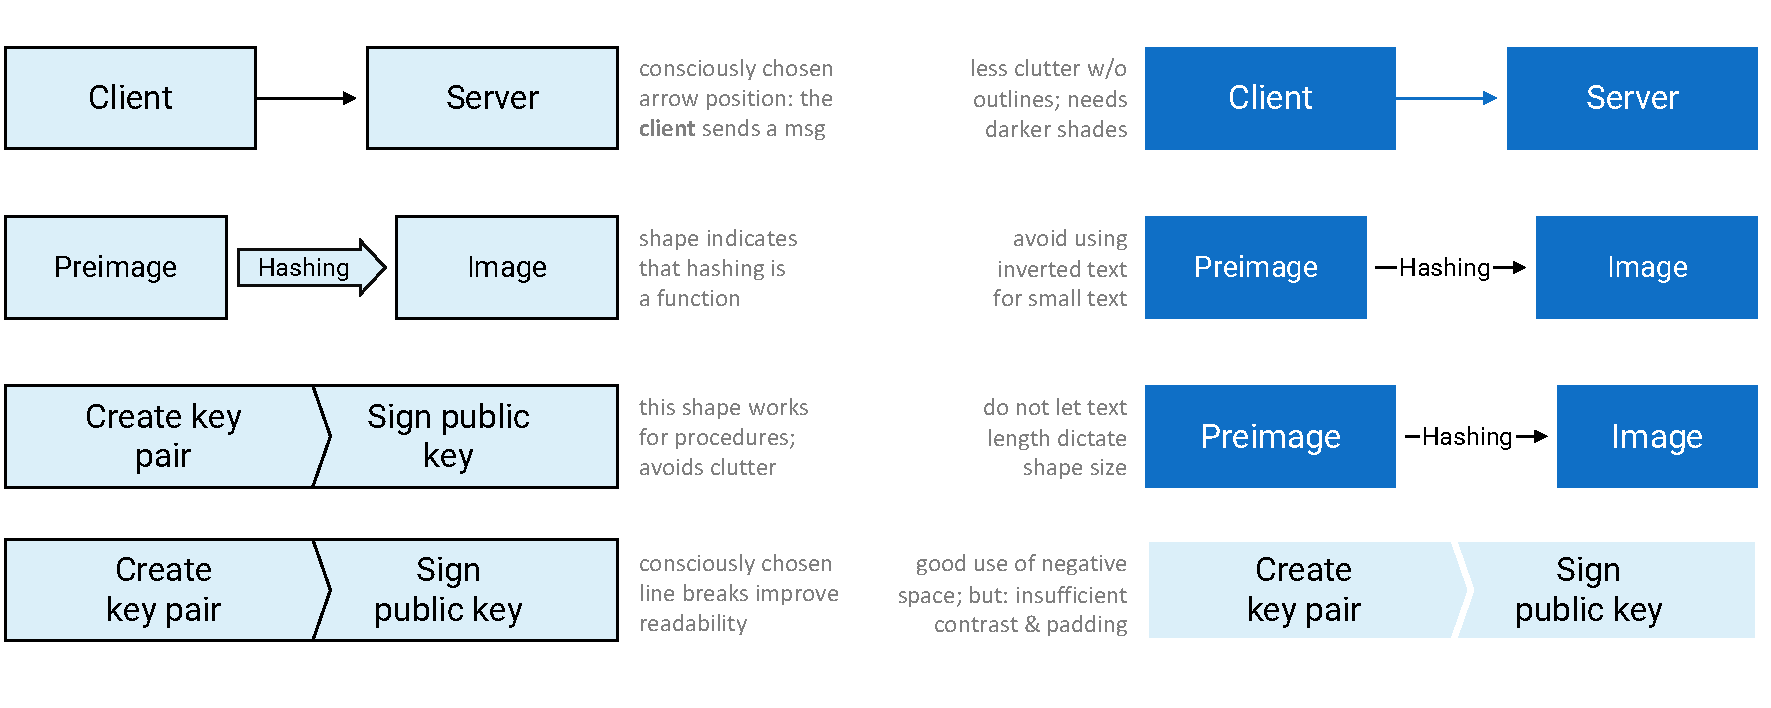
\includegraphics[width=1\widefigurewidth]{diagram-variations}
\sidecaption{\label{fig:diagvariations} Eight variations resulting from combining different outline, shade, and arrow styles.}[-1\baselineskip]
\end{figure*}

Common drawing tools provide a large number of shapes. What is missing, however, is guidance on how to combine them reasonably. Figure~\ref{fig:diagvariations} displays eight combinations.\sidenote{The advice in the following paragraphs has been compiled from \url{https://www.slideshare.net/otikik/how-to-make-awesome-diagrams-for-your-slides/19-Size_doesnt_mean_long_name}.}

The first variation in the left-hand column shows a style useful for depicting information exchange between systems, such as servers and clients. The second variation uses an arrow shape, which emphasizes the activity represented by the arrow. The third and fourth examples in the left-hand column depict two steps from a process without too much visual clutter. We prefer the latter one because the text wraps at sensible points.

The right-hand column shows variations without outlines. At first glance, this sounds like a good  idea: it avoids visual clutter (the outlines). Note, however, that shapes without outlines need more saturated and darker color to differentiate them from the background.  If the number of shapes in a diagram is large, this approach can make it more difficult to read the diagram because all shapes appear to be emphasized simultaneously.

If you use dark shapes, you should avoid having white text on dark background for small font sizes. As shown in the second variation on the right-hand side of Fig.~\ref{fig:diagvariations}, you will have to make changes to some shapes.

In any case, you should choose the sizes of shapes consciously. Represent objects with identical properties with shapes of the same size. If the labels do not fit into the shapes, you can either reduce the font size, put the labels next to the box, or increase the size of all shapes (by rearranging the diagram).

Finally, consider the option of using negative space, as shown in the bottom-right corner of Fig.~\ref{fig:diagvariations}. Again, this can be a useful means to avoid visual clutter. However, if you increase the width of the surrounding white stroke (as was done for the example figure), the (vertical) padding in the shape will become too narrow. Moreover, you cannot easily align such shapes with other shapes with thinner strokes.


\section{Graphs}

In this section, we review common design principles for graphs (also called charts or plots). Besides our guidelines, we will present the examples shown by Carter \cite{Carter12}.

The first step in data visualization is to \textbf{pick a reasonable chart type}. Most visualization needs that arise in a thesis can be addressed with line charts, bar charts, and histograms, and scatter plots. There are many more chart types such as Chord Diagrams, Sankey Diagrams, and the Nightingale Rose Chart.\sidenote{For comprehensive overviews and guidance see \url{https://datavizcatalogue.com}, \url{https://depictdatastudio.com/charts/}, \url{https://www.data-to-viz.com/img/poster/poster_big.png} and \url{https://www.labnol.org/images/2008/data-chart-type.png}.}
These and other advanced chart types \emph{can} be useful in particular situations. In general, however, we recommend sticking to more basic chart types. In particular, \textbf{avoid pie charts} unless you know what you are doing.

General advice for any graph is to have \textbf{legible axis labels} and, if more than one data series is visualized, a legend for the data series. Moreover, remember to use colors effectively (cf. Sect.~\ref{sec:color}).

The following sections provide more information on two essential chart types, line charts and bar charts. The recommendations are very concrete. You may find that you cannot follow all of them using your plotting tool of choice. If this limitation bothers you, consider editing the plotting tool's output with a vector drawing program such as Inkscape or Adobe Illustrator.

\subsection{Line Charts}

Line charts show how one variable (the one on the y-axis) changes when another one varies within a given range. Line charts are particularly useful to visualize time series.

Often, there are many lines to be plotted. Resist the temptation to add more than three lines into one line chart if the lines overlap. Instead, create multiple charts that have one of the lines in common. This line serves as a baseline, easing comparison.

Figure~\ref{fig:linecharts} summarizes Carter's advice on line charts.

\begin{figure*}[t]
\centering
%\vspace{3\baselineskip}

\includegraphics[width=1\widefigurewidth]{graphs-linecharts}
\sidecaption{\label{fig:linecharts} Advice for line charts (reproduced from \cite{Carter12} with permission). %Remark on the layout: As seen in this case, putting a wide figure below another one does not look very pleasing.
}[-1\baselineskip]
\end{figure*}

\subsection{Bar Charts}

The top row of Fig.~\ref{fig:barcharts} summarizes Carter's advice on bar charts.
Bar charts are useful to compare the value of a single variable under different circumstances. The value of the variable corresponds to the length of a bar. In principle, a single bar chart can also show the values of \emph{different} variables. Note, however, that such a chart is more challenging to read, especially when the variables need differently scaled Y-axes (one to the left and one to the right of the chart).

The bars can be drawn horizontally and vertically.\sidenote{See \url{https://depictdatastudio.com/when-to-use-horizontal-bar-charts-vs-vertical-column-charts/} for more guidance.} It is common to use vertical bars for time series (time on the x-axis). You can also use vertical bars if the values on the x-axis are on an ordinal scale (i.\,e., they are arranged in their natural order). Vertical bars do not work well with long labels. Rotating labels makes them challenging to read. On the other hand, horizontal bar charts work well with longer labels (align the labels flush right next to the bars).

The advice in this section assumes vertical bars. In vertical bar charts, the Y-axis corresponds to the value of the variable, and the X-axis is typically used for a categorial variable, which represents the different circumstances.

An advanced version of a classical bar chart is a stacked bar chart, an excellent alternative to visualize proportions of a whole. In contrast, to pie charts, which can be deceiving, stacked bar charts are more accurate and can be easily compared.

\begin{figure*}[t]
\centering
\vspace{4\baselineskip}
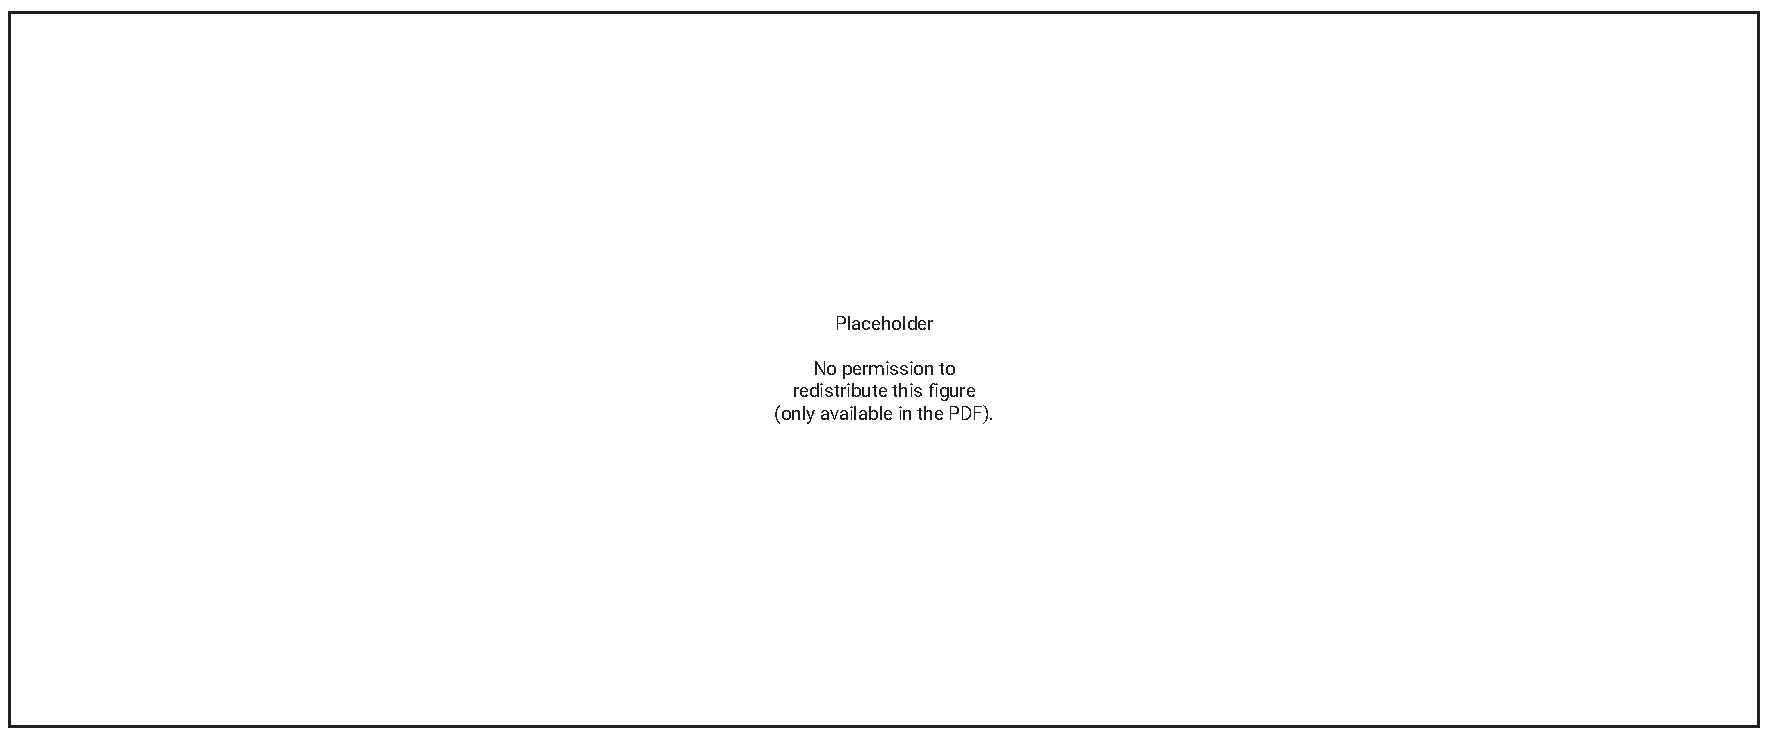
\includegraphics[width=1\widefigurewidth]{graphs-barcharts}

\bigskip


\includegraphics[width=1\widefigurewidth]{graphs-histograms}
\sidecaption{\label{fig:barcharts} Advice for bar charts and histograms (reproduced from \cite{Carter12} with permission).}
\end{figure*}

\paragraph{Histograms} A special kind of bar charts is a histogram. Carter gives a concise explanation of the purpose of a histogram: ``A histogram shows the distribution of data and the relative frequency with which the data occur. It essentially offers the audience an estimate of the probability distribution of a dataset'' \cite{Carter12}. The bottom row of Fig.~\ref{fig:barcharts} summarizes Carter's advice on histograms.

%\begin{figure*}[t]
%\centering
%\vspace{4\baselineskip}
%
\includegraphics[width=1\widefigurewidth]{graphs-histograms}
%\sidecaption{\label{fig:histograms} Advice for histograms \cite{Carter12}.}
%\end{figure*}






\section{Tables}
\label{sec:tableguide}

Tables are useful to display multiple properties for several entities. This section summarizes Carter's guidelines for designing effective tables \cite{Carter12}. Moreover, you will see how to apply the principles of organizing information (cf. Sect.~\ref{sec:organizinginfo}).

Often, the properties of entities have different scales and units. Readers usually expect that rows correspond to entities, and columns correspond to properties. This organization makes it easier to compare entities in terms of individual properties by focusing on the values in particular columns. It is easy to spot exceptional cases if they are printed vertically and the eye can move downwards. The example in Table~\ref{tab:colrows} shows this effect with two tables that contain the same data.

\begin{table*}[tb]
  \caption{\label{tab:colrows} The table to the left is easier to read than the table to the right (reproduced from \cite{Carter12} with permission).}
  \centering
  \footnotesize % use smaller fontsize in the table
  {\renewcommand{\arraystretch}{1.1} % increase vertical space between rows
  \begin{tabularx}{0.45\linewidth}{@{}Xccr@{}} % @{} omits outer horizontal margins, the "X" column uses up all remaining available space 
    \toprule
    Lake & Area ($\mathrm{km}^2$) & Length (km) & Depth (m)\\
    \midrule
    Malawi & 30,044 & 579 & 706 \\
    Tanganyika & 32,893 & 676 & 1470 \\
    Victoria & 59,485 & 322 & 84\\
    \bottomrule
  \end{tabularx}
  \hspace{\fill}
  \begin{tabularx}{0.45\linewidth}{@{}Xccr@{}} % @{} omits outer horizontal margins, the "X" column uses up all remaining available space 
    \toprule
    Lake & Malawi & Tanganyika & Victoria\\
    \midrule
    Area ($\mathrm{km}^2$) & 30,044 & 32,893 & 59,485 \\
    Length (km) & 579 & 676 & 322 \\
    Depth (m) & 706 & 1470 & 84\\
    \bottomrule
  \end{tabularx}
  }
\end{table*}

Follow the Gestalt principle of Hierarchy when you display information that can be grouped. Often, there is more than one way how to group data. Make a conscious decision about how you organize the table. Different forms of organization emphasize different aspects. For instance, the table to the left in Table~\ref{tab:groups} emphasizes the comparison between men and women. In contrast, the table to the right highlights the differences between the years.

\begin{table*}[tb]
\caption{Number of men and women selected by NASA to be astronauts by year of selection (reproduced from \cite{Carter12} with permission).}
\label{tab:groups}
\centering
\footnotesize % use smaller fontsize in the table
{\renewcommand{\arraystretch}{1.1} % increase vertical space between rows
  \begin{tabularx}{0.53\linewidth}{@{}Xcccccc@{}} % @{} omits outer horizontal margins, the "X" column uses up all remaining available space 
  \toprule
  & \multicolumn{3}{c}{\tabhead{Men}} & \multicolumn{3}{c}{\tabhead{Women}} \\
  \cmidrule(lr){2-4} \cmidrule(l){5-7}
  & \tabhead{1980} & \tabhead{1990} & \tabhead{2000} & \tabhead{1980} & \tabhead{1990} & \tabhead{2000}\\
  \midrule
  Mission specialist & 9 & 12 & 7 & 2 & 4 & 3\\
  Pilot &              8 &  6 & 7 & 0 & 1 & 0\\
  \midrule
  Total &             17 & 18 & 14 & 2 & 5 & 3\\
  \bottomrule
  \end{tabularx}
\hspace{\fill}
  \begin{tabularx}{0.42\linewidth}{@{}Xcccccc@{}} % @{} omits outer horizontal margins, the "X" column uses up all remaining available space 
  \toprule
  & \multicolumn{2}{c}{\tabhead{1980}} & \multicolumn{2}{c}{\tabhead{1990}} & \multicolumn{2}{c}{\tabhead{2000}}\\
  \cmidrule(lr){2-3} \cmidrule(lr){4-5} \cmidrule(l){6-7}
  & \tabhead{M} & \tabhead{F} & \tabhead{M} & \tabhead{F} & \tabhead{M} & \tabhead{F}\\
  \midrule
  Mission specialist & 9 & 2 & 12 & 4 & 7 & 3\\
  Pilot &              8 & 0 &  6 & 1 & 7 & 0\\
  \midrule
  Total &             17 & 2 & 18 & 5 & 14 & 3\\
  \bottomrule
  \end{tabularx}
}
\end{table*}

Make a conscious decision on how to order the columns. Revisit the five hat racks design principle in Sect.~\ref{sec:fivehatracks}. If there is no logical ordering, e.\,g.,  from very generic properties to more specific ones, order the columns alphabetically. Usually, derived pieces of information, results, and insights are to the right of labels and descriptive pieces of information.

Choosing an adequate order also applies to rows. Instead of sorting the rows alphabetically based on their label in the first column, consider sorting them based on a particular column's value. The resulting order can improve legibility a lot (principle of \emph{continuity}). Note that sorting the table by a specific column puts some emphasis on that particular column. This principle is visualized in Table~\ref{tab:roworder}.

\begin{table*}[tb]
  \caption{\label{tab:roworder} Listing planets in order from the sun, in alphabetical order, and in descending order of diameter (reproduced from \cite{Carter12} with permission).}
  \centering
  \footnotesize % use smaller fontsize in the table
  {\renewcommand{\arraystretch}{1.1} % increase vertical space between rows
  \begin{tabularx}{0.3\linewidth}{@{}Xrr@{}} % @{} omits outer horizontal margins, the "X" column uses up all remaining available space 
    \toprule
    Planet & Diameter & Mass \\
    \midrule
    Mercury & 0.38 & 0.06 \\
    Venus & 0.95 & 0.82 \\
    Earth & 1.00 & 1.00 \\
    Mars & 0.53 & 0.11 \\
    Jupiter & 11.21 & 317.80 \\
    Saturn & 9.45 & 95.20 \\
    Uranus & 4.01 & 14.60 \\
    Neptune & 3.88 & 17.20 \\
    \bottomrule
  \end{tabularx}
  \hspace{\fill}
  \begin{tabularx}{0.3\linewidth}{@{}Xrr@{}} % @{} omits outer horizontal margins, the "X" column uses up all remaining available space 
    \toprule
    Planet & Diameter & Mass \\
    \midrule
    Earth & 1.00 & 1.00 \\
    Jupiter & 11.21 & 317.80 \\
    Mars & 0.53 & 0.11 \\
    Mercury & 0.38 & 0.06 \\
    Neptune & 3.88 & 17.20 \\
    Saturn & 9.45 & 95.20 \\
    Uranus & 4.01 & 14.60 \\
    Venus & 0.95 & 0.82 \\
    \bottomrule
  \end{tabularx}
  \hspace{\fill}
  \begin{tabularx}{0.3\linewidth}{@{}Xrr@{}} % @{} omits outer horizontal margins, the "X" column uses up all remaining available space 
    \toprule
    Planet & Diameter & Mass \\
    \midrule
    Jupiter & 11.21 & 317.80 \\
    Saturn & 9.45 & 95.20 \\
    Uranus & 4.01 & 14.60 \\
    Neptune & 3.88 & 17.20 \\
    Earth & 1.00 & 1.00 \\
    Venus & 0.95 & 0.82 \\
    Mars & 0.53 & 0.11 \\
    Mercury & 0.38 & 0.06 \\
    \bottomrule
  \end{tabularx}
  }
\end{table*}
% Appendix C
 
\chapter{About the Template}
\label{appendixc}
\label{appendix-more-details-on-template}

This appendix provides additional information about less-often needed features of the template. Moreover, it contains a brief overview of the template's history. 

\section{Further Template Features}\label{ThesisFeatures}

This section explains customization options and technical details. For a thesis at the PSI Chair, you should stick with the defaults.

\subsection{Printing Format}

This thesis template is designed for double-sided printing (i.\,e., content on the front and back of pages) as most theses are printed and bound this way.\sidenote{At the PSI Chair, we highly encourage you to use double-sided printing.}
Switching to one-sided printing is as simple as uncommenting the \option{oneside} option of the \code{documentclass} command at the top of the \file{main.tex} file. You may then wish to adjust the margins to suit specifications from your institution.

The headers for the pages contain the page number on the outer side (so it is easy to flick through to the page you want) and the chapter name on the inner side.

The text is set to 11 point by default with single line spacing; again, you can tune the text size and spacing using the options at the top of \file{main.tex}. The spacing can be influenced by replacing the \option{singlespacing} with \option{onehalfspacing} or \option{doublespacing}.

\subsection{Using US Letter Paper}

The paper size used in the template is A4, which is the standard size in Europe. If you are using this thesis template elsewhere, for instance, in the United States, then you may have to change the A4 paper size to the US Letter size.

Due to the differences in the paper size, the resulting margins may be different to what you like or require. You may need to adapt the page geometry settings in \file{setup.tex} in this case.

\subsection{References}

The template uses \code{biblatex} to format the bibliography and references such as this one \cite{murdoch_steven_j._chip_2010}. The template uses a citation style that creates in-text citations with the author(s) initials and the year of the publication. Multiple references are separated by semicolons (e.\,g., \cite{solat_security_2017, bond_chip_2014}). To see how you use references, have a look at the source files of this guide. If you choose a suitable BibTeX reference manager, you can copy and paste or drag and drop references into the document.

The bibliography is typeset with references listed in alphabetical order by the first author's last name. To see how LaTeX typesets the bibliography, have a look at the very end of this document (or just click on the reference links in in-text citations).

\paragraph{BibTeX Backend}

As the ``old'' \code{bibtex} backend does not correctly handle Unicode character encoding (i.\,e., ``international'' characters), we use the more modern \code{biber} BibTeX engine in this template.

Here, we cite a lot of references so that the list of references gets populated \cite{murdoch_steven_j._chip_2010,anderson_ross_emv:_2014,kou_weidong_secure_2003,solat_security_2017,bond_chip_2014,ortiz_s._is_2006,haselsteiner_security_2006,galloway_visa_2019,zhou_nshield_2014,lalehTaxonomyFraudsFraud2009,ferradiWhenOrganizedCrime2016,Yang10,Kopsell06,VilaGM03,Herrmann12-ipv6prefix,Herrmann14-diss,HBF:2013,Herrmann11-NordSec,AcarEEJND14,Herrmann09,WangG13,Raymond00,Hintz02,Herrmann14-encdns,Goodson12-privacy,WendolskyHF07,chaum81,BertholdFK00,Dingledine04,rfc5246,LoesingMD10,FuchsHF13}.



\section{Contributors and History}

This guide has been written by Dominik Herrmann. The LaTeX template has been created by Dominik Herrmann with support by Fabian Lamprecht. Dominik and Fabian are affiliated with the Privacy and Security in Information Systems Group at University of Bamberg (\url{https://www.uni-bamberg.de/psi/}).


The PSI Template has its own \emph{document class}, \file{PSIThesis.cls}. It has been derived from \file{MastersDoctoralThesis.cls} (\url{https://www.latextemplates.com/template/masters-doctoral-thesis}).

The MastersDoctoralThesis LaTeX thesis template is based initially on a LaTeX style file created by Steve R.\ Gunn from the University of Southampton (UK), department of Electronics and Computer Science. You can find his original thesis style file at his site at
\url{http://www.ecs.soton.ac.uk/~srg/softwaretools/document/templates/} (link not available as of 2019).

Steve's \file{ecsthesis.cls} was then taken by Sunil Patel, who modified it by creating a skeleton framework and folder structure for a thesis. The resulting template is available on Sunil's site at
\url{http://www.sunilpatel.co.uk/thesis-template}.

Sunil's template was made available through \url{http://www.LaTeXTemplates.com} where it was modified many times based on user requests and questions. Version 2.0 and onwards of this template represents a significant modification to Sunil's template and is, in fact, hardly recognizable. The work to make version 2.0 possible was carried out by \href{mailto:vel@latextemplates.com}{Vel} and Johannes Böttcher.


\section{License}
\label{sec:license}

This guide and the template are made available under the Creative Commons license 
CC BY-SA 4.0 (\url{http://creativecommons.org/licenses/by-sa/4.0/}) with two exceptions:

\begin{enumerate}
\item Some excerpts, figures, and tables in Chapter~2 and Appendix~B have been taken from the
literature. The respective elements are explicitly marked with a citation and a note
regarding the permission to re-use. They are not
covered by the CC license. Permission to re-use and distribute
these figures, tables, and excerpts must be obtained from the
respective copyright holders.

\item Parts of \Cref{Chapter1} and \Cref{appendix-more-details-on-template} contain content from the
MastersDoctoralThesis template mentioned above, which is licensed under 
CC BY-SA 3.0 (\url{http://creativecommons.org/licenses/by-nc-sa/3.0/}). 
The original content has been written by
Sunil Patel (\href{http://www.sunilpatel.co.uk}{www.sunilpatel.co.uk}) and
Vel (\href{http://www.LaTeXTemplates.com}{LaTeXTemplates.com}).
\end{enumerate}

As the guide contains copyrighted material, you should not host your own copy of this guide online.

The files \texttt{PSIThesis.cls}, \texttt{setup.tex}, and \texttt{titlepage.tex} are made available under
the LPPL v1.3c (\url{http://www.latex-project.org/lppl}).




%----------------------------------------------------------------------------------------
%	BIBLIOGRAPHY
%----------------------------------------------------------------------------------------

% Bibliography has no wide margins:
\newgeometry{
	inner=2cm, % Inner margin
	outer=2cm, % Outer margin
	marginparwidth=0cm,
	marginparsep=0mm,
	bindingoffset=.5cm, % Binding offset
	top=1.5cm, % Top margin
	bottom=2.5cm, % Bottom margin,
	includehead,
	includefoot
	% showframe, % Uncomment to show how the type block is set on the page
}

\addchap{References}

% enables two-column layout for bibliography
\setlength\columnsep{2em}
\begin{multicols}{2}
	\begin{refcontext}[sorting=nyt] % sort bibliography by last name, year, title
		\renewcommand*{\bibfont}{\small\RaggedRight}
		\linespread{1.0}\selectfont % increase linespread if desired (not recommended)
		\printbibliography[heading=none]
	\end{refcontext}
\end{multicols}

%----------------------------------------------------------------------------------------

%----------------------------------------------------------------------------------------
%	DECLARATION PAGE
%----------------------------------------------------------------------------------------

\begin{declaration}
\addchaptertocentry{\authorshipname} % Add the declaration to the table of contents

% TODO Change the declaration according as needed. *

%\selectlanguage{ngerman}
Ich erkläre hiermit gemä\ss\ \S~17 Abs.\,2 APO, dass ich die vorstehende {\thesistype}arbeit selbständig\\ verfasst und keine anderen als die angegebenen Quellen und Hilfsmittel benutzt habe.

\bigskip
\bigskip

\begin{tabular}{@{}l@{}}
  Bamberg, den \rule[-0.8em]{10em}{0.5pt}\\[2ex]
  ~
\end{tabular}
\hspace{\fill}%
\begin{tabular}{@{}c@{}}
  \rule[-0.8em]{20em}{0.5pt}\\[2ex]
  \authorname
\end{tabular}\hspace{\fill}




\end{declaration}

\end{document}
